
\documentclass{compositio}

\usepackage[english]{babel}
%\usepackage{geometry}
\usepackage{amsmath,amssymb,amsthm}

%fonts I chose for the arXiv version
%\usepackage{palatino}
%\usepackage{newpxmath}

%\usepackage{yfonts}
\usepackage[T1]{fontenc}
\usepackage[utf8x]{inputenc}
%\usepackage{enumerate}
\usepackage{enumitem}
\usepackage{verbatim}
\usepackage{graphicx}
\usepackage{faktor}
\usepackage{xcolor}
\usepackage{xfrac}
\usepackage{tikz,tikz-cd}
\usepackage{hyperref}
\usepackage[normalem]{ulem}
\usepackage{setspace}

\usepackage{calrsfs}
\DeclareMathAlphabet{\pazocal}{OMS}{zplm}{m}{n}


\newcommand{\tropC}{\scalebox{0.8}[1.3]{$\sqsubset$}}
%\newcommand{\ttropC}{\widetilde{\tropC}}
\newcommand{\tropT}{\scalebox{0.9}[1.2]{$\top$}}
%\newcommand{\tropD}{\scalebox{0.9}[1.3]{$\triangle$}}

\newcommand{\M}[4]{\overline{\pazocal M}_{#1,#2}(#3,#4)}
\newcommand{\PP}{\mathbb P}
\renewcommand{\k}{\mathbf k}
\newcommand{\m}{\mathfrak m}
\newcommand{\tR}{\widetilde{R}}
\newcommand{\tm}{\widetilde{\mathfrak m}}
\newcommand{\OO}{\mathcal O}
\renewcommand{\to}{\rightarrow}
\newcommand{\pr}{\rm{pr}}
\newcommand{\Aaff}{\mathbb A}
\newcommand{\N}{\mathbb N}
\newcommand{\oM}{\overline{\pazocal M}}
\newcommand{\tM}{\widetilde{\pazocal M}}
\newcommand{\R}{\operatorname{R}}
\newcommand{\Gm}{\mathbb{G}_{\rm{m}}}
\newcommand{\Ga}{\mathbb{G}_{\rm{a}}}
\newcommand{\vir}[1]{[#1]^{\rm{vir}}}
\newcommand{\virloc}[1]{[#1]^{\rm{vir}}_{\rm{loc}}}
\newcommand{\dvr}{\Delta}

\newcommand{\bq}{\begin{equation}}
\newcommand{\eq}{\end{equation}}
\newcommand{\ba}{\begin{aligned}}
\newcommand{\ea}{\end{aligned}}
\newcommand{\be}{\begin{enumerate}}
\newcommand{\ee}{\end{enumerate}}
\newcommand{\bsm}{\left(\begin{smallmatrix}}
\newcommand{\esm}{\end{smallmatrix}\right)}                   
\newcommand{\bpm}{\begin{pmatrix}}
\newcommand{\epm}{\end{pmatrix}}
\newcommand{\barr}{\begin{displaymath}\begin{array}{cccc}}
\newcommand{\earr}{\end{array}\end{displaymath}}
\newcommand{\barrl}{\begin{displaymath}\begin{array}{lcl}}
\newcommand{\earrl}{\end{array}\end{displaymath}}
\newcommand{\barl}{\begin{displaymath}\begin{array}{l}}
\newcommand{\earl}{\end{array}\end{displaymath}}
\newcommand{\bxym}{ \begin{displaymath}\xymatrix }
\newcommand{\exym}{\end{displaymath}}
\newcommand{\bcd}{\begin{center}\begin{tikzcd}}
\newcommand{\ecd}{\end{tikzcd}\end{center}}

\newcommand{\tr}{{\rm tr}}
\newcommand{\Isom}{\text{Isom}}
\newcommand{\Spec}{\underline{\operatorname{Spec}}}
\newcommand{\Proj}{\operatorname{Proj}}
\newcommand{\Pic}{\operatorname{Pic}}
\newcommand{\Hom}{\operatorname{Hom}}
\newcommand{\dist}{\operatorname{dist}}
\newcommand{\hhom}{\mathcal{H}\!om}
\newcommand{\Aut}{\operatorname{Aut}}
\newcommand{\Exc}{\operatorname{Exc}}
\newcommand{\lev}{\operatorname{lev}}
\newcommand{\id}{{\rm id}}

\theoremstyle{plain}
\newtheorem{thm}{Theorem}[section]
\newtheorem{lem}[thm]{Lemma}
\newtheorem{prop}[thm]{Proposition}
\newtheorem{cor}[thm]{Corollary}
\newtheorem*{theorem*}{Theorem}
\newtheorem*{fact}{Fact}

\theoremstyle{definition}
\newtheorem{definition}[thm]{Definition}

\theoremstyle{remark}
\newtheorem{rem}[thm]{Remark}
\newtheorem*{caveat}{Caveat}
\newtheorem{claim}{Claim}

\hyphenation{Ca-roc-ci}


\usepackage{tikz,tikz-cd,tikz-3dplot}
\usepackage{pgfplots}
\usetikzlibrary{arrows,shadows,positioning, calc, decorations.markings, 
hobby,quotes,angles,decorations.pathreplacing,intersections,shapes}
\usepgflibrary{shapes.geometric}
\usetikzlibrary{fillbetween,backgrounds}

\tikzset{
  arrow/.pic={\path[tips,every arrow/.try,->,>=#1] (0,0) -- +(0,4pt);},
  pics/arrow/.default={triangle 90}
}

\tikzset{->-/.style={decoration={
  markings,
  mark=at position .6 with {\arrow{latex}}},postaction={decorate}}
  }

\tikzset{
  c/.style={every coordinate/.try}
}

\newcommand{\midarrow}{\tikz \draw[-triangle 90] (0,0) -- +(.03,0);}





\begin{document}

\title[Modular compactifications of $\pazocal{M}_{2,n}$]{Modular compactifications of $\pazocal{M}_{2,n}$ \\ with Gorenstein curves}
%
\author{Luca Battistella}
\email{lbattistella@mathi.uni-heidelberg.de}
\address{Ruprecht-Karls-Universität Heidelberg\\Im Neuenheimer Feld 205\\69120 Heidelberg\\Germany}
%
%\dedication{A dedication can be included here.}
\classification{14H10 (primary), 14H20 (secondary).}
\keywords{moduli of curves, Gorenstein singularities, genus two, crimping spaces}
\thanks{This project grew out of discussions with Francesca Carocci, whom I thank heartily. I am grateful to Daniele Agostini, Fabio Bernasconi, Sebastian Bozlee, Maria Beatrice Pozzetti, Dhruv Ranganathan, Luca Tasin, and Jonathan Wise for helpful conversations. I thank the anonymous referee, whose quick response and precise sugestions greatly helped improving the exposition of this material. I thank the Max Planck Institute for Mathematics in Bonn for providing financial support and a stimulating research environment. During the revision of this paper, I was supported by the Deutsche Forschungsgemeinschaft (DFG, German Research Foundation) under Germany’s Excellence Strategy EXC-2181/1 - 390900948 (the Heidelberg STRUCTURES Cluster of Excellence).}

\begin{abstract}
\setstretch{1.1}{
We study the geometry of Gorenstein curve singularities of genus two, and of their stable limits. These singularities come in two families, corresponding to either Weierstrass or conjugate points on a semistable tail. For every $1\leq m <n$, a stability condition - using one of the markings as a reference point, and thus not $\mathfrak S_n$-symmetric - defines proper Deligne-Mumford stacks $\oM_{2,n}^{(m)}$ with a dense open substack representing smooth curves.}
\end{abstract}

\maketitle


\section{Introduction}
We construct alternative compactifications of the moduli stack of smooth $n$-pointed curves of genus two. The boundary of the Deligne-Mumford compactification, consisting of stable nodal curves, is gradually replaced by ever more singular curves, complying with more restrictive combinatorial requirements on the dual graph. For $1\leq m <n$, we introduce a notion of $m$-stability, that allows Gorenstein singularities of genus one and two while at the same time demanding that higher genus subcurves contain a minimum number of special points. Our main result concerning the stack of $m$-stable curves is the following:
\begin{theorem*}
 $\oM^{(m)}_{2,n}$ is a \emph{proper} irreducible Deligne-Mumford stack over $\operatorname{Spec}(\mathbb Z[\frac{1}{30}])$.
\end{theorem*}
This paper fits into the framework of alternative compactifications and birational geometry of the moduli space of curves, extending work of D.I. Smyth in genus one, but we expect it to find applications to enumerative geometry as well.

We classify Gorenstein singularities of genus two with any number of branches, and their (semi)stable models, highlighting the relation with Brill-Noether theory. The key insight in defining the new stability conditions is that we can avoid non-Gorenstein singularities by modifying the curve at the conjugate point of the special branch; we use one of the markings to identify the latter, and, more generally, to pick the limit in symmetric situations where multiple choices are a priori possible - as a result, our stability conditions are not $\mathfrak S_n$-symmetric.

We interpret crimping spaces (moduli of curves with a prescribed singularity type) as parameter spaces for the differential geometric data needed in order to construct a higher genus singularity from an ordinary $m$-fold point, and verify their impact on the existence of automorphisms, a phenomenon which had not fully emerged in lower genus.

Though a cospicous amount of related research has been carried out on the birational geometry of $\oM_{2,n}$ for low values of $n$ \cite{Hassettg2,HL-tricanonical,Rulla,HL-birational_contraction, FedorchukGrimes,PolishchukJohnson}, this appears to be the first proposal of a sequence of modular compactifications for every $n$.

\subsection{From the Deligne-Mumford space to the Hassett-Keel program} One of the most influential results of modern algebraic geometry is the construction of a modular compactification of the stack of smooth pointed curves $\pazocal M_{g,n}$, due to P. Deligne, D. Mumford, and F. Knudsen, with the introduction of \emph{stable} pointed curves.

\begin{definition}\cite{DM}
 A connected, reduced, complete curve $C$ over an algebraically closed field $\k$, with distinct markings $(p_1,\ldots,p_n)$ lying in the smooth locus of $C$, is \emph{stable} if:
 \begin{enumerate}[leftmargin=.7cm]
  \item $C$ admits only nodes (ordinary double points) as singularities;
  \item every rational component of $C$ has at least three special points (markings or nodes), and every elliptic component has at least one.
 \end{enumerate}
\end{definition}

\begin{thm} \cite{DM,Knudsen}
 Assume $2g-2+n>0$. The moduli stack of stable pointed curves $\oM_{g,n}$ is a smooth and proper connected Deligne-Mumford stack over $\operatorname{Spec}(\mathbb Z)$, with projective coarse moduli space $\overline{\mathbf M}_{g,n}$, and normal crossing boundary representing nodal curves.
\end{thm}
On one hand, the Deligne-Mumford compactification has nearly every desirable property one could hope for; on the other, it is certainly not the unique modular compactification of $\pazocal M_{g,n}$. Classifying all of them is a challenging task, which was set out and partially performed in the inspiring work of Smyth \cite{SMY-towards}. The motivation comes mostly from birational geometry.

Even though the existence of $\overline{\mathbf M}_{g,n}$ can be deduced from nowadays standard theorems on stacks \cite{KM}, this moduli space was first constructed as a quotient, prompting the development of a powerful technique known as Geometric Invariant Theory  \cite{Gieseker,GIT,BalSwi}. Studying alternative compactifications of $\pazocal M_{g,n}$ sheds some light on the Mori chamber decomposition of $\overline{\mathbf M}_{g,n}$, and it is not by chance that the first steps in this direction were moved from a GIT perspective - by changing the invariant theory problem or the stability condition under consideration, and analysing the modular properties of the resulting quotients \cite{Schubert,Hassettg2,HassettHyeon}. This program, initiated by B. Hassett and S. Keel, aims to describe all the quotients arising in this way, and to determine whether every step of a log minimal model program for $\overline{\mathbf M}_{g,n}$ enjoys a modular interpretation in terms of curves with worse than nodal singularities \cite{CTV1,CTV2}. Since the early stages of this program, it has developed into a fascinating playground for implementing ideas that originated from (v)GIT into a general structure theory of Artin stacks \cite{AlperKresch,AFS1,AFS2,AFS3}. See for instance \cite{Morrison, FS} for more detailed and comprehensive accounts.

Only few steps of the Hassett-Keel program have been carried out in full generality. Yet, the program has been completed to a larger extent in low genus: with the introduction of Boggi-stable \cite{Boggi} and weighted pointed curves \cite{Hassettweighted} in genus zero, and with Smyth's pioneering work in genus one \cite{SMY1,SMY2,SMY3}, extending earlier work of D. Schubert. In a nutshell, an alternative compactification is defined by allowing a reasonably larger class of curve singularities (\emph{local condition}) while identifying their (semi)stable models, and disallowing the latter by imposing a stronger stability condition (\emph{global condition}, typically combinatorial); the valuative criterion ensures that the resulting moduli problem remains separated and universally closed.

A useful notion in this respect is that of the \emph{genus} of an isolated curve singularity: let $(C,q)$ be (the germ of) a reduced curve over an algebraically closed field $\k$ at its unique singular point $q$, with normalisation $\nu\colon\widetilde{C}\to C$ and $\mathcal F=\nu_*\OO_{\widetilde C}/\OO_C$, a skyscraper sheaf supported at $q$.
\begin{definition}\label{def:genus}\cite{SMY1}
If $C$ has $m$ branches (irreducible components of the normalisation) at $q$, and $\delta$ is the $\k$-dimension of $\mathcal F$, the genus of $(C,q)$ is defined as:
\[g=\delta-m+1.\] 
\end{definition}
The genus can be thought of as the number of conditions that a function must satisfy in order to descend from the seminormalisation (the initial object in the category of universal homeomorphisms $C^\prime\to C$, see \cite[\href{https://stacks.math.columbia.edu/tag/0EUS}{Tag 0EUS}]{stacks-project}, or a curve with the same topological space as $C$ and an ordinary $m$-fold point at $q$) to $C$. The node, for example, has genus zero (it coincides with its own seminormalisation). The genus of a singular point represents its non-topological contribution to the arithmetic genus of the curve containing it.

Smyth found that, for every fixed number $m$ of branches, there is a unique germ of Gorenstein singularity of genus one up to isomorphism, namely:
\begin{description}
 \item[$m=1$] the cusp, $V(y^2-x^3)\subseteq\Aaff^2_{x,y}$;
 \item[$m=2$] the tacnode, $V(y^2-yx^2)\subseteq\Aaff^2_{x,y}$;
 \item[$m\geq 3$] the union of $m$ general lines through the origin of $\Aaff^{m-1}$.
\end{description}
Singularities of this kind, with up to $m$ branches, together with nodes, form a deformation-open class of singularities. Moreover, the elliptic $m$-fold point can be obtained by contracting a smooth elliptic curve with $m$ rational tails in a one-parameter smoothing, and, roughly speaking, all stable models have a shape similar to this.
\begin{definition}\cite{SMY1}
 A connected, reduced, complete curve $C$ of arithmetic genus one with smooth distinct markings $(p_1,\ldots,p_n)$ is \emph{$m$-stable}, $1\leq m<n$, if:
 \begin{enumerate}[leftmargin=0.7cm]
  \item it admits only nodes and elliptic $l$-fold points, $l\leq m$, as singularities;
  \item for every connected subcurve $E\subseteq C$ of arithmetic genus one, its \emph{level}:
  
  \noindent$\lvert E\cap\overline{C\setminus E}\rvert+\lvert\{i\colon p_i\in E\}\rvert$ is strictly larger than $m$;
  \item $H^0(C,\Omega_C^\vee(-\sum_i p_i))=0$ (finiteness of automorphism groups).
 \end{enumerate}
\end{definition}
The latter can be taken for a decency condition on the moduli stack. The first two, instead, are essential in guaranteeing the uniqueness of $m$-stable limits, as per the discussion above. Smyth's main result is the following.
\begin{thm}\cite{SMY1,SMY2}
 The moduli stack of $m$-stable curves $\oM_{1,n}(m)$ is a proper irreducible Deligne-Mumford stack over $\operatorname{Spec}\mathbb Z[1/6]$. It is \emph{not} smooth for $m\geq 6$. The coarse moduli spaces $\overline{\mathbf{M}}_{1,n}(m)$ arise as birational models of $\overline{\mathbf{M}}_{1,n}$ for the big line bundles $D(s)=s\lambda+\psi-\Delta$, where $\lambda$ is the Hodge class, $\psi$ is the sum of the $\psi$-classes, $\Delta$ is a boundary class, and there is an explicit relation between $s$ and $m$.
\end{thm}
Some further information on the geometry and singularities of these spaces (with the restriction $m=n-1$) has been discovered by Y. Lekili and A. Polishchuk in their study of \emph{strongly non-special} curves \cite{Lekili-Polishchuk}.

\subsection{Experimenting on a genus two tale}  In this subsection, we walk through the motivations and methods at the heart of our construction, exemplifying them in the simplest possible case, that of $\oM_{2,2}^{(1)}$. The facts we mention are either proved or explained in greater detail and generality in the paper. Here is a classical
\begin{fact}
 There are two unibranch singularities of genus two, the \emph{ramphoid cusp} or \emph{$A_4$-singularity} $V(y^2-x^5)\subseteq \Aaff^2_{x,y}$, and the ordinary genus two cusp $\operatorname{Spec}(\k[t^3,t^4,t^5])$. The former is Gorenstein, with stable model a Weierstrass tail (a genus two curve attached to a rational one at a Weierstrass point), while the latter is not Gorenstein, with stable model a non-Weierstrass tail of genus two.
\end{fact}
See Lemma \ref{lem:unibranch} and Proposition \ref{prop:tailI} below. Recall that every smooth curve of genus two is hyperelliptic, i.e. it can be realised as a two-fold cover of $\PP^1$, 
\begin{comment}ramified in six points\end{comment}
in a unique way up to projectivities. 
\begin{comment}; indeed, the unique $\mathfrak g^1_2$ is the complete canonical series\end{comment}
The cover automorphism is called the hyperelliptic involution $\sigma$; ramification points (fixed points of $\sigma$) are called Weierstrass, and in general $\{p,\sigma(p)\}$ are called conjugate points. See Section \ref{rmk:Wandconj}.

Let us try Smyth's approach out on genus two curves, starting with $\oM_{2,2}^{(1)}$. If we are going to require the level of a genus two subcurve to be at least two, it seems that we will need non-Gorenstein singularities in order to keep our moduli space proper. This might lead us into trouble; for example, the (log) dualising line bundle is classically exploited to construct canonical polarisations on stable curves, which in turn are essential in the proof that $\oM_{g,n}$ is an algebraic stack (or in the GIT construction of $\overline{\mathbf M}_{g,n}$). Yet, there is a way around the singularity $\k[\![t^3,t^4,t^5]\!]$.
\begin{fact}
 The $A_5$-singularity $V(y^2-yx^3)\subseteq\Aaff^2_{x,y}$ is a Gorenstein singularity of genus two with two branches. Its stable model is a genus two bridge, with conjugate attaching points. A marked union of two copies of $\PP^1$ along an $A_5$-singularity has no non-trivial automorphisms as soon as one of the two branches contains at least two markings.
\end{fact}
See Proposition \ref{prop:classification} and Corollary \ref{cor:explicitnoaut}. Going back to $\oM_{2,2}$, suppose $C$ is the nodal union of a genus two curve $Z$ with a rational tail $R$ supporting the two markings, so that $\lev(Z)=1$. If $R$ is attached to a Weierstrass point of $Z$, we may simply contract the latter (in a one-parameter smoothing), thus producing an irreducible ramphoid cusp with two markings. If instead $R$ is attached to a non-Weierstrass point $q_1$ of $Z$, we may blow-up the one-parameter family at the conjugate point $\sigma(q_1)$ in the central fibre, and then contract $Z$ to get a \emph{dangling} $A_5$-singularity (meaning that one of the branches is unmarked), which nonetheless has trivial automorphism group. We pursue this strategy, which makes our compactifications not semistable (see \cite[Definition 1.2]{SMY-towards} for the terminology). The necessity to include such curves was prefigured in \cite{AFSGm}.

To complete the picture, note that, in order to fix a deformation-open class of singularities, we need to allow cusps and tacnodes as well, due to the following
\begin{fact}
 The singularities appearing in the miniversal family of an $A_m$-singularity are all and only the $A_l$-singularities with $l\leq m$.
\end{fact}
See Theorem \ref{thm:ADE} for a more general statement - valid for all ADE singularities - due to A. Grothendieck. Since the semistable tail of a cusp (resp. tacnode) is an elliptic tail (resp. bridge), if we want our moduli space to remain separated, we should require that the level of a genus one subcurve be at least three at the same time as we introduce cusps and tacnodes. Hybrid situations may occur, such as an elliptic curve with a cusp, or an irreducible tacnode; since we need to allow a tacnode and a cusp sharing a branch, we should impose the level condition on genus one subcurves only when they are \emph{nodally attached}. Besides, in the latter example, we need to break the $\mathfrak S_2$-symmetry (relabelling the markings) in order to have a unique limit: we declare that $p_1$ must lie on the cuspidal branch. See Figure \ref{fig:one_tail_example}.

\begin{figure}[h]
 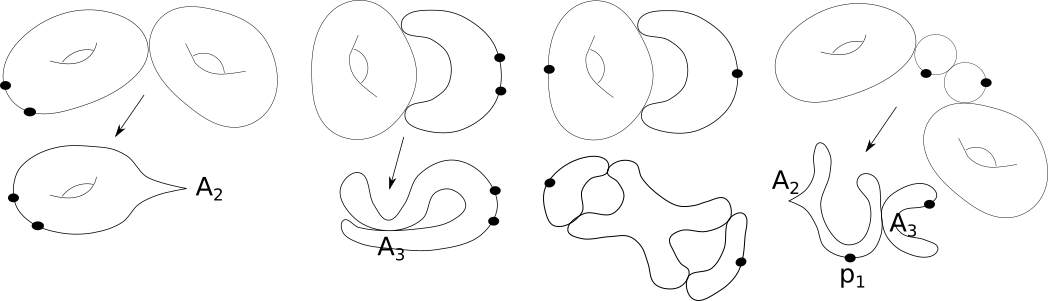
\includegraphics[width=\textwidth]{one_tail_example}
  \caption{Examples of $2$-pointed stable curves and their $1$-stable counterparts.}\label{fig:one_tail_example}
\end{figure}

We are now in a position to cast a plausible definition of $\oM_{2,2}^{(1)}$.
\begin{definition}
 A connected, reduced, complete curve of arithmetic genus two $C$ over an algebraically closed field $\k$, with smooth and disjoint markings $(p_1,p_2)$, is \emph{$1$-stable} if:
 \begin{enumerate}[leftmargin=0.7cm]
  \item $C$ has only $A_1-,\ldots,A_4-$ and dangling $A_5-$ singularities.
  %\item Every subcurve of genus two has level $2$.
  \item $C$ coincides with its minimal subcurve of arithmetic genus two.
  \item A subcurve of arithmetic genus one is either nodally attached and of level three, or it is not nodally attached and it contains $p_1$.
  %\item There is no nodally attached subcurve of genus zero.
 \end{enumerate}
\end{definition}

The main result of the paper is that $\oM_{2,2}^{(1)}$ is a proper Deligne-Mumford stack, and the generalisation of this statement to an arbitrary number of markings and a range of stability conditions that we are going to discuss in the next sections.

Let us note in passing that the birational map $\oM_{2,2}\dashrightarrow\oM_{2,2}^{(1)}$ is not defined everywhere. The reason boils down to the following
\begin{fact}
 There is only one isomorphism class of $2$-pointed curves whose normalisation is $(\PP^1,q_1)\sqcup(\PP^1,q_2,p_1,p_2)$ and having an $A_5$-singularity at $q_1=q_2$. On the other hand, the moduli space of $2$-pointed irreducible curves of geometric genus zero with an $A_4$-singularity is isomorphic to $\Aaff^1$.
\end{fact}
The second statement can be motivated as follows: the pointed normalisation of such a curve is $(\PP^1,q,p_1,p_2)$, which has neither automorphisms, nor deformations. To produce an $A_4$-singularity at $q$ we may first collapse a non-zero tangent vector at $q$ (no choice involved), producing a cusp, and then collapse a line in the tangent space at the cusp, avoiding the support of its tangent cone $\ell$ (therefore, the moduli space is $\PP^1\setminus\{\ell\}=\Aaff^1$). See Lemma \ref{lem:crimping} and the discussion thereafter.

Let $\Delta=\Delta_{2,\emptyset|0,\{1,2\}}\subseteq\oM_{2,2}$ be the divisor of rational tails, and $\mathcal W\subseteq\oM_{2,2}$ the codimension two locus of Weierstrass tails. The $1$-stable limit of any point in $\Delta\setminus\mathcal W$ is the dangling $A_5$-singularity, while the $1$-stable limit of a Weierstrass tail is ill-defined (it depends on the choice of a $1$-parameter smoothing); we conjecture that the rational map (identity on the locus of smooth curves) admits a factorisation:
\bcd
& \operatorname{Bl}_{\mathcal W}(\oM_{2,2})\ar[dl]\ar[dr] & \\
\oM_{2,2}\ar[rr,dashed] & & \oM_{2,2}^{(1)}
\ecd
The blow-up should also encode enough information to contract an unmarked elliptic bridge to a tacnode. We plan to address this point in forthcoming work.

\subsection{Relation to other work} It would be interesting to compare $\oM_{2,2}^{(1)}$ explicitly with Smyth's $\oM_{2,2}(\pazocal Z)$ \cite{SMY-towards}, for the extremal assignment $\pazocal Z$ of unmarked subcurves; here we only note that, while the divisor $\Delta_{1,\{1\}|1,\{2\}}$ is contracted in $\oM_{2,2}^{(1)}$, the latter contains a copy of $\oM_{0,4}$ (see the third column, second row of Figure \ref{fig:one_tail_example}) that is replaced by the class of the rational $4$-fold point in $\oM_{2,2}(\pazocal Z)$. $\oM_{2,2}^{(1)}$ seems closely related to the space $\pazocal U^{ns}_{2,2}(ii)$ constructed in \cite{PolishchukJohnson}. More generally, it would be interesting to relate $\oM_{2,n}^{(m)}$ (for high values of $m$) to Polishchuk's moduli of curves with nonspecial divisors \cite{Polishchuk-nonspecial}. Finally, it seems plausible that $\oM_{2,n}^{(m)}$ (for low values of $m$) corresponds to a pointed variant of the spaces of admissible hyperelliptic covers with AD singularities constructed in \cite{Fedorchuk-hyperellipticAD}.

\subsection{Outline of results and plan of the paper} In Section \ref{sec:sing} we classify all the Gorenstein curve singularities of genus two. They come in two families: the first one ($I$) includes the ramphoid cusp, the $D_5$-singularity, and for $m\geq 3$ the union of \emph{a singular branch} (a cusp) and $m-1$ lines living in $\Aaff^m$. The second one ($I\!I$) includes the $A_5$- and $D_6$-singularities, and for $m\geq 4$ the union of \emph{two tangent branches} (forming a tacnode) with $m-2$ lines in $\Aaff^{m-1}$. See Proposition \ref{prop:classification}.

In Section \ref{sec:crimp} we translate the condition that a complete pointed curve of genus two has no infinitesimal automorphisms into a \emph{mostly} combinatorial criterion. For every fixed number of branches $m$ and genus two singularity type $\in\{I,I\!I\}$, there are two isomorphism classes of pointed curves whose normalisation is $\bigsqcup_{i=1}^m(\PP^1,q_i,p_i)$ and having a singularity of the prescribed type at $q$; one of them has $\Aut(C,p)=\Gm$, while the other one has trivial automorphism group. This phenomenon is a novelty to genus two. We take a detour into moduli spaces of singularities to justify the claim, and explain how to interpret the \emph{crimping spaces} geometrically in terms of the information we need to construct a genus two singularity from a (non-Gorenstein) singularity of lower genus. This is not strictly necessary in what follows, since the singularity with one-pointed branches never satisfies the level condition we demand from our curves, yet this description is expected to be useful in analysing the indeterminacy of $\oM_{2,n}^{(m_1)}\dashrightarrow\oM_{2,n}^{(m_2)}$.

In Section \ref{sec:sstails} we study the (semi)stable limits; starting from a $1$-parameter family of semistable curves with smooth generic fibre and regular total space, we show that the shape of a subcurve of the central fibre that can be contracted into a Gorenstein singularity is strongly constrained. Singularities of type $I$ arise when the special branch (corresponding to the cusp in the contraction) is attached to a \emph{Weierstrass point} of the minimal subcurve of genus two (the \emph{core}), while singularities of type $I\!I$ occur when the special branches (corresponding to the tacnode in the contraction) are attached to \emph{conjugate points}. Furthermore, the size of the curve to be contracted only depends on one number - roughly speaking, the distance of the special branches from the core. The first statement is a consequence of the following simple observation: if $\phi\colon\widetilde{\mathcal C}\to\mathcal C$ is a contraction to a family of Gorenstein curves, $\phi^*\omega_{\mathcal C}$ is trivial on a neighbourhood of the exceptional locus of $\phi$, and it coincides with $\omega_{\widetilde{\mathcal C}}$ outside it. Now, whereas the dualising line bundle of a Gorenstein curve of genus one with no separating nodes is trivial (see \cite[Lemma 3.3]{SMY1}) and all smooth points display the same behaviour (in the sense that they are non-special), the simplest instance of Brill-Noether theory manifests itself in genus two, with the distinction between Weierstrass and non-Weierstrass points, and the expression $\omega_Z=\OO_Z(q+\sigma(q))$. The correct extension of these concepts to nodal curves was formulated in the '80s within the theory of admissible covers and limit linear series, and we spend some time to discuss the relevant combinatorics.

In Section \ref{sec:stability} we define the notion of \emph{$m$-stable} $n$-pointed curve of genus two, for every $1\leq m<n$. The basic idea is to trade worse singularities - of both genus one and two, bounded by $m$ in the sense of the embedding dimension - with more constraints on the combinatorics of the dual graph - the \emph{level} condition, which bounds below in terms of $m$ the number of special points (nodes and markings) that any subcurve of genus one or two has to contain. On the other hand, it is already clear from the discussion above that we need to break the $\mathfrak S_n$-symmetry, in order to write the dualising line bundle of the minimal subcurve of genus two as $\OO_Z(q_1+\sigma(q_1))$, in other words to choose which branches of a semistable model are to be dubbed special. We do so by using the first marking as a reference point, so that $q_1$ comes to denote the point of $Z$ closest to $p_1$. This shapes our algorithm to construct the $m$-stable limit of a given $1$-parameter smoothing. Unavoidably, the formulation of the stability condition is slightly involved, including a prescription of the interplay between $p_1$ and the singularity. We prove that the moduli stack of $m$-stable curves is algebraic, and it satisfies the valuative criterion of properness.


\subsection{Future directions of work} Besides regarding this paper as a case-study of the birational geometry of moduli spaces of curves, we are looking forwards to explore its consequences in Gromov-Witten theory. We set up some questions we would like to come back to in future work.
\begin{enumerate}[leftmargin=.7cm]
 \item The indeterminacy of the rational map $\oM_{2,n}^{(m_1)}\dashrightarrow\oM_{2,n}^{(m_2)}$ can be resolved modularly: a space dominating all the $\oM_{2,n}^{(m)}$ can be obtained as a logarithmic modification (as in \cite{RSPW1}) of the space of \emph{admissible covers} (of degree two with six ramification points). We shall describe this construction in more details in a forthcoming paper. We wonder whether the models constructed here correspond to the trace of the minimal model program on a two-dimensional slice of the cone of pseudo-effective divisors, as in \cite{SMY2}.
 
 More generally, a question outstanding to our knowledge is whether the whole program fits in the framework of stability developed in \cite{DHLinstability}.
 
 \item Applications to enumerative geometry: the link between reduced Gromov-Witten invariants in genus one (see for example \cite{VZ,Zingerred,LZ}) and maps from singular curves (see \cite{VISC}) was partially uncovered in \cite{BCM}, and brought in plain view by \cite{RSPW1,RSPW2}. In joint work with F. Carocci \cite{BC}, we exploit similar techniques to desingularise the main component of the space of genus two maps to projective space. We enrich the logarithmic structure by including a compatible admissible cover. A universal morphism to a Gorenstein curve is constructed on a logarithmically \'etale model of the base, using tools from logarithmic geometry and after choosing a \emph{tropical canonical divisor}. We stress the fact that non-reduced fibres (\emph{singular ribbons}) arise naturally in that context. The main component is recovered as those maps that factor through the Gorenstein contraction. Our desingularisation is less efficient than \cite{HLN}, but maps from singular curves provide a conceptual definition of reduced invariants for projective complete intersections and beyond. We hope that they will make comparison results (standard vs. reduced) easier to prove. This would lead to a modular interpretation of Gopakumar-Vafa invariants \cite{Pandha}.
\end{enumerate}


\section{Gorenstein curve singularities of genus two and their dualising line bundle}\label{sec:sing}

We produce an algebraic classification of the (complete) local rings of Gorenstein curve singularities of genus two over an algebraically closed field $\k$. The proof involves a technical calculation with the conductor ideal. Alternatively, one can look for a local generator of the dualising line bundle at the singularity; we remark on this below.

Let $(C,q)$ be the germ of a reduced curve singularity, and let $(R,\m)$ denote $(\hat\OO_{C,q},\m_q)$, with normalisation $(\tR,\tm)\simeq\left(\k[\![t_1]\!]\oplus\ldots\oplus\k[\![t_m]\!],\langle t_1,\ldots,t_m\rangle\right)$.
Here $m$ is the number of branches of $C$ at $q$. Recall the Definition \ref{def:genus} of the genus:
\[g=\delta-m+1;\]
so, for genus two, $\delta=m+1$. Following \cite[Appendix A]{SMY1}, we consider $\tR/R$ as a $\mathbb Z$-graded module with:
\[ (\tR/R)_i:=\tm^i/(\tm^i\cap R)+\tm^{i+1};\]
furthermore, adapting Smyth's remarks in \emph{loc. cit.} to our situation:
\begin{enumerate}
\item $m+1=\delta(p)=\sum_{i\geq 0}\dim_\k(\tR/R)_i;$
\item $2=g=\sum_{i\geq 1}\dim_\k(\tR/R)_i;$
\item\label{obs:add} if $(\tR/R)_i=(\tR/R)_j=0$ then $(\tR/R)_{i+j}=0$.
\end{enumerate}
We will also make use of the following observations:
\begin{enumerate}[resume]
 \item\label{obs:igrad} $\sum_{i\geq j}(\tR/R)_i$ is a grading of $\tm^j/(\tm^j\cap R)$;
 \item\label{obs:ses} there is an exact sequence of $R/\m=\k$-modules:
 \[ 0\to A_i:=\frac{\tm^i\cap R}{\tm^{i+1}\cap R}\to \frac{\tm^i}{\tm^{i+1}}\to \left(\tR/R\right)_i\to 0\]
\end{enumerate}
\begin{lem}\label{lem:unibranch}
 There are two unibranch curve singularities of genus two; only one of them is Gorenstein, namely the $A_4$-singularity or \emph{ramphoid cusp}: $V(y^2-x^5)\subseteq\Aaff^2_{x,y}$.
\end{lem}
\begin{proof}
 In the unibranch case $\dim_\k(\tR/R)_1\leq 1$, hence equality holds (by observation \eqref{obs:add} above). We are left with two cases:
 \begin{itemize}[leftmargin=15pt]
  \item Either $\dim_\k(\tR/R)_2=1$ and $\dim_\k(\tR/R)_i=0$ for all $i\geq 3$: in this case $\tm^3\subseteq\m$ by observation \eqref{obs:igrad}. From \eqref{obs:ses} we see that $\tm^3=\m$, hence $R\simeq\k[\![t^3,t^4,t^5]\!],$ a non-Gorenstein singularity sitting in $3$-space, which is obtained by collapsing a second-order infinitesimal neighbourhood of the origin in $\Aaff^1$ (we shall call it an ordinary cusp of genus two).
  
  \item Or $\dim_\k(\tR/R)_3=1$ and $\dim_\k(\tR/R)_i=0$ for $i=2$ and for all $i\geq 4$: in this case $\tm^4\subseteq\m$ by observation \eqref{obs:igrad}. On the other hand from $\dim_\k(\tm^2\cap R/\tm^3\cap R)=1$ we deduce that there is a generator of degree $2$, and from $\dim_\k(\tm^3\cap R/\tm^4\cap R)=0$ there is none of degree $3$. We may write the generator as $x=t^2+ct^3$, and $\m=\langle x\rangle+\tm^4$. Up to a coordinate change (i.e. automorphism of $\k[\![t]\!]$), we may take $x=t^2$, and \[\m/\m^2=\langle t^2,t^5\rangle,\] so $R\simeq\k[\![x,y]\!]/(x^5-y^2)$, as anticipated.
 \end{itemize}
\end{proof}

From now on, we only look for Gorenstein singularities. With notation as above, let $I=(R:\tilde R)=\operatorname{Ann}_R(\tilde R/R)$ be the \emph{conductor ideal} of the singularity. Recall e.g. \cite[Proposition VIII.1.16]{AK}: $(C,q)$ is Gorenstein if and only if
\[\dim_\k(R/I)=\dim_\k(\tR/R)(=\delta).\]

Recall from \cite[Definition 2-1]{Stev} that a curve singularity $(C,q)$ is \emph{decomposable} if $C$ is the union of two curves $C_1$ and $C_2$ that lie in distinct smooth spaces intersecting each other transversely in $q$. Given a parametrisation $x_i=x_i(t_1,\ldots,t_m),\ i=1,\ldots,l$, this means that there is a partition $S\sqcup S^\prime=\{1,\ldots,m\}$ such that $x_i$ only depends on $t_s,s\in S$, or $s\in S^\prime$, for all $i$. Aside from the node, Gorenstein singularities are never decomposable \cite[Proposition 2.1]{AFSGm}.

\begin{prop}\label{prop:classification}
 For every fixed integer $m\geq 2$, there are exactly two Gorenstein curve singularities of genus two with $m$ branches.
\end{prop}
\begin{proof}
 We only need to find a basis for $\m/\m^2$, because a map of complete local rings that is surjective on cotangent spaces is surjective. From observation \eqref{obs:add} again, we find three possibilities for the vector $(d_1,d_2,d_3)$, $d_i=\dim_{\k}(\tR/R)_i$; $d_{\geq 4}=0$ in any case.
 
 \smallskip
 
 \textbf{Case} $(2,0,0)$. We see that $\tm^2\subseteq I$, so, if $(C,q)$ were Gorenstein, \eqref{obs:ses} would imply: \[m+1=\delta=\dim_\k(R/I)\leq \dim_\k(R/\tm^2)=\dim_\k A_0+\dim_\k A_1=1+(m-2)=m-1,\] a contradiction. Note: the singularity turns out to be decomposable in this case.
 
 \smallskip
 
 \textbf{Case} $(1,1,0)$. We have $\tm^3\subseteq I$. We are going to write down the $m-1$ generators of $A_1 \pmod {\tm^3}$\footnote{To express them in the simplest possible form, we perform at first only polynomial manipulations of the generators, while changing coordinates on the normalisation only at the end - the benefit of this two-step process will become apparent in the next section.}. The first generator, call it $x_1$, has a non-trivial linear term in at least one of the variables, say $t_1$. By scaling $x_1$ and possibly adding a multiple of $x_1^2$, we can make it into the form:
 $x_1=t_1\oplus p_{1,2}(t_2)\oplus\ldots\oplus p_{1,m}(t_m) \pmod{\tm^3}.$ Now we can use $x_1$ and $x_1^2$ to make sure the second generator does not involve $t_1$ at all. It will still have a linear term independent of $t_1$, say non-trivial in $t_2$. By scaling and adding a multiple of $x_2^2$, we can write $x_2=0\oplus t_2\oplus\ldots\oplus p_{2,m}(t_m) \pmod{\tm^3}.$ By taking a linear combination of $x_1$ with $x_2$ and $x_2^2$, we may now reduce $x_1$ to the form $t_1\oplus0\oplus p_{1,3}(t_3)\oplus\ldots\oplus p_{1,m}(t_m)\pmod{\tm^3}$. Continuing this way, by Gaussian elimination with the generators and their squares, we may write them as:
 \begin{align*}
  x_1= & t_1\oplus0\oplus\ldots\oplus\alpha_{1,m}t_m+\beta_{1,m}t_m^2\\
  x_2= & 0\oplus t_2\oplus\ldots\oplus\alpha_{2,m}t_m+\beta_{2,m}t_m^2\\
  &\ldots\\
  x_{m-1}= & 0\oplus\ldots\oplus t_{m-1}\oplus\alpha_{m-1,m}t_m+\beta_{m-1,m}t_m^2 \pmod{\tm^3}.
 \end{align*}
 If $x_i\in I$ for some $i$, then $t_i\in R$, and the singularity would be decomposable. So, by the Gorenstein condition, $R/I$ is generated by $1,x_1,\ldots,x_{m-1},$ and an extra element $y$. Hence $x_i^2\in I$ for all but at most one $i$, say $i=1$. Then $t_i^2\in R$ for $i=2,\ldots,m-1$. If $\alpha_{i,m}\neq 0$ for some $i$ in this range, then $t_m^2\in R$ as well, so $t_1^2=x_1^2-O(t_m^2)\in R$, contradicting $\dim_\k(\tR/R)_2=1$. Therefore $\alpha_{i,m}=0$ for $i\in\{2,\ldots,m-1\}$. If $\alpha_{1,m}=0$, there would be another generator of $\m/\m^2$, that could be taken to be $z=0\oplus\ldots\oplus t_m^3$. In this case, though, both $x_1^2$ and $z$ would belong to $I$, so $\dim_k(R/I)=m$, and the singularity could not be Gorenstein. We are reduced to the following expression:
 \begin{align}\label{coordII-cs}
 \begin{split}
  x_1= & t_1\oplus0\oplus\ldots\oplus\alpha_{1,m}t_m+\beta_{1,m}t_m^2\\
  x_2= & 0\oplus t_2\oplus\ldots\oplus\beta_{2,m}t_m^2\\
  &\ldots\\
  x_{m-1}= & 0\oplus\ldots\oplus t_{m-1}\oplus \beta_{m-1,m}t_m^2 \pmod{\tm^3},
 \end{split}
 \end{align}
 with $\beta_{1,m}\in\k$ and $\alpha_{1,m},\beta_{i,m}\in\k^\times,\ i=2,\ldots,m-1$ (by indecomposability). Finally, we change coordinates in $t_m$ (abusing notation, $t_m:=\alpha_{1,m}t_m+\beta_{1,m}t_m^2$) and rescale the other $t_i$ to obtain:
 \begin{align}\label{coordII}
 \begin{split}
  x_1= & t_1\oplus0\oplus\ldots\oplus t_m\\
  x_2= & 0\oplus t_2\oplus\ldots\oplus t_m^2\\
  &\ldots\\
  x_{m-1}= & 0\oplus\ldots\oplus t_{m-1}\oplus t_m^2\pmod{\tm^3}.
 \end{split}
 \end{align}
 We check that $R/I=\langle 1,x_1,\ldots,x_{m-1},x_1^2\rangle$ and $\tR/R$ is of type $(1,1,0)$. In case $m=2$, we need an extra generator $y=t_2^3$. Equations are given by:
 \begin{itemize}
  \item $y(y-x_1^3)$ if $m=2$ ($A_5$-singularity or \emph{oscnode});
  \item $x_1x_2(x_2-x_1^2)$ if $m=3$ ($D_6$-singularity);
  \item $\langle x_3(x_1^2-x_2),x_i(x_j-x_k)\rangle_{1\leq i<j<k\leq m-1 \text{ or }1<j<k<i\leq m-1}$ if $m\geq 4$.
 \end{itemize}

 \smallskip
 
 \textbf{Case} $(1,0,1)$. We have $\tm^4\subseteq I$. By an argument similar to the above one, we write generators for $A_1$ as $x_i=\ldots\oplus t_i\oplus\ldots \oplus\alpha_{i,m}t_m+\beta_{i,m}t_m^2+\gamma_{i,m}t_m^3$, for $i=1,\ldots,m-1$.
 Then $R/I=\langle 1,x_1,\ldots,x_{m-1},y\rangle$. For all but at most one $i$, $x_i^2\in I$, but definitely $x_i^3\in I$ for all $i$. On the other hand $t_m^3\notin R$, because otherwise $t_i^3=x_i^3-\alpha_{i,m}^3t_m^3+O(t_m^4)$ would belong to $R$ as well, contradicting $\dim_\k(\tR/R)_3=1$. From this we deduce that $\alpha_{i,m}=0$ for all $i=1,\ldots,m-1$. Since $\dim_\k(\tR/R)_2=0$, there has to be another generator of $\m/\m^2$ of degree two in $t_m$, which we may write as $x_m=t_m^2+\gamma_{m,m}t_m^3$. We can use $x_m$ to remove all the $t_m^2$ pieces from $x_1,\ldots,x_{m-1}$, so we are reduced to the following expression:
  \begin{align}\label{coordIII-cs}
 \begin{split}
  x_1= & t_1\oplus0\oplus\ldots\oplus \gamma_{1,m}t_m^3\\
  x_2= & 0\oplus t_2\oplus\ldots\oplus \gamma_{2,m}t_m^3\\
  &\ldots\\
  x_{m-1}= & 0\oplus\ldots\oplus t_{m-1}\oplus \gamma_{m-1,m}t_m^3\\
  x_m= & 0\oplus\ldots\oplus t_m^2+\gamma_{m,m}t_m^3 \pmod{\tm^4},
  \end{split}
 \end{align}
 with $\gamma_{m,m}\in\k$ and $\gamma_{i,m}\in\k^\times,\ i=1,\ldots,m-1$ (by indecomposability). Finally, we change coordinates in $t_m$ (abusing notation $t_m:=t_m\sqrt{1+\gamma_{m,m}t_m}$)\footnote{For this to be possible, we have to assume that $\k$ has characteristic different from $2$.} and rescale the other $t_i$ to obtain:
 \begin{align}\label{coordIII}
 \begin{split}
  x_1= & t_1\oplus0\oplus\ldots\oplus t_m^3\\
  x_2= & 0\oplus t_2\oplus\ldots\oplus t_m^3\\
  &\ldots\\
  x_{m-1}= & 0\oplus\ldots\oplus t_{m-1}\oplus t_m^3\\
  x_m= & 0\oplus\ldots\oplus t_m^2 \pmod{\tm^4}.
  \end{split}
 \end{align}
 We check that $R/I=\langle 1,x_1,\ldots,x_{m-1},x_m\rangle$ and $\tR/R$ is of type $(1,0,1)$. Incidentally, when $m=1$, we recover the unique Gorenstein singularity of Lemma \ref{lem:unibranch}. Equations are given by:
 \begin{itemize}
  \item $x^5-y^2$ if $m=1$ ($A_4$-singularity or \emph{ramphoid cusp}, with $x=t^2,y=t^5$);
  \item $y(y^3-x^2)$ if $m=2$ ($D_5$-singularity, with $x=x_1,y=x_2$);
  \item $\langle x_3(x_1-x_2),x_3^3-x_1x_2\rangle$ if $m=3$;
  \item $\langle x_i(x_j-x_k), x_m(x_i-x_j),x_m^3-x_1x_2\rangle_{i,j,k\in\{1,\ldots,m-1\}\text{ all different}}$ if $m\geq 4$.
 \end{itemize}
\end{proof}

%\begin{rem}
 %Not-necessarily Gorenstein singularities can be obtained by gluing various Gorenstein singularities of genus $\leq 2$ along subschemes of length $\leq 3$. Classifying all of them would not necessarily be easy.
%\end{rem}

\begin{rem}
 We sketch an alternative proof of the above proposition based on meromorphic differentials, see also Corollary \ref{cor:dualising_line_bundle} below. We address the case $(1,0,1)$ and leave the (easier) case $(1,1,0)$ to the interested reader. The setup is as in \cite[\S 2.1]{RSPW2}: let $C$ be a projective Gorenstein curve with a unique singularity of genus two at the point $q$. Let:
 \[ \widetilde C\xrightarrow{\nu}\widehat C\xrightarrow{\mu} C\]
 be respectively the normalisation and semi-normalisation of $C$. We have inclusions:
 \begin{align*}
  {} & \OO_C & \subseteq & \mu_* \OO_{\widehat C} & \subseteq & \mu_*\nu_* \OO_{\widetilde C} & \subseteq K \\
  J  \supseteq & \omega_C & \supseteq & \mu_* \omega_{\widehat C} & \supseteq & \mu_*\nu_* \omega_{\widetilde C}
 \end{align*}
where $K$ is the sheaf of rational functions, and $J$ the sheaf of meromorphic differentials. The rows are dual to each other with respect to the residue pairing $J\otimes K\to\k$ \cite[Proposition 1.16(ii)]{AK}. The skyscraper sheaf $\omega_{\widehat C}/\nu_* \omega_{\widetilde C}$ is generated by the logarithmic differentials:
\begin{equation}\label{eqn:logdifferentials}\frac{\operatorname{d} t_i}{t_i}-\frac{\operatorname{d} t_j}{t_j},\quad i,j\in\{1,\ldots,m\}.\end{equation}
The skyscraper sheaves $\mu_*\OO_{\widehat C}/\OO_C$ and $\omega_C/\mu_*\omega_{\widehat C}$ have length two. Let $\eta_1$ be a generator of the latter; since $C$ is Gorenstein, we may assume that $\eta_1$ is a local generator of $\omega_C$. Since $\tm^4\subseteq R$ and by Equation \eqref{eqn:logdifferentials}, we may assume that $\eta_1$ takes the following form:
\begin{equation}\label{eqn:eta1}\eta_1=\zeta\frac{\operatorname{d} t_1}{t_1}+\sum_{i=1}^m \alpha_i \frac{\operatorname{d} t_i}{t_i^2}+ \sum_{i=1}^m \beta_i \frac{\operatorname{d} t_i}{t_i^3}+ \sum_{i=1}^m \gamma_i \frac{\operatorname{d} t_i}{t_i^4}.\end{equation}
Since the constant functions descend to $C$, the residue condition implies that $\zeta=0$. Now, $\mu_*\omega_{\widehat C}/\omega_C$ has a second generator $\eta_2$ of the form $\eta_2=f\eta_1$ for some $f\in R$. Expanding $f=f_0+\sum_{i,j}f_{i,j}t_i^j$ we may write:
\begin{equation}\label{eqn:eta2}
 \eta_2=\sum_{i=1}^m(\beta_if_{i,1}+\gamma_if_{i,2})\frac{\operatorname{d} t_i}{t_i^2}+\sum_{i=1}^m\gamma_if_{i,1}\frac{\operatorname{d} t_i}{t_i^3}.
\end{equation}
Not all the $\gamma_i$ can be zero, otherwise we would have $\tm^3\subseteq R$, so say $\gamma_m\neq 0$; this implies that $t_m^3\notin R$ (and in particular $t_m\notin R$). Up to scaling we have $\gamma_m=1$. Since $A_3$ has dimension one, for every $i=1,\ldots,m-1$ there is a linear combination:
\[ g_i=t_i^3+x_it_m^3\in R.\]
Pairing with $\eta_1$ we find $x_i=-\gamma_i$.

Since $A_2=0$, for every $i=1,\ldots,m$ there is a linear combination:
\[ h_i=t_i^2+y_it_m^3\in R.\]
Pairing with $\eta_1$ we find $y_i=-\beta_i$. Pairing with $\eta_2$ we find $\gamma_if_{i,1}=0$ (so $f_{m,1}=0$). Equation \eqref{eqn:eta2} becomes:
\[\eta_2=\left(\sum_{i:\gamma_i=0,f_{i,1}\neq 0}\beta_if_{i,1}+\sum_{i:\gamma_i\neq0,f_{i,1}=0}\gamma_if_{i,2}\right)\frac{\operatorname{d} t_i}{t_i^2}.\]

Since $A_1$ has dimension one and $t_m\notin R$, for every $i=1,\ldots,m-1$ there is a linear combination:
\[ l_i=t_i+z_it_m^3\in R.\]
Pairing with $\eta_1$ we find $z_i=-\alpha_i$. So $\alpha_i\neq0$ for $i=1,\ldots,m-1$, otherwise $C$ would be decomposable. Pairing with $\eta_2$ we find
\begin{equation}\label{eqn:someequation}\beta_if_{i,1}+\gamma_if_{i,2}=0,\qquad i=1,\ldots,m-1.\end{equation}
Taking $l_i^2$, we have $t_i^2\in R, i=1,\ldots,m-1,$ as well. Pairing with $\eta_1$, we find $\beta_i=0$.

\noindent Taking $l_i^3$, we have $t_i^3\in R, i=1,\ldots,m-1,$ as well. Pairing with $\eta_1$, we find $\gamma_i=0$. So, ultimately, we find:
\[\eta_2=\frac{\operatorname{d} t_m}{t_m^2}.\]
By taking a linear combination with $\eta_2$, Equation \eqref{eqn:eta1} becomes:
\[\eta_1=\sum_{i=1}^{m-1} \alpha_i \frac{\operatorname{d} t_i}{t_i^2}+ \beta_m \frac{\operatorname{d} t_m}{t_m^3}+  \frac{\operatorname{d} t_m}{t_m^4}, \text{ with } \alpha_i\in\k^\times,\beta_m\in\k.\]
\end{rem}

\begin{definition}\label{def:special_branches}
 In case $(1,0,1)$, we say the singularity is \emph{of type $I$}, and the branch parameterised by $t_m$ is called \emph{singular}; in case $(1,1,0)$, we say the singularity is \emph{of type $I\!I$}, and the branches parameterised by $t_1$ and $t_m$ are called \emph{twin}. We shall refer to the singular or twin branches as \emph{special} or \emph{distinguished}; all other branches are \emph{axes}. \emph{Branch} remains a generic name, indicating any of the previous ones.
\end{definition}

We gather a description of the dualising line bundle in the following:
\begin{cor}\label{cor:dualising_line_bundle}
 Let $\nu\colon C\to \bar C$ be the normalisation of a Gorenstein singularity of genus two, with $\nu^{-1}(q)=\{q_1,\ldots,q_m\}$.
 \begin{enumerate}[label=(\Roman*)]
 
 \item With local parametrisation as in \eqref{coordIII}, $\omega_{\bar C}$ is generated by: \[\frac{\operatorname{d}t_1}{t_1^2}+\ldots+\frac{\operatorname{d}t_{m-1}}{t_{m-1}^2}-\frac{\operatorname{d}t_m}{t_m^4},\]
 and $\nu^*\omega_{\bar C}=\omega_C(2q_1+\ldots+2q_{m-1}+4q_m)$.

 \item With local parametrisation as in \eqref{coordII}, $\omega_{\bar C}$ is generated by:
  \[\frac{\operatorname{d}t_1}{t_1^3}+\frac{\operatorname{d}t_2}{t_2^2}+\ldots+\frac{\operatorname{d}t_{m-1}}{t_{m-1}^2}-\frac{\operatorname{d}t_m}{t_m^3},\]  
  and $\nu^*\omega_{\bar C}=\omega_C(3q_1+2q_2+\ldots+2q_{m-1}+3q_m)$.
                                                                                                                                  \end{enumerate}
\end{cor}

\begin{rem}
 Singularities of type $I$ do appear in the miniversal family of singularities of type $I\!I$, and vice versa. For low values of $m$, this follows from a neat result of Grothendieck (\cite[p. 2277]{C-ML}, see also \cite{Arnold,Demazure}):
 \begin{thm}\label{thm:ADE}
  Let $(C,q)$ be a curve singularity of ADE type. The singularities appearing in the miniversal deformation of $(C,q)$ are all and only the ADE singularities whose Dynkin diagram can be obtained as a full subgraph of the Dynkin diagram of $(C,q)$.
 \end{thm}
\end{rem}


\section{Tangent sheaf, crimping space, and automorphisms}\label{sec:crimp}
In this section we analyse the tangent sheaf of a genus two singularity. For a complete pointed Gorenstein curve of genus two, we translate the absence of infinitesimal automorphisms into a (mostly) combinatorial criterion. We will use this in Section \ref{sec:stability}, when we define stability conditions on the stack of pointed Gorenstein curves of genus two, to make sure that the resulting substacks are Deligne-Mumford. The crimping space naturally makes an appearance. Although we do not use it explicitly in this paper, it parametrises singularities of a given type and pointed normalisation. It helps understanding the birational map between two compactifications of $\pazocal{M}_{2,n}$.

In the next lemma, we find explicit conditions for a vector field on the normalisation, vanishing at the preimage of the singular point, to descend to the singular curve.

\begin{lem}\label{lem:aut}
Let $(C,q)$ be a Gorenstein curve singularity of genus two, with pointed normalisation $\nu\colon(\tilde C,\{q_i\}_{i=1,\ldots,m})\to (C,q)$, and assume $\operatorname{char}(\k)\neq 2,3$. There are exact sequences of sheaves
\bcd
0\ar[r]  & \nu_*\Omega_{\tilde C}^\vee(-\sum_i 3q_i)\ar[r]  &\nu_*\Omega_{\tilde C}^\vee(-\sum_i q_i)\ar[r]\ar[dr,phantom,"\Box"]  &\nu_*\bigoplus_i\Omega_{\tilde C}^\vee(-q_i)_{|2q_i}\ar[r]  & 0 \\
0\ar[r]  &\nu_*\Omega_{\tilde C}^\vee(-\sum_i 3q_i)\ar[r]\ar[u,equal]  & \Omega_C^\vee\ar[r]\ar[u] & \k^{\oplus m}\ar[r]\ar[u,hook,"\phi"] & 0
\ecd
 The image of the rightmost vertical map admits an explicit description in local coordinates.
\end{lem}
\begin{proof}
 Let $K(\tilde C)$ denote the locally constant sheaf of rational functions on $\tilde C$. A section of $\Omega_{\tilde C}^\vee\otimes K(\tilde C)$ is contained in $\Omega_C^\vee$ if and only if its image under the push-forward map:
 \[\nu_*\colon\nu_*\hhom(\Omega_{\tilde C},K(\tilde C))\to \hhom(\Omega_C,K(\tilde C)) \]
 lies in the subspace $\hhom(\Omega_C,\OO_C)$. Since in any case $\widetilde{\mathfrak m}^4\subseteq\mathfrak m$ (see the proof of Proposition \ref{prop:classification}), vector fields vanishing up to order three certainly descend. In order to find the remaining conditions, we may work locally around the singular point in the coordinates of Section \ref{sec:sing}.
\begin{description}[leftmargin=0pt]
 \item[$(A_4):$] In the coordinates $x=t^2+ct^3,y=t^4,z=t^5$ (they are redundant, but this will be irrelevant), the section $f(t)\frac{d}{dt}\in\nu_*\Omega_{\tilde C}^\vee\otimes K(\tilde C)$ pushes forward to
 \[\nu_*\left(f(t)\frac{d}{dt}\right)=(2t+3ct^2)f(t)\frac{d}{dx}+4t^3f(t)\frac{d}{dy}+5t^4f(t)\frac{d}{dz},\]
 from which, writing $f(t)=f_0+f_1t+f_2t^2+O(t^3)$, we see that
 \[(2t+3ct^2)f(t),4t^3f(t),5t^4f(t)\in\hat\OO_{C,p}\Leftrightarrow f_0=0,cf_1+2f_2=0.\]
 
 \item[$(A_5):$] In the coordinates $x=t_1\oplus at_2+bt_2^2,y=t_1^3$ (we have $a\neq 0$), the section $f_1(t_1)\frac{d}{dt_1}\oplus f_2(t_2)\frac{d}{dt_2}$ pushes forward to
 \[\nu_*\left(f_1(t_1)\frac{d}{dt_1}\oplus f_2(t_2)\frac{d}{dt_2}\right)=\left(f_1(t_1)\oplus (a+2bt_2) f_2(t_2)\right)\frac{d}{dx}+3t_1^2f_1(t_1)\frac{d}{dy},\]
 from which, writing $f_i(t_i)=f_{i0}+f_{i1}t_i+f_{i2}t_i^2+O(t_i^3),i=1,2$, we see that
 \[f_1(t_1)\oplus (a+2bt_2)f_2(t_2),3t_1^2f_1(t_1)\in\hat\OO_{C,p} \Leftrightarrow \begin{cases} f_{10}=f_{20}=0,\\ f_{11}=f_{21},\\ 2bf_{21}+af_{22}=a^2f_{12}.\end{cases}\]
 
  \item[$(I_{m\geq 2}):$] In the coordinates of \eqref{coordIII-cs},
 \[\nu_*\left(\sum_{i=1}^m f_i(t_i)\frac{d}{dt_i}\right)=\sum_{i=1}^{m-1}\left(f_i(t_i)\oplus3\gamma_{i,m}t_m^2f_m(t_m)\right)\frac{d}{dx_i}+\\(2t_m+3\gamma_{m,m}t_m^2)f_m(t_m)\frac{d}{dx_m},\]
 hence we deduce that
 \[\nu_*\left(\sum_{i=1}^m f_i(t_i)\frac{d}{dt_i}\right)\in\Omega_C^\vee\otimes\hat\OO_{C,p}\Leftrightarrow \begin{cases} f_{i0}=0 & i=1,\ldots,m,\\ f_{i1}=3f_{m1}, & i=1,\ldots,m-1,\\ 3\gamma_{m,m}f_{m1}+2f_{m2}=0.\end{cases}\]
 
 \item[$(I\!I_{m\geq 3}):$] In the coordinates of \eqref{coordII-cs},
 \begin{multline*}\nu_*\left(\sum_{i=1}^m f_i(t_i)\frac{d}{dt_i}\right)=\left(f_1(t_1)\oplus(\alpha_{1,m}+2\beta_{1,m}t_m) f_m(t_m)\right)\frac{d}{dx_1}+\\
 \sum_{i=2}^m\left(f_i(t_i)\oplus2\beta_{i,m}t_mf_m(t_m)\right)\frac{d}{dx_i},\end{multline*}
 hence we deduce that
 \[\nu_*\left(\sum_{i=1}^m f_i(t_i)\frac{d}{dt_i}\right)\in\Omega_C^\vee\otimes\hat\OO_{C,p}\Leftrightarrow \begin{cases} f_{i0}=0 & i=1,\ldots,m,\\ 2f_{11}=f_{i1}=2f_{m1}, &  i=2,\ldots,m-1,\\ \beta_{1,m}f_{m1}+\alpha_{1,m}f_{m2}=\alpha_{1,m}^2f_{12}.\end{cases}\]
 
\end{description}
\end{proof}

We anticipate that the letters $\alpha,\beta$ and $\gamma$ will play a role in determining the automorphism group of a complete curve with markings. We recall some key concepts from F. van der Wyck's thesis.
Working over $\k$, he considers the stacks:
\begin{itemize}[leftmargin=.5cm]
 \item $\mathcal S$ of reduced one-dimensional (1d) $\k$-algebras $R$,
 \item $\mathcal T$ of reduced 1d algebras with resolution $(R\hookrightarrow (S,J))$, where $S$ is a smooth one-dimensional $\k$-algebra, and $J$ the radical of the conductor of $R\subseteq S$.
\end{itemize}
  Basically, $R$ represents the (local) ring of a reduced curve with one singular point, $S$ is its normalisation, and $J$ is the ideal of the reduced fibre over the singular point of $\operatorname{Spec}(R)$. $\mathcal S$ and $\mathcal T$ are limit-preserving stacks over $\operatorname{Spec}(\k)$ \cite[Proposition 1.21]{vdW}. Furthermore, we may fix a reduced 1d algebra with resolution $\tau_0:(R_0\hookrightarrow(S_0,J_0))$, and consider the substack $\mathcal T(\tau_0)$ of reduced 1d algebras with singularity type $\tau_0$ (i.e. isomorphic to $\tau_0$ locally on both the base and the curve, see \cite[Definition 1.64]{vdW}; that various notions of ``locally'' coincide is proved in \cite[Proposition 1.50]{vdW}). There is a forgetful morphism $\mathcal T\to\mathcal S$, and the \emph{crimping space} of $\tau_0$ is defined to be the fibre over $R_0$ of the restriction of such morphism to $\mathcal T(\tau_0)$. The crimping space is a smooth $\k$-scheme \cite[Theorems 1.70 and 1.73]{vdW}; indeed, it is isomorphic to the quotient of $\Aut_{(S_0,J_0)/\k}$ by $\Aut_{(S_0,J_0)/R_0}$, the latter consisting of automorphisms of the normalisation that preserve the subalgebra of the singularity; moreover, by \cite[Theorem 1.53]{vdW} the quotient can be computed after modding out the lowest power of $J$ contained in $R$, denoted by $\Aut_{(S,J)}^{\mod J^k}$ respectively $\Aut_{(S,J)/R}^{\mod J^k}$. Crimping spaces can be thought of as moduli for the normalisation map.
  
\begin{lem}\label{lem:crimping}
 If $\operatorname{char}(\k)\neq2,3$, the crimping space of a genus two singularity of type $I$ (resp. $I\!I$) with $m$ branches is the disjoint union of $m$ (resp. ${m}\choose{2}$) copies of $\Aaff^1\times(\Aaff^1\setminus\{0\})^{m-1}$.
\end{lem}
\begin{proof}
We resume notation from the previous section. We are going to fix the subalgebra $\tau_0$ given in coordinates by \eqref{coordIII} and \eqref{coordII} respectively.

\textbf{Type $I$}: recall that in this case $\tm^4\subseteq R$. For a $\k$-algebra $A$, let
\[G_i(A)=\{t_i\mapsto g_{i1}t_i+g_{i2}t_i^2+g_{i3}t_i^3,t_j\mapsto t_j\ |\ g_{i1}\in A^\times,g_{i2},g_{i3}\in A\},\]
and notice that
\[\Aut_{(\tR,\tm)}^{\mod\tm^4}(A)=(G_1\times\ldots\times G_m)\rtimes \mathfrak{S}_m(A).\]

Consider now the action of a group element of the form $(g_1,\ldots,g_m;\id_{\mathfrak{S}_m})$ on the given generators of $R$:
\begin{align*}
 x_i\mapsto& \ldots\oplus g_{i1}t_i+g_{i2}t_i^2+g_{i3}t_i^3\oplus\ldots\oplus g_{m1}^3t_m^3,\quad\text{for } i=1,\ldots,m-1;\\
 x_m\mapsto& \ldots\oplus g_{m1}^2t_m^2+2g_{m1}g_{m2}t_m^3 \pmod{\tm^4}.
\end{align*}
The former belongs to $R$ iff $g_{i1}=g_{m1}^3$; the latter does iff $g_{m2}=0$. Thus such elements span a subgroup isomorphic to $\Gm\times\Ga^{m-1}\times\Ga^m(A)$. On the other hand, there is a special (singular) branch, parametrised by $t_m$. We conclude that
\[\Aut_{\tau_0}^{\mod\tm^4}(A)=(\Gm\times\Ga^{m-1}\times\Ga^m)\rtimes(\mathfrak{S}_{m-1})(A).\]
The quotient is therefore isomorphic to $m$ copies of $\Aaff^1\times(\Aaff^1\setminus\{0\})^{m-1}$. 

\textbf{Type $I\!I$}: recall that in this case $\tm^3\subseteq R$. For a $\k$-algebra $A$, let
\[G_i(A)=\{t_i\mapsto g_{i1}t_i+g_{i2}t_i^2,t_j\mapsto t_j\ |\ g_{i1}\in A^\times,g_{i2}\in A\},\]
and notice that
\[\Aut_{(\tR,\tm)}^{\mod\tm^3}(A)=(G_1\times\ldots\times G_m)\rtimes \mathfrak{S}_m(A).\]

Consider now the action of a group element of the form $(g_1,\ldots,g_m;\id_{\mathfrak{S}_m})$ on the given generators of $R$:
\begin{align*}
 x_i\mapsto& \ldots\oplus g_{i1}t_i+g_{i2}t_i^2\oplus\ldots\oplus g_{m1}^2t_m^2,\quad\text{for } i=2,\ldots,m-1;\\
 x_1\mapsto& g_{11}t_1+g_{12}t_1^2\oplus\ldots\oplus g_{m1}t_m+g_{m2}t_m^2 \pmod{\tm^3}.
\end{align*}
The former belongs to $R$ iff $g_{11}=g_{m1}$ and $g_{12}=g_{m2}$; the latter does iff $g_{i1}=g_{m1}^2$. Thus, such elements span a subgroup isomorphic to $\Gm\times\Ga^{m-1}(A)$. On the other hand, all branches are smooth (therefore, isomorphic to each other), but two of them (parametrised by $t_1$ and $t_m$ respectively) are tangent, thus forming a distinguished pair. We conclude that
\[\Aut_{\tau_0}^{\mod\tm^3}(A)=(\Gm\times\Ga^{m-1})\rtimes(\mathfrak{S}_2\times\mathfrak{S}_{m-2})(A).\]
The quotient is then isomorphic to $\binom{m}{2}$ copies of $\Aaff^1\times(\Aaff^1\setminus\{0\})^{m-1}$.
\end{proof}


\begin{rem}
 The restrictions on the characteristic of the base field in Lemmas \ref{lem:aut} and \ref{lem:crimping} rule out the sporadic occurrence of infinite families of automorphisms, and its effect on the crimping spaces. For example, when $\operatorname{char}(\k)=2$, the singularities $\k[\![t^2,t^5]\!]$ and $\k[\![t^2+t^3,t^4,t^5]\!]$ are not isomorphic, the group of infinitesimal automorphisms has positive dimension, and the crimping space consists of an isolated point \cite[Examples 1.79-80]{vdW}.
\end{rem}

The benefit of a two-step classification should now be clear: if we do not allow ourselves to change coordinates (i.e. act by automorphisms of the normalisation) until the end, the crimping space appears in the expressions \eqref{coordII-cs} and \eqref{coordIII-cs} for the generators of the singularity subalgebra.


There is a more geometric way to realise the crimping spaces. It is well-known that an ordinary cusp of genus one can be obtained by collapsing (\emph{push-out}) any non-zero tangent vector at $p\in\Aaff^1$. More generally, a Gorenstein singularity of genus one and $m$ branches can be obtained by collapsing a generic (not contained in any coordinate linear subspace) tangent line at an ordinary $m$-fold point (a non-Gorenstein singularity of genus zero) \cite[Lemma 2.2]{SMY1}. Therefore, the crimping space of the elliptic $m$-fold point, which is isomorphic to $(\Aaff^1\setminus\{0\})^{m-1}$, can be realised as the complement of the coordinate hyperplanes inside $\PP(T_pR_m)\simeq\PP^{m-1}$, where $(R_m,p)$ is the rational $m$-fold point. Besides, this gives rise to a natural compactification of the crimping space supporting a universal family of curves - in fact, two: either we collapse non-generic tangent vectors, obtaining non-Gorenstein singularities along the boundary (this family $\mathcal C$ admits a common (semi)normalisation by the trivial family $\widetilde{\mathcal C}=R_m\times \PP(T_pR_m)$); or we blow $\widetilde{\mathcal C}$ up along the boundary (\emph{sprouting}), so that the non-Gorenstein singularities are replaced by elliptic $m$-fold points having strictly semistable branches \cite[\S 2.2-3]{SMY2}.

Similarly, a Gorenstein singularity of genus two can be obtained by collapsing a generic line in the tangent space of a non-Gorenstein singularity of genus one. Indeed, $\tau_0^{I}$ admits a partial normalisation by $\sigma_0^{I}$, which is the decomposable union of a cusp (parametrised by $t_m$) together with $m-1$ axes; the local ring of $\sigma_0^{I}$ is obtained from that of $\tau_0^{I}$ by adjoining the generator $t_m^3$.  $\tau_0^{I\!I}$ admits a partial normalisation by $\sigma_0^{I\!I}$, which is the decomposable union of a tacnode in the $(t_1,t_m)$-plane together with $m-2$ axes, adjoining the generator $t_m^2$.

These fit together nicely in a unifying picture: if we restrict $\mathcal C$ from the previous paragraph to the union of the coordinate lines in $\PP(T_pR_m)$, we obtain $m$ copies of $\sigma_0^{I}$ over the coordinate points, together with $\binom{m}{2}$ copies of the universal curve of type $\sigma_0^{I\!I}$ over its crimping space - which is isomorphic to $\Aaff^1\setminus\{0\}$ - identified with the line minus two points. Let $P=\PP(T_{\mathcal C/\PP,p|\cup\text{lines}})$ be the projectivised tangent space of the fibre at the singular point. For each of the $\binom{m}{2}$ coordinate lines, $P$ has one component $P^{I\!I}_i$ that is a $\PP^{m-1}$-bundle over the line; besides, $P$ has $m$ components $P^{I}_j$ isomorphic to $\PP^m$ and supported over the points. The crimping space of the genus two singularities with $m$ branches (of type $I$ and $I\!I$ together) can be realised as an open subscheme of $P$, obtained by removing from the $\PP^{m-1}$-fibres of $P^{I\!I}$ the $m-1$ hyperplanes generated by (a) the tangent line to the tacnode and the $m-2$ axes, and (b) the plane containing the tacnode and all but one of the $m-2$ axes; and from each $P^{I}_j$ the $m$ planes generated by (a) the tangent cone of the cusp and the $m-1$ axes, and (b) the plane containing the cusp and all but one of the $m-1$ axes.

\begin{rem}
 Crimping spaces are related to the space of arrows $\phi$ in the diagram of Lemma \ref{lem:aut}.
 
 We interpret $H^0(\Omega_{\PP^1}^\vee(-p)_{|2p})$ as the tangent space to the subgroup of $PGL_2$ fixing the point $p\in\PP^1$, thus it inherits a natural Lie algebra structure, isomorphic to the unique non-abelian Lie algebra of dimension two $V$. It has a basis: \[e_1=\begin{pmatrix} 1 & 0 \\ 0 & -1\end{pmatrix}, \quad e_2=\begin{pmatrix} 0 & 0 \\ 1 & 0\end{pmatrix},\quad \text{with } [e_1,e_2]=-2e_2.\]
 The vector $(\varphi,\psi)$ is seen to correspond to the infinitesimal automorphism: \[t\mapsto\frac{1+\epsilon\varphi t}{1-\epsilon(\varphi t+\psi)}=t+\epsilon(2\varphi t-\psi t^2).\]
 We are interested in arrows $\phi$ that are embeddings (i.e. $\in\operatorname{Gr}(m,V^{\oplus m})$) of Lie subalgebras, such that the corresponding groups of infinitesimal automorphisms fix the subalgebra of a singularity of genus two inside $\k[\![t_1]\!]\oplus\ldots\oplus\k[\![t_m]\!]$.
 
 We start with some heuristics. Here is the unibranch case: the subalgebra of $\k[\![t]\!]$ generated by $x=t^2+ct^3$ is preserved by $(\varphi,\psi)$ if and only if
 \[(1+2\varphi)^2t^2-2\psi(1+2\varphi)t^3+c(1+2\varphi)^3t^3\text{ is a multiple of } t^2+ct^3,\]
 which reduces to $\varphi(1+2\varphi)c=\psi$. This further determines $c$ if and only if $\varphi\neq 0$. Note that in this case (dimension one) the Lie subalgebra condition is automatically satisfied. We have found $(\varphi,\psi)\in\k^\times\times\k$.
 
 The case of type $I\!I_2$-algebras is more interesting. Let $x=(t_1,\alpha t_2+\beta t_2^2)$ be the generator of such an algebra. The image of $x$ under $(\varphi_1,\psi_1,\varphi_2,\psi_2)$ is:
 \[\left((1+2\varphi_1)t_1-\psi_1t_1^2,\alpha(1+2\varphi_2)t_2+(\beta(1+4\varphi_2)-\alpha\psi_2)t_2^2\right),\]
 from which we deduce:
 \begin{equation}\label{eqn:conditions}
 \varphi_1=\varphi_2\quad\text{and}\quad 2\beta\varphi_2-\alpha\psi_2=-\alpha^2\psi_1.
 \end{equation}
 Now let $\phi\colon\k^2\to V^{\oplus 2}$ be given by $\begin{pmatrix} \varphi_{11} & \psi_{11} & \varphi_{12} & \psi_{12} \\ \varphi_{21} & \psi_{21} & \varphi_{22} & \psi_{22}\end{pmatrix}$, with Pl\"ucker coordinates $w_{ij}$ for the minor of the $i$-th and $j$-th columns. The first condition in \eqref{eqn:conditions} immediately implies 
 \begin{equation}\label{eqn:vanishing_of_minors}
  w_{13}=0\quad\text{and}\quad w_{12}=-w_{23},w_{14}=w_{34}.
 \end{equation}
 The second condition in \eqref{eqn:conditions} implies
 \begin{equation}\label{eqn:nonvan_of_minors}
  \alpha w_{12}=w_{14}\quad\text{and}\quad 2\beta w_{12}=\alpha w_{24}
  \end{equation}
 so that $(\alpha,\beta)\in\k^\times\times\k$ is determined as soon as $w_{12},w_{14}\neq 0$. Notice that \eqref{eqn:vanishing_of_minors} implies in particular the Pl\"ucker equation \[w_{12}w_{34}-w_{13}w_{24}+w_{14}w_{23}.\]
 It is easy to see that the condition for $\phi$ to be a sub-Lie algebra is
 \[\operatorname{rk}\begin{pmatrix} \varphi_{11} & \psi_{11} & \varphi_{12} & \psi_{12} \\ \varphi_{21} & \psi_{21} & \varphi_{22} & \psi_{22} \\ 0 & w_{12} & 0 & w_{34} \end{pmatrix}=2,\]
 translating into 
 \begin{align*}
  w_{12}w_{13}=0 & \quad & w_{12}(w_{34}-w_{14})=0 \\ w_{13}w_{34}=0 & \quad & (w_{12}+w_{23})w_{34}=0
 \end{align*}
 automatically satisfied after \eqref{eqn:vanishing_of_minors} too. These equations cut inside $\PP^5_{[w_{ij}]}$ the locus \[(\Aaff^1_{{w_{14}}/{w_{12}}}\setminus\{0\})\times\Aaff^1_{{w_{24}}/{w_{12}}}.\]
 More generally, given a type $I\!I$ subalgebra $R_{\alpha,\beta}$ of $W=\bigoplus_{i=1}^m\k[\![t_i]\!]/(t_i^2)$, with generators of the form described in \eqref{coordII-cs}, the subalgebra of $V^{\oplus m}_{(\varphi_i,\psi_i)_{i=1,\ldots,m}}$ preserving $R_{\alpha,\beta}$ is isomorphic to $\k^{\oplus m}$ with equations (see Lemma \ref{lem:aut}):
 \[\begin{cases} 2\varphi_1=\varphi_i=2\varphi_m, & \text{for } i=2,\ldots,m-1,\\ 2\beta_{1,m}\varphi_m-\alpha_{1,m}\psi_m=-\alpha_{1,m}^2\psi_1;\end{cases}\]
 it is easily seen that such a subalgebra of $V^{\oplus m}$ does not determine $R_{\alpha,\beta}$, but it does determine $(\alpha_{1,m},\beta_{1,m})$. The case of type $I$ is analogous.
\end{rem}

We apply the preceding discussion to the study of automorphism groups of complete marked curves with a genus two singularity. The relevant category has been formalised in van der Wyck's thesis, see \cite[Proposition 1.102, Theorem 1.105 and Corollary 1.106]{vdW}, where he introduces the concept of type $T$ reduced complete pointed curves with resolution, and the algebraic stack $\mathcal N_T$ of such objects. The type encodes the number and isomorphism class of the singularities, the distribution of genus and markings among the components of the normalisation, and the adjacency data between components and singular points. 

In the case that $T$ has a unique singularity of genus two, with $m$ one-marked rational branches, the stack $\mathcal N_T$ is isomorphic to $[\Aaff^1/\Gm]$ (see \cite[Examples 1.111-112]{vdW}), so it has two points: one with $\Gm$, and the other with trivial stabiliser.

\begin{definition}
 The \emph{atom} of type $I_m$ (the name is borrowed from \cite{AFS1}) is obtained by gluing the subalgebra of $\k[t_1]\oplus\ldots\oplus\k[t_m]$ generated by $x_1,\ldots,x_m$ as in \eqref{coordIII} with $m$ copies of $(\k[s],(s))$ under the identification $s_i=t_i^{-1}$. The multiplicative group $\Gm$ acts on the  atom by $\lambda.t_i=\lambda^3 t_i$ for $i=1,\ldots,m-1$ and $\lambda.t_i=\lambda t_i$ for $i=m$.
 
 Similarly, the atom of type $I\!I_m$ is obtained by gluing the subalgebra of $\k[t_1]\oplus\ldots\oplus\k[t_m]$ generated by $x_1,\ldots,x_{m-1}$ (and $y$) as in \eqref{coordII} (and following lines) with $m$ copies of $(\k[s],(s))$ under the identification $s_i=t_i^{-1}$. There is a $\Gm$-action on the type $I\!I$ atom by $\lambda.t_i=\lambda t_i$ for $i=1,m$ and $\lambda.t_i=\lambda^2 t_i$ for $i=2,\ldots,m-1$.
 
 The curve with a genus two singularity and one-marked rational branches that has trivial automorphism group will be called the \emph{non-atom}.
\end{definition}

Again, here is a more geometric way to realise the dichotomy. The non-Gorenstein genus one singularity of type $\sigma_0^{I\!I}$ (resp. $\sigma_0^{I}$), with one-marked rational branches, has automorphism group $\Gm^{m-1}$ (resp. $\Gm^m$). This acts on the tangent space at the singular point: of the lines fixed by this action, only one (call it $\ell^\prime$) sits inside the open subset corresponding to the crimping space; all other lines in the crimping space are identified under the group action (call $\ell$ their equivalence class). Collapsing $\ell$ yields the non-atom, while collapsing $\ell^\prime$ yields the atom.

As a third viewpoint, automorphisms can be studied by twisting the exact sequences of Lemma \ref{lem:aut} by the ideal of the markings, and then taking global sections. The dicotomy arises then from the map $\phi$: if the last condition imposed on infinitesimal automorphisms interweaves first and second order non-trivially (i.e. when $\beta_{1,m}$, resp. $\gamma_{m,m}$, are non-zero) then it is enough that automorphisms are trivial to second order on every branch for them to be trivial for good.

\smallskip

Finally, we shall rephrase the finiteness of automorphism groups explicitly in terms of types. Recall Smyth's description of genus one curves with no infinitesimal automorphisms \cite[Proposition 2.3, Corollary 2.4]{SMY1}.

\begin{definition}
 Let $(C,p_1,\ldots,p_n)$ be a reduced pointed curve. A connected subcurve $D\subseteq C$ is said to be \emph{nodally attached} if $D\cap\overline{C\setminus D}$ consists of nodes only.
  We say that $C$ is \emph{residually DM} (rDM) if every nodal and nodally attached subcurve $D$ of $C$, marked by $\{p_i\in D\}\cup (D\cap\overline{C\setminus D}$), is Deligne-Mumford stable. As usual, by \emph{special points} we mean markings and nodes.
\end{definition}

\begin{cor}\label{cor:explicitnoaut}
 Let $(C,p_1\ldots,p_n)$ be a Gorenstein pointed curve of arithmetic genus two. $H^0(C,\Omega_C^\vee(-\sum_{i=1}^n p_i))=0$ is equivalent to either of the following:
 \begin{enumerate}[leftmargin=.6cm]
  \item $C$ has a singularity of type $I_{m\geq 1}$: either all branches contain exactly one special point and $C$ is the non-atom; or each of its axes contains at least one special point, and at least one branch has at least two. Furthermore $C$ is rDM.
  \item $C$ has a singularity of type $I\!I_{m\geq 2}$: either all branches contain exactly one special point and $C$ is the non-atom; or at least one of its twin branches contains a special point, each of its axes contains at least one, and at least one branch has at least two. Furthermore $C$ is rDM.
  \item $C$ has two elliptic $m$-fold points: each of their branches contains at least one special point or is shared, and at least one branch for each singular point contains at least one extra special point. Furthermore $C$ is rDM.
  \item $C$ has one elliptic $m$-fold point: one of its branches is a genus one curve, and every other branch contains at least one special point; otherwise, all branches contain at least one, and either two of its branches coincide, or at least one branch has at least two special points. Furthermore $C$ is rDM.
  \item $C$ contains only nodes and is Deligne-Mumford stable.
 \end{enumerate}
\end{cor}

\section{Admissible covers and semistable tails}\label{sec:sstails}

Given a family of prestable (pointed) curves of genus two over the spectrum of a discrete valuation ring $\mathcal C\to\dvr$, with smooth generic fibre $\mathcal C_{\eta}$ and regular total space, we classify the subcurves of the central fibre $\mathcal C_{0}$ that can be contracted to yield a Gorenstein singularity of genus two. 

In the genus one case, Smyth answered the analogous question by identifying the class of \emph{balanced} subcurves \cite[Definition 2.11]{SMY1}: subcurves of arithmetic genus one, such that, when breaking them into a \emph{core} (minimal subcurve of genus one, not containing any separating node) and a number of rational trees (with root corresponding to the component adjacent to the core, and leaves corresponding to the components adjacent to the portion of $\mathcal C_0$ that is not contracted), the distance between any leaf and the root of any such tree is constant, not depending on the tree either.

In the case at hand, the answer turns out to be slightly more complicated: first, the special branch(es) of a type $I$ (resp. $I\!I$) singularity are connected through rational chains to a Weierstrass (resp. two conjugate) point(s) of the core. Second, the lengths of the rational trees may vary according to where their attaching points lie, but the special chains are always the shortest, and, together with the configuration of the attaching points on the core, they determine the length of any other chain.

\subsection{A quick recap on admissible covers}\label{rmk:Wandconj}
 While there are no special points on a smooth curve of genus zero or one, the simplest instance of Brill-Noether theory involves smooth curves of genus two. Every such $C$ is \emph{hyperelliptic}: it admits a unique (up to reparametrisation) two-fold cover $\phi\colon C\to\PP^1$, induced by the complete canonical linear system, i.e. $\lvert K_C\rvert$ is the unique $\mathfrak g^1_2$ on $C$; said otherwise, there is a unique element $\sigma\in\Aut(C)$, called the \emph{hyperelliptic involution}, such that $C/\langle\sigma\rangle\simeq\PP^1$. A point $x\in C$ is called \emph{Weierstrass} if it is a ramification point for $\phi$ (or, equivalently, a fixed point for $\sigma$); from the Riemann-Hurwitz formula it follows that there are six Weierstrass points on every smooth curve of genus two. Two points $x_1,x_2$ are said to be conjugate (write $x_2=\bar x_1$) if there exists a point $z\in\PP^1$ such that $\phi^{-1}(z)=\{x_1,x_2\}$ (or, equivalently, $\sigma(x_1)=x_2$). These notions may be extended to nodal curves by declaring $(C,x)$ to be Weierstrass if its stabilisation lies in the closure of
 \[\mathcal W=\{(C,x)|\ C\text{ smooth and } x \text{ Weierstrass}\}\subseteq\oM_{2,1},\]
 and similarly for conjugate points. We then need to study the limiting behaviour of Weierstrass points when a smooth curve degenerates to a nodal one. This is a difficult problem when it comes to higher genus curves; it has received considerable attention since the '70s, in work of E. Arbarello, D. Eisenbud, J. Harris, and many others. In our case it boils down to understanding admissible covers \cite{HarrisMumford} of degree two with a branch locus of degree six; said otherwise, up to the involution action, the Weierstrass locus is isomorphic to $\oM_{0,6}/\mathfrak S_5$, and the conjugate locus is isomorphic to  $\oM_{0,7}/\mathfrak S_6$. We remark that $(C,x)$ being Weierstrass is an intrinsic notion if $C$ is of compact type (or, more generally, tree-like), but it may depend on the smoothing otherwise (i.e. the fibre of $\overline{\mathcal W}\to\oM_2$ may have positive dimension); we have benefited from the exposition in \cite[Appendix 2]{Diaz}, \cite[Proposition (3.0.6)]{Cukierman}, and \cite[Theorem 5.45]{HM}.
 \begin{itemize}[leftmargin=.5cm]
  \item If $x$ belongs to a component of genus one $E$, which is attached to another component of genus one at a node $y$, then $x$ is Weierstrass iff $2x\sim 2y\in\Pic(E)$; if instead $E$ has a self-node that glues $y_1$ with $y_2$, then $x$ is Weierstrass iff $2x\sim y_1+y_2\in\Pic(E)$.
  
  If $x$ is on a rational component $R$, $x$ is Weierstrass if either $R$ is attached to a genus one curve at two distinct points; or $R$ has a self-node gluing $y_1$ and $y_2$ and is attached to a genus one tail at $y_3$, in which case we require $\phi(y_1)=\phi(y_2)$ for a double cover $\phi\colon R\to\PP^1$ ramified at $x$ and $y_3$; or $R$ has two self-nodes gluing $y_1$ with $y_2$, and $y_3$ with $y_4$, in which case we require $x$ to be a ramification point for a double cover $\phi\colon R\to\PP^1$ such that $\phi(y_1)=\phi(y_2)$ and $\phi(y_3)=\phi(y_4)$ - geometrically, if we embed $\PP^1$ as a conic $C\subseteq\PP^2$, the line through $x$ and $\overline{y_1y_2}\cap\overline{y_3y_4}$ should be tangent to $C$ at $x$. See Figure \ref{fig:adm_W}.
  \begin{center}
  \begin{figure}[!ht]
  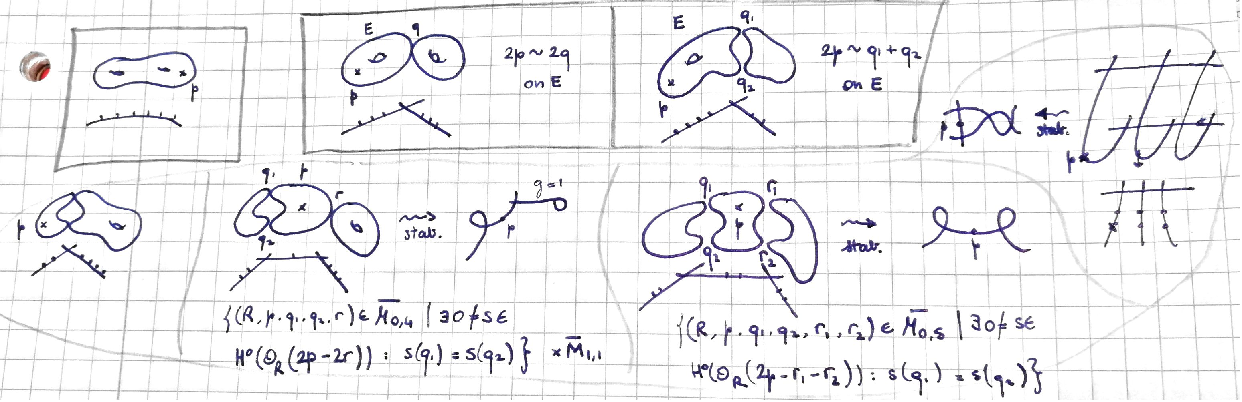
\includegraphics[width=\textwidth]{admissible_Weierstrass}
  \caption{Admissible covers and Weierstrass points.}\label{fig:adm_W}
  \end{figure}
  \end{center}
 \item If $x_1$ and $x_2$ are conjugate, they have to map to the same component of the target of the admissible cover. We may adapt the description of the previous point by replacing every condition on $2x$ by its analogue for $x_1+x_2$.  There are a few more situations to take into account: $x_1$ and $x_2$ could belong to a rational component $R$ bubbling off from a Weierstrass point of a genus two curve; or bridging between two distinct curves of genus one; or $x_1$ and $x_2$ could lie on two distinct rational components $R_1$ and $R_2$ intersecting each other at one node and meeting a curve of genus one in two distinct points (\dag); or $R_1$ and $R_2$ intersecting each other in three points. See Figure \ref{fig:adm_conj}.
  \begin{figure}[!ht]
 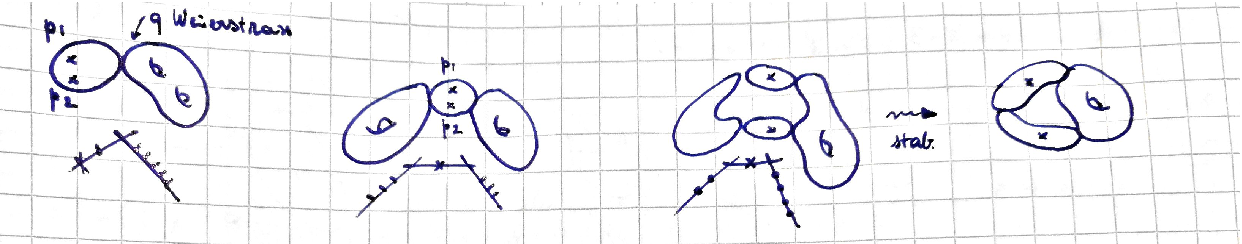
\includegraphics[width=\textwidth]{admissible_conjugate}  
 \caption{Admissible covers and conjugate points.}\label{fig:adm_conj}
  \end{figure}
 \end{itemize}
 
 \begin{rem}\label{rmk:necklace_symmetry}
  In case (\dag), the singularity of the total space of a smoothing $\mathcal C\to\dvr$ at the two distinguished nodes (separating the elliptic component from the rational chain) are both $A_k$ for the same $k$, because they map to the same node of the target in the admissible cover. This consideration is stable under base change, and it therefore entails a symmetry of the rational chain in the model with regular total space.
 \end{rem}
 
 \subsection{Minimal curves}
 \begin{definition}
  A projective Gorenstein curve $C$ is \emph{minimal} if it contains no node $x$ such that the normalisation of $C$ at $x$ consists of two connected components, one of which has genus zero.
 \end{definition}

 When $C$ is nodal, minimal is equivalent to semistable (no rational tails). Compare with \cite[Definition 3.2]{Catanese} for an even stronger notion. When $C$ has arithmetic genus one, this is the same as saying that $C$ contains no separating nodes. Recall \cite[Lemma 3.3]{SMY1}.

\begin{lem}\label{lem:min1}
 A minimal Gorenstein curve $Z$ of arithmetic genus one can be: a smooth elliptic curve; a ring of $r\geq 1$ copies of $\PP^1$; or an elliptic $m$-fold point whose normalisation is the disjoint union of $m$ copies of $\PP^1$. In any case $\omega_Z\simeq\OO_Z$.
\end{lem}

We provide a similar description of minimal curves of genus two; the proof is left to the reader.
\begin{lem}\label{lem:min2}
 A minimal Gorenstein curve of arithmetic genus two can be either:
 \begin{enumerate}
  \item a smooth curve of genus two;
  \item the union of two minimal Gorenstein curves of genus one, $E_1$ and $E_2$, nodally separated by a (possibly empty) rational chain $R$;
  \item the union of a minimal Gorenstein curve of genus one $E$, and a (possibly empty) rational chain $R$, along two distinct nodes;
  \item the union of two copies of $(\PP^1,0,1,\infty)$ with three (possibly empty) rational chains $R_0, R_1, R_\infty$ joining the homonymous points;
  \item\label{case:twice1} an elliptic $m$-fold point whose pointed normalisation is the disjoint union of either $m-2$ copies of $(\PP^1,0)$ and a semistable rational chain $(R,0,\infty)$, or $m-1$ copies of $(\PP^1,0)$ and a $1$-pointed minimal Gorenstein curve of genus one (if the latter is not irreducible and $m\neq 1$, there are two genus one subcurves sharing a rational branch);
  \item\label{case:2} or a singularity of genus two with $m$-branches, whose normalisation is the disjoint union of $m$ copies of $\PP^1$.
 \end{enumerate}

\end{lem}

\begin{rem}\label{rem:special}
In both cases \eqref{case:twice1} and \eqref{case:2} there are \emph{special} branches supporting the degree of $\omega_Z$ (compare with Definition \ref{def:special_branches} and Corollary \ref{cor:deg_dualising}; recall that the restriction of the dualising sheaf to a component introduces a twist by the conductor ideal, see Noether's formula \cite[Proposition 1.2]{Catanese}). Notice that the notion of conjugate points is not always intrinsic to the curve.
\end{rem}

\subsection{Semistable tails}
 Let $\overline{\mathcal C}_0$ be a minimal curve with a genus two singularity of type $I$ (resp. $I\!I$), and let $\overline{\mathcal C}$ be a one-parameter smoothing over a trait $\dvr$. Let $\mathcal P$ denote $\PP(\pi_*\omega_{\overline{\mathcal C}/\dvr})$, which is a $\PP^1$-bundle over $\dvr$. It follows from an easy calculation (or from \cite[Theorem D]{Catanese}) that the canonical series is basepoint-free, and so there is a morphism:
 \bcd
 \overline{\mathcal C}\ar[dr]\ar[rr] & & \mathcal P \ar[dl] \\
 & \dvr &
 \ecd
 such that, in the central fibre, it restricts to a double cover on the special branch (resp. an isomorphism on each of the special branches) and it contracts the axes. The general fibre is the hyperelliptic cover $\overline{\mathcal C}_{\bar\eta}\to\PP^1_{\bar\eta}$, endowing $\PP^1_{\bar\eta}$ with a length $6$ branch divisor $B_{\bar\eta}$. Possibly after passing to a finite cover of $\dvr$, $B_{\bar\eta}$ is actually defined over $\eta$, and we can take the stable model $(\mathcal T,B)$ of $(\PP^1_\eta,B_\eta)$, together with its associated double cover $\mathcal C$. We thus have a diagram:
 \bcd
 \mathcal C\ar[r,"\psi"]\ar[d,"\phi"] & \mathcal T\ar[d]\\
 \overline{\mathcal C} \ar[r] & \mathcal P
 \ecd
 over $\dvr$ (by a slight abuse of notation), where the upper row is a family of admissible covers. 
 
 The line bundle $\OO_{\mathcal P}(1)$ pulls back to $\omega_{\bar \pi}$ on $\overline{\mathcal C}$. Its pullback $\OO_{\mathcal T}(1)$ on $\mathcal T$ has degree $1$ on exactly one component of the tree. Pulling back further to $\mathcal C$, we gather the following information:
 \begin{enumerate}[label=(\alph*)]
  \item $\phi^*\omega_{\bar\pi}=\omega_{\pi}(\pazocal Z)$ for a vertical divisor $\pazocal Z$ supported on the exceptional locus $\operatorname{Exc}(\phi)=: Z$.
  \item $\psi^*\OO_{\mathcal T}(1)=\OO_{\mathcal C}(q+\bar q)$ for a choice of two conjugate points of $\mathcal C$ lying over the same point of $\mathcal T$, belonging to the component on which $\OO_{\mathcal T}(1)$ is ample.
  \item\label{pt:compatibleZ} $\pazocal Z$ is the pullback of a vertical divisor on $\mathcal T$.
 \end{enumerate}
 
 This description leads to the following simple observations:
 
 \begin{enumerate}[label=(\Roman*)]
  \item If $\overline{\mathcal C}_0$ has a type $I$ singularity, the branch of ${\mathcal C}_0$ corresponding to the singular branch of $\overline{\mathcal C}_0$ is attached to a Weierstrass point of $\pazocal Z$ with respect to $\psi$.
  \item If $\overline{\mathcal C}_0$ has a type $I\!I$ singularity, the branches of ${\mathcal C}_0$ corresponding to the twin branches of $\overline{\mathcal C}_0$ are attached to two conjugate points of $\pazocal Z$ with respect to $\psi$.
 \end{enumerate}

 Moreover, the distance of the special branch(es) from the core is always less than that of the axes; the ratio is roughly $1:3$ in case $I$, and $1:2$ in case $I\!I$, but, more precisely, this depends on the relative position of the attaching points of the chains in the dual graph of the core. An elegant treatment uses the language of tropical geometry.

 We consider the tropicalization $\tropC\to\tropT$ of $\psi$ \cite{CMR}. After further base-change and normalised blow-ups, we can assume that $\mathcal C$ has regular total space; this only affects $\tropC$ by subdividing edges, not changing their lengths. Now $\tropC$ is nothing but the dual graph of the special fiber $\mathcal C_0$, with edges of length $1$.
 
 The vertical divisor $\pazocal Z$ can be represented by a piecewise-linear (PL) function on $\tropC$ with integral slope along the edges (see for example \cite{BakerNorine}); moreover, observation \ref{pt:compatibleZ} above shows that $\lambda$ is pulled back from a PL function $\lambda_T$ on $\tropT$ - for this to be true we have to allow half-integral slopes along the edges. Finding $\lambda$ becomes a simple matter of degre-matching on the tree $\tropT$; this shows existence and uniqueness. Recall that the canonical divisor $K_{\tropC}$ has degree:
 \begin{equation}\label{eq:canonical_degree}
 2g(v)-2+\operatorname{val}(v)                                                                                                                                                                                                                                                                                                                                                                                                                                                                                                                                                                                                                                                                                                                                                                                                                                                                                                                                                                                                                                                             \end{equation}
on a vertex $v$ of $\tropC$, where $g\colon V(\tropC)\to\mathbb Z$ is the genus assignment, and $\operatorname{val}(v)$ is the number of bounded edges adjacent to $v$; \eqref{eq:canonical_degree} is also the degree of $\omega_\pi$ when restricted to the component of $\mathcal C_0$ corresponding to $v$.

Notice that $\tropT$ is decorated with six unlabelled legs corresponding to the branch divisor $B$; we call them $B$\emph{-legs}. It follows from the Riemann-Hurwitz formula that the divisor $\OO_{\tropT}(1)$ on $\tropT$ pulling back to $K_{\tropC}$ has degree:
 \[ \operatorname{val}(v^\prime)-2+\frac{1}{2}\#\{f\ B\text{-leg }| f\multimap v^\prime\} \]
 on a vertex $v^\prime$ of $\tropT$. Therefore, the equation that we have to solve is:
 \begin{equation}\label{eqn:Dv}
  \operatorname{val}(v^\prime)-2+\frac{1}{2}\#\{f\ B\text{-leg }| f\multimap v^\prime\}+\sum_{e\multimap v^\prime}s(\overline\lambda_T,e)=1
 \end{equation}
 on the vertex of $\tropT$ corresponding to the special branch, and $0$ otherwise; where $s(\overline\lambda_T,e)$ denotes the outgoing slope of $\overline\lambda_T$ along the edge $e$.

 
  For the reader's benefit, we include Figure \ref{fig:adm_fun_smooth_core} to illustrate the shape of $\lambda$ in the simplest possible case, namely when the core is smooth. The blue numbers represent the slope of $\lambda$ along the corresponding edges. Figure \ref{fig:adm_fun_reducible_core} exhibits how the distance of the axes from the core can vary when the latter becomes more degenerate.
 
 \begin{center}
  \begin{figure}[htb]
  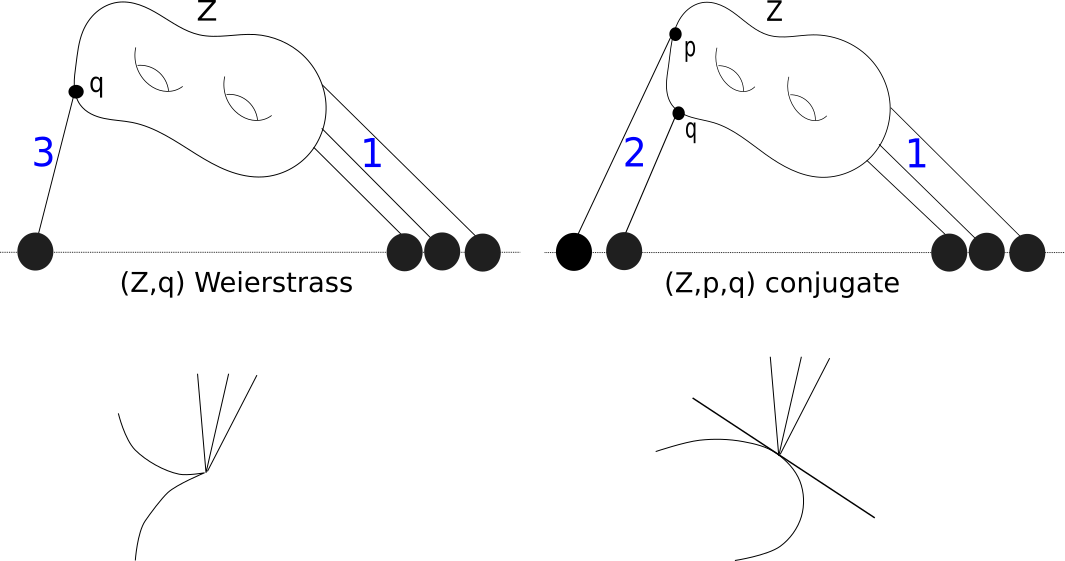
\includegraphics[width=\textwidth]{irreducible_core}
  \caption{Semistable tail of a type $I_4$ (left), resp. type $I\!I_5$ (right), singularity, generic case: the core is smooth, the singular branch is attached to a Weierstrass point (resp. the twin branches are attached to conjugate points), the other branches are attached to distinct points, and the corresponding edge-length is three (resp. two) times longer han the special one.}
  \label{fig:adm_fun_smooth_core}
 \end{figure}
 \end{center}
 
  \begin{center}
  \begin{figure}[h]
  \includegraphics[width=\textwidth]{reducible_core}
  \caption{A more degenerate semistable tail of a type $I_4$ singularity. Here $Z$ consists of $R$, $E$, and $F$ together. $(Z,q)$ is Weierstrass in the sense that $2q\sim 2r\in\operatorname{Pic}(E)$.}
  \label{fig:adm_fun_reducible_core}
 \end{figure}
 \end{center}

 Two important observations allow us to write down $\lambda$ explicitly in all possible situations:
 \begin{enumerate}
  \item The balancing equation \eqref{eqn:Dv} is unaffected by \emph{tropical modifications}, i.e. growing a tree on which $\lambda$ has constant slope $1$.
  \item The balancing equation \eqref{eqn:Dv} is stable under edge contraction.
 \end{enumerate}
 It follows that it is enough to study the case that the core consists of a configuration of rational curves; there are only two stable such configurations, named \emph{dumbbell} and \emph{theta}. Figure \ref{fig:admredcores} (from \cite{BC}) illustrates the situation: we draw both the source (above) and the target (below) of the tropical admissible cover; the blue numbers on the latter represent the slope of $\lambda_T$ - that of $\lambda$ can be recovered by multiplying with the expansion factor of $\psi$; and the red verteices correspond to the special branches. The vertices corresponding to the axes of the genus two singularity do not appear in the picture: they lie at the same height as the red vertices, on an arbitrary configuration of trees emanating from the core, along which $\lambda$ has slope $1$.

\begin{figure}
	\centering
	%\begin{minipage}[t]{0.5\textwidth}
		%\centering
		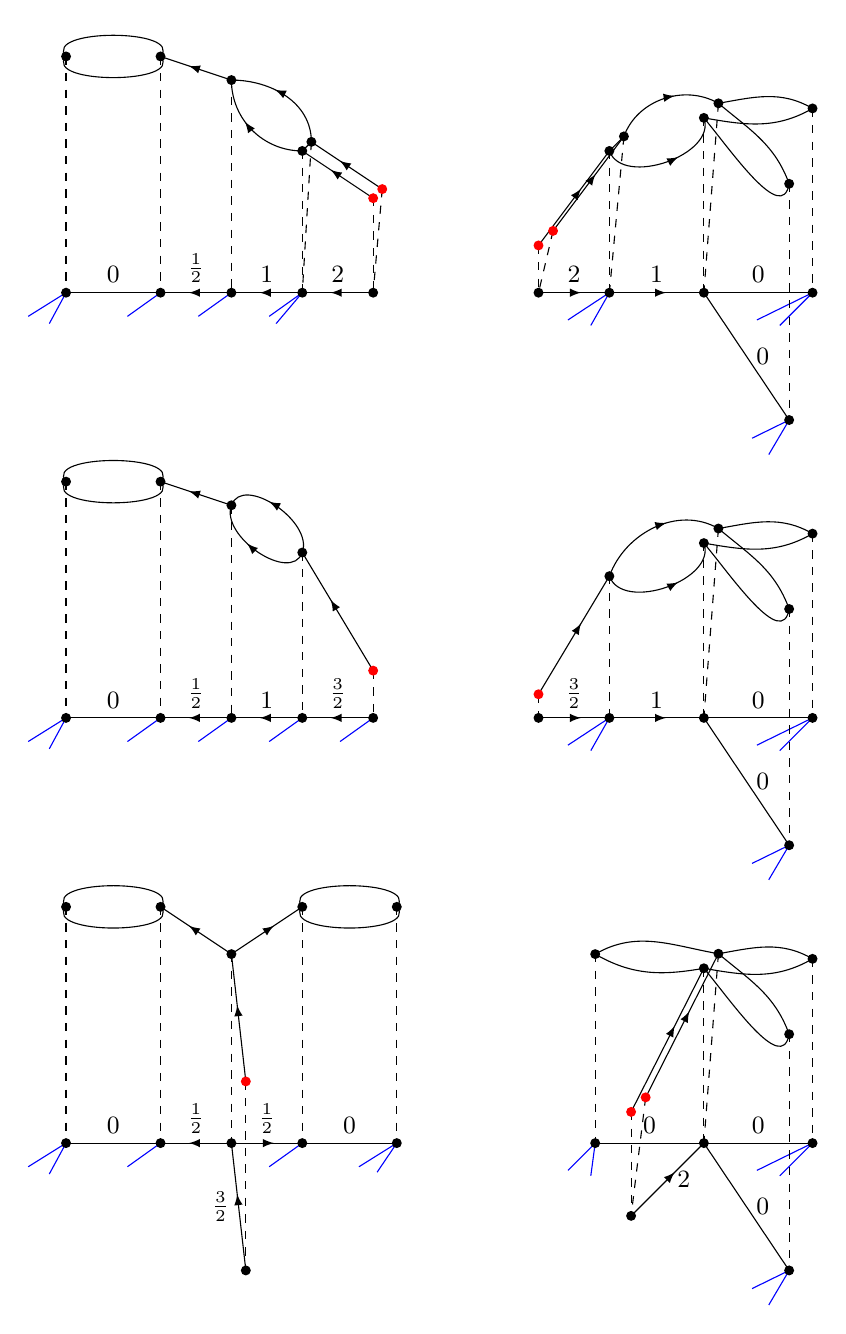
\begin{tikzpicture} [scale=.6]
		\tikzstyle{every node}=[font=\normalsize]
		\tikzset{arrow/.style={latex-latex}}
		\def\S{2.825cm} % Seitenlaenge des Quadrats 



		%coordinates source
		
		\coordinate (A) at (0,6,0);
		  \coordinate (B) at (2,6,0);
		 \coordinate (C) at (3.5,5.5,0);
		 
		  \coordinate (CM) at (3.5,5,0);;%need for case 5
		 	\coordinate (AM) at (5,6,0);%need for case 5
		  \coordinate (BM) at (7,6,0);;%need for case 5
		
		 
		 \coordinate (D) at  (5,4.5,0); 
		 \coordinate (Dd) at (5.5,5.5,0); %need for case 4
		\coordinate (D1) at  (5,4,-.5);%need for case 3
		\coordinate (D2) at  (5,4,0);%need for case 3
		
		\coordinate (Ew) at (6.5,5,7);
		\coordinate (Ee) at (6.5,3.8,0);%need for case 3
		\coordinate (E) at (6.5,2,0); 
         \coordinate (E1) at (6.5,3,-.5); %need for NW
         \coordinate (E2) at ( 6.5,3,0); %need for NW
      %coordinate target
      	\coordinate (At) at (0,1,0);
		  \coordinate (Bt) at (2,1,0);
		 \coordinate (Ct) at (3.5,1,0);
		\coordinate (Dt) at  (5,1,0);
		\coordinate (Et) at (6.5,1,0); 
		\coordinate (Ddt) at (5.5,1,0); %need for 4
		\coordinate (Ewt) at (6.5,1,7);); %need for case 4
		\coordinate (BMt) at (7,1,0);;%need for case 5
      %coordinate markings
      
      
      	
		\coordinate (P1) at (-.3,1,1.3);
		\coordinate (P2) at (.3,1,1.7);
		\coordinate (P3) at (1.8,1,1.3);
		\coordinate (P4) at (3.3,1,1.3);
		\coordinate (P5) at (4.8,1,1.3);
		\coordinate (P6) at (6.3,1,1.3);
		\coordinate (Pp6) at (6.8,1,1.7); %need in 3
		\coordinate (Q6) at (5.1,1,1.7); %need later
        \coordinate (T6) at (6.5,1,6);
        
        \coordinate (QM6) at (6.7,1,1.3); %need in 5
        \coordinate (TM6) at (7.2,1,1.6); %need in 5
      %%%%%%%%%%%%%%%%%%%%%%%%%%%%%%%%%%%%%%%%%%%%
      
      %dumbbell 2
      
      % arrow source
      \draw (A) to [out=130,in=50] (B);
      \draw (A) to [out=-130,in=-50] (B);
      \draw[->-] (C)--(B);
      \draw[->-] (D) to [out=70,in=70](C);
      \draw[->-] (D) to [out=-110,in=-110](C);
       \draw[->-] (E)--(D);
         
        %arrow target
        \draw[->-] (Et)--(Dt);
        \draw[->-] (Dt)--(Ct);
        \draw[->-] (Ct)--(Bt);
        \draw (Bt)--(At);
                

        % Branch points
		\draw[blue] (At)--(P1);
		\draw[blue] (At)--(P2);
		\draw[blue] (Bt)--(P3);
		\draw[blue] (Ct)--(P4);
		\draw[blue] (Dt)--(P5);
		\draw[blue] (Et)--(P6);
		
		%slopes
\node at (1,1,0) [above] {\small{0}};
\node at (2.75,1,0) [above] {\small{$\frac{1}{2}$}};
\node at (4.25,1,0) [above] {\small{$1$}};
\node at (5.75,1,0) [above] {\small{$\frac{3}{2}$}};

       %admissible cover
       
       \draw[dashed] (A)--(At);
        \draw[dashed] (B)--(Bt);
       \draw[dashed] (C)--(Ct);
       \draw[dashed] (D)--(Dt);
        \draw[dashed] (E)--(Et);


      
      \foreach \x in {A,B,C,D,At,Bt,Ct,Dt,Et}
   \fill (\x) circle (3pt);
     	\fill[red] (E) circle (3pt);
     	
%%%%%%%%%%%%%%%%%%%%%%%%%%%%%%%%%%%%%%%%%%%%%%%%%%%%%%

%dumbbell 1

\begin{scope}[every coordinate/.style={shift={(0,9,0)}}]

% arrow source
       \draw ([c]A) to [out=130,in=50] ([c]B);
      \draw ([c]A) to [out=-130,in=-50] ([c]B);
       \draw[->-] ([c]C)--([c]B);
      \draw[->-] ([c]D1) to [out=90,in=0]([c]C);
      \draw[->-] ([c]D2) to [out=-180,in=-90]([c]C);
       \draw[->-] ([c]E1)--([c]D1);
       \draw[->-] ([c]E2)--([c]D2);
       \draw ([c]D1) -- ([c]D2);
         
        %arrow target
        \draw[->-] ([c]Et)--node[above] {\small{$2$}}([c]Dt);
        \draw[->-] ([c]Dt)--node[above] {\small{$1$}}([c]Ct);
        \draw[->-] ([c]Ct)--node[above] {\small{$\frac{1}{2}$}}([c]Bt);
        \draw ([c]Bt)--node[above] {\small{0}}([c]At);
                

        % Branch points
		\draw[blue] ([c]At)--([c]P1);
		\draw[blue] ([c]At)--([c]P2);
		\draw[blue] ([c]Bt)--([c]P3);
		\draw[blue] ([c]Ct)--([c]P4);
		\draw[blue] ([c]Dt)--([c]P5);
		\draw[blue] ([c]Dt)--([c]Q6);
		

       %admissible cover
       
       \draw[dashed] ([c]A)--([c]At);
        \draw[dashed] ([c]B)--([c]Bt);
       \draw[dashed] ([c]C)--([c]Ct);
       \draw[dashed] ([c]D1)--([c]Dt);
       \draw[dashed] ([c]D2)--([c]Dt);
        \draw[dashed] ([c]E1)--([c]Et);
        \draw[dashed] ([c]E2)--([c]Et);


      
      \foreach \x in {A,B,C,D1,D2,At,Bt,Ct,Dt,Et}
   \fill ([c]\x) circle (3pt);
     	\fill[red] ([c]E1) circle (3pt);
     		\fill[red] ([c]E2) circle (3pt);
\end{scope}


 %%%%%%%%%%%%%%%%%%%%%%%%%%%%%%%%%%%%%%%%%%%%%%%%%%
 
 % dumbbell 3 (last)
 
 \begin{scope}[every coordinate/.style={shift={(0,-9,0)}}]

% arrow source
       \draw ([c]A) to [out=130,in=50] ([c]B);
      \draw ([c]A) to [out=-130,in=-50] ([c]B);
       \draw[->-] ([c]CM)--([c]B);
       \draw[->-] ([c]Ew)--([c]CM);
        \draw[->-] ([c]CM)--([c]AM);
      \draw ([c]AM) to [out=130,in=50] ([c]BM);
      \draw ([c]AM) to [out=-130,in=-50] ([c]BM);
      
      %arrow target
        \draw ([c]At)--node[above] {\small{$0$}}([c]Bt);
        \draw[->-] ([c]Ct)--node[above] {\small{$\frac{1}{2}$}}([c]Dt);
        \draw[->-] ([c]Ewt)--node[left]{\small$\frac{3}{2}$}([c]Ct);
        \draw[->-] ([c]Ct)--node[above] {\small{$\frac{1}{2}$}}([c]Bt);
        \draw ([c]Dt)--node[above] {\small{$0$}}([c]BMt);
        
        	
         % Branch points
		\draw[blue] ([c]At)--([c]P1);
		\draw[blue] ([c]At)--([c]P2);
		\draw[blue] ([c]Bt)--([c]P3);
		\draw[blue] ([c]Dt)--([c]P5);
		\draw[blue] ([c]BMt)--([c]QM6);
		\draw[blue] ([c]BMt)--([c]TM6);
		
  
      %admissible cover
       
       \draw[dashed] ([c]A)--([c]At);
        \draw[dashed] ([c]B)--([c]Bt);
       \draw[dashed] ([c]CM)--([c]Ct);
       \draw[dashed] ([c]Ew)--([c]Ewt);
       \draw[dashed] ([c]AM)--([c]Dt);
     \draw[dashed] ([c]BM)--([c]BMt);
     
           
        \foreach \x in {A,B,AM,BM,At,Bt,Ct,Dt,BMt,CM,Ewt}
   \fill ([c]\x) circle (3pt);
     	\fill[red] ([c]Ew) circle (3pt);
                
     

    \end{scope}







%%%%%%%%%%%%%%%%%%%%%%%%%%%%%%%%%%%%%%%%%%%%%%%%%%%%%%

%%%%%%%%%%%%%%%%%%%%%%%%%%%%%%%%%%%%%%%%%%%%%%%%%%

%Theta graph case
\coordinate (Cc) at (0,0.5,0); %need for Weierstrass
\coordinate (C1) at (0,1,0);
\coordinate (C1b) at (0,1,-.8);
\coordinate (A1) at (1.5,3,0);
\coordinate (A1b) at (1.5,3,-.8);

%3rd theta type
\coordinate (G) at (0.2,2.75,0);
\coordinate (F1) at (2,3,0);
\coordinate(F2) at (2,2.5,0);
% 4th Theta Graph 
\coordinate (A14) at (1.2,4,0);
\coordinate (H1) at (3.5,2.2,3.2);
\coordinate (H2) at (3.5,2.2,4);

\coordinate (B1) at (3.5,3.7,-.8);
\coordinate (B2) at (3.5,3.7,0);
\coordinate (A2) at (8,5,7);
\coordinate (A3) at (5.8,3.9,0);

%target

\coordinate (C1t) at (0,0,0);
%target %3rd theta type
\coordinate (Gt) at (0.2,0,0);
\coordinate (Ft) at (2,0,0);

%target 4th theta type

\coordinate (A14t) at (1.2,0,0);
\coordinate (H1t) at (3.5,0,4);


\coordinate (A1t) at (1.5,0,0);
\coordinate (B1t) at (3.5,0,0);
\coordinate (A2t) at (8,0,7);
\coordinate (A3t) at (5.8,0,0); 

%branch points
\coordinate (Q1) at ( 1.2,0,1.5);
\coordinate (Q2) at ( 1.8,0,1.8);
\coordinate (Q3) at ( 8.3,0,8.9);
\coordinate (Q4) at (7.6,0,8);
\coordinate (Q5) at ( 5.2,0,1.5);
\coordinate (Q61) at ( 5.8,0,1.8);




\begin{scope}[every coordinate/.style={shift={(10,10,0)}}]

%%%%% theta 1

\draw[->-] ([c]C1b)--([c]A1b);
\draw[->-] ([c]C1)--([c]A1);
\draw ([c]A1) -- ([c]A1b);
\draw[->-] ([c]A1b) to [out=70,in=150] ([c]B1);
\draw[->-] ([c]A1) to [out=-70,in=-70] ([c]B2);
%\draw ([c]B1)--([c]A3M1);
%\draw ([c]B2)--([c]A3);
\draw ([c]B1) to [out=10,in=150] ([c]A3);
\draw ([c]B2) to [out=-10,in=-150] ([c]A3);
%\draw ([c]B1)--([c]A2b);
\draw ([c]B1) to [out=-40,in=110] ([c]A2);
\draw ([c]B2) to [out=-50,in=-100] ([c]A2);
%%%%%%%%%%%%%%%%%%%%%
     		%target
\draw[->-] ([c]C1t)--node[above] {\small{$2$}}([c]A1t);
\draw[->-] ([c]A1t)--node[above] {\small{$1$}}([c]B1t);
\draw ([c]B1t)--node[right] {\small{$0$}}([c]A2t);
\draw ([c]B1t)--node[above] {\small{$0$}}([c]A3t);

%branched points

		\draw[blue] ([c]A1t)--([c]Q1);
		\draw[blue] ([c]A1t)--([c]Q2);
		\draw[blue] ([c]A2t)--([c]Q3);
		\draw[blue] ([c]A2t)--([c]Q4);
		\draw[blue] ([c]A3t)--([c]Q5);
		\draw[blue] ([c]A3t)--([c]Q61);


 %admissible cover
       
       \draw[dashed] ([c]C1)--([c]C1t);
        \draw[dashed] ([c]C1b)--([c]C1t);
       \draw[dashed] ([c]A1)--([c]A1t);
       \draw[dashed] ([c]A1b)--([c]A1t);
       \draw[dashed] ([c]B1)--([c]B1t);
        \draw[dashed] ([c]B2)--([c]B1t);
        \draw[dashed] ([c]A2)--([c]A2t);
        \draw[dashed] ([c]A3)--([c]A3t);

        
\foreach \x in {A1,A1b,A2,A3,B1,B2,C1t,A1t,B1t,A2t,A3t}
   \fill ([c]\x) circle (3pt);

  \fill[red] ([c]C1) circle (3pt);
    \fill[red] ([c]C1b) circle (3pt);
     		

\end{scope}


\begin{scope}[every coordinate/.style={shift={(10,1,0)}}]

%%%%% theta 2

%\draw[->-] ([c]C1)--([c]A1);
\draw[->-] ([c]Cc)--([c]A1);
\draw[->-] ([c]A1) to [out=70,in=150] ([c]B1);
\draw[->-] ([c]A1) to [out=-70,in=-70] ([c]B2);

\draw ([c]B1) to [out=10,in=150] ([c]A3);
\draw ([c]B2) to [out=-10,in=-150] ([c]A3);
%\draw ([c]B1)--([c]A2b);
\draw ([c]B1) to [out=-40,in=110] ([c]A2);
\draw ([c]B2) to [out=-50,in=-100] ([c]A2);
%\draw ([c]B1)--([c]A3M1);
%\draw ([c]B2)--([c]A3);
%\draw ([c]B1) to [out=10,in=75] ([c]A3);
%\draw ([c]B2) to [out=-10,in=-75] ([c]A3);
%\draw ([c]B1)--([c]A2b);
%\draw ([c]A2b) to [out=55,in=120] ([c]A2);
%\draw ([c]B2) to [out=-100,in=-80] ([c]A2);
%%%%%%%%%%%%%%%%%%%%%
     		%target
\draw[->-] ([c]C1t)--node[above] {\small{$\frac{3}{2}$}}([c]A1t);
\draw[->-] ([c]A1t)--node[above] {\small{$1$}}([c]B1t);
\draw ([c]B1t)--node[right] {\small{$0$}}([c]A2t);
\draw ([c]B1t)--node[above] {\small{$0$}}([c]A3t);

     		
%branched points

		\draw[blue] ([c]A1t)--([c]Q1);
		\draw[blue] ([c]A1t)--([c]Q2);
		\draw[blue] ([c]A2t)--([c]Q3);
		\draw[blue] ([c]A2t)--([c]Q4);
		\draw[blue] ([c]A3t)--([c]Q5);
		\draw[blue] ([c]A3t)--([c]Q61);

\foreach \x in {A1,A2,A3,B1,B2,C1t,A1t,B1t,A2t,A3t}
   \fill ([c]\x) circle (3pt);
  
     		%\fill[red] ([c]C2) circle (3pt);
     	


 %admissible cover
       
       \draw[dashed] ([c]Cc)--([c]C1t);
        %\draw[dashed] ([c]C2)--([c]C1t);
       \draw[dashed] ([c]A1)--([c]A1t);
       \draw[dashed] ([c]B1)--([c]B1t);
        \draw[dashed] ([c]B2)--([c]B1t);
        \draw[dashed] ([c]A2)--([c]A2t);
        \draw[dashed] ([c]A3)--([c]A3t);
        
         \fill[red] ([c]Cc) circle (3pt);
\end{scope}







\begin{scope}[every coordinate/.style={shift={(10,-8,0)}}]

%%%% theta 3 (last)

\draw ([c]B1) to [out=170,in=30] ([c]A14);
\draw ([c]B2) to [out=190,in=-30] ([c]A14);

\draw[->-] ([c]H1) to ([c]B1);
\draw[->-] ([c]H2) to ([c]B2);
\draw ([c]B1) to [out=10,in=150] ([c]A3);
\draw ([c]B2) to [out=-10,in=-150] ([c]A3);

\draw ([c]B1) to [out=-40,in=110] ([c]A2);
\draw ([c]B2) to [out=-50,in=-100] ([c]A2);

%%%%%%%%%%%%%%%%%%%%%
     		%target
\draw ([c]A14t)--node[above] {\small{$0$}}([c]B1t);
\draw[->-] ([c]H1t)--node[right] {\small{$2$}}([c]B1t);
\draw ([c]B1t)--node[right] {\small{$0$}}([c]A2t);
\draw ([c]B1t)--node[above] {\small{$0$}}([c]A3t);

%branched points

		\draw[blue] ([c]A14t)--([c]Q1);
		\draw[blue] ([c]A14t)--([c]Q2);
		\draw[blue] ([c]A2t)--([c]Q3);
		\draw[blue] ([c]A2t)--([c]Q4);
		\draw[blue] ([c]A3t)--([c]Q5);
		\draw[blue] ([c]A3t)--([c]Q61);

\foreach \x in {A14,A2,A3,B1,B2,H1t, A14t,B1t,A2t,A3t}
   \fill ([c]\x) circle (3pt);
  
     		%\fill[red] ([c]C2) circle (3pt);
     		
     		
     		


 %admissible cover
       
       \draw[dashed] ([c]A14)--([c]A14t);
        %\draw[dashed] ([c]C2)--([c]C1t);
       \draw[dashed] ([c]H1)--([c]H1t);
       \draw[dashed] ([c]H2)--([c]H1t);
     \draw[dashed] ([c]B1)--([c]B1t);
        \draw[dashed] ([c]B2)--([c]B1t);
        \draw[dashed] ([c]A2)--([c]A2t);
        \draw[dashed] ([c]A3)--([c]A3t);
        
 \fill[red] ([c]H1) circle (3pt);
   \fill[red] ([c]H2) circle (3pt);
\end{scope}
\end{tikzpicture}
	%\end{minipage}
\caption{Tropicalization of semistable tails with maximally degenerated core: the dumbbell (l), and the theta graph (r). The red vertices correspond to the special branches.}
\label{fig:admredcores}
\end{figure}
%\clearpage
 
 Summing up, we have proven the following:

\begin{prop}\label{prop:tailI}
 Let $\phi\colon\mathcal C\to\overline{\mathcal C}$ be a birational contraction over the spectrum of a discrete valuation ring $\dvr$, where: $\mathcal C\to \dvr$ is a family of prestable (reduced, nodal) curves of arithmetic genus two with smooth generic fibre $\mathcal C_{\eta}$; $\overline{\mathcal C}\to\dvr$ is a family of Gorenstein curves with a genus two singularity of type $I_m$ (resp. $I\!I_m$) at $q\in\overline{\mathcal C}_0$. Denote by $(Z;q_1,\ldots,q_m)$ the exceptional locus $\Exc(\phi)=\phi^{-1}(q)$, marked with $Z\cap\overline{\mathcal C_0\setminus Z}$, where $q_m$ corresponds to the singular branch of $\overline{\mathcal C}_0$ (resp. $q_1,q_m$ correspond to the twin branches of $\overline{\mathcal C}_0$). Then:
 \begin{enumerate}[leftmargin=.6cm]
  \item $(Z,q_m)$ is Weierstrass (resp. $(Z,q_1,q_m)$ is conjugate).
  \item On $\operatorname{trop}(\mathcal C)$, the distance of $q_m$ (resp. $q_1$ and $q_m$ - they are equidistant) from the core is less than the distance of any other $q_i$ from the core, and the former - together with the shape of $\operatorname{trop}(Z)$ - determines the latter.
 \end{enumerate}
\end{prop}

Viceversa, every such genus two subcurve can be contracted to a Gorenstein singularity.

\begin{prop}\label{prop:contractionI}
 Let $(\mathcal C,p_1,\ldots,p_n)\to\dvr$ be a family of pointed semistable curves of arithmetic genus two such that $\mathcal C$ has regular total space and smooth generic fibre, and $(\mathcal C,p_1)\to \Delta$ is Weierstrass (resp. $(\mathcal C,p_1,\bar p_1)\to \Delta$ is conjugate). Let $(Z,q_1,\ldots,q_m)$ be a genus two subcurve of $\mathcal C_0$ containing none of the $p_i(0)$, marked by $Z\cap \overline{\mathcal C_0\setminus Z}$ so that the tail containing $p_1$ is attached to $Z$ at $q_m$ (resp. the tails containing $p_1$ and $\bar p_1$ are attached to $Z$ at $q_1$ and $q_m$), and satisfying all the shape prescriptions above. There exists a contraction $\phi\colon\mathcal C\to\overline{\mathcal C}$ over $\dvr$, with exceptional locus $Z$, such that $\overline{\mathcal C}\to\dvr$ is a family of Gorenstein curves containing a type $I_m$ (resp. type $I\!I_m$) singularity in the central fibre.
\end{prop}

\begin{comment}

\begin{proof}(of Proposition \ref{prop:tailI}) By blowing down all the rational trees on $\overline{\mathcal C}_0$, we can assume that the latter does not contain any separating node. Consider then the hyperelliptic cover $\tau\colon\overline{\mathcal C}\to\PP(\bar\pi_*\omega_{\overline{\mathcal C}/\dvr})$; restricting to the central fibre, $\tau$ contracts all axes, and induces a two-fold cover of $\PP^1$ by the special branch, ramified at the singularity and at another point; in fact, we can extend the image of this point to a section of $\PP(\bar\pi_*\omega_{\overline{\mathcal C}/\dvr})$ lying inside the branch locus of $\tau$. By pulling this back to $\mathcal C$ via $\tau\circ\phi$ we get a horizontal divisor $\Delta^\prime$; clearly, the stable model of $(\mathcal C,\Delta^\prime)$ is Weierstrass, and its central fibre coincides with the stabilisation of $(Z,q_m)$. This proves the first claim. (The proof of Proposition \ref{prop:tailII}(1) is entirely analogous, by noticing that the preimage of a generic hyperplane section of $\PP(\bar\pi_*\omega_{\overline{\mathcal C}/\dvr})$ will mark the two special branches of $\overline{\mathcal C}_0$.)

We now come to a proof of the more combinatorial claim (2) of the Proposition. Since $\overline{\mathcal C}\to \Delta$ is Gorenstein, and $\phi$ is assumed to be an isomorphism outside $Z$, because the dualising sheaf behaves well under restriction to open subschemes, we have an equality of line bundles:
\[ \phi^*\omega_{\overline{\mathcal C}/\dvr}=\omega_{\mathcal C/\dvr}(D),\]
for some effective (Cartier) divisor $D$ on $\mathcal C$ supported on $Z$. The next lemma will help us determine the coefficients of $D$ along the components of $Z$ containing $q_i$.

\begin{lem}\label{lem:dualising_lb}
 Let $\nu\colon C\to \bar C$ be the normalisation of a Gorenstein singularity of genus two, with $\nu^{-1}(q)=\{q_1,\ldots,q_m\}$. Then  $\nu^*\omega_{\bar C}=\omega_C(2q_1+\ldots+2q_{m-1}+4q_m)$ (type $I$) or $\nu^*\omega_{\bar C}=\omega_C(3q_1+2q_2+\ldots+2q_{m-1}+3q_m)$ (type $I\!I$).
\end{lem}
\begin{proof}
 The dualising sheaf of a reduced curve admits an explicit description (due to Rosenlicht, see e.g. \cite[Proposition VIII.1.16]{AK}) in terms of residues:
 \[\omega_{\bar C}(U)=\{\eta\in \Omega_{C}\otimes K(\nu^{-1}(U)) | \sum_{p_i\in\nu^{-1}(p),p\in U}\operatorname{Res}_{p_i}((\nu^*f)\eta)=0,\ \forall f\in\OO_{\bar C}(U)\}.\]
 We are going to use the explicit coordinates in \eqref{coordII-cs} and \eqref{coordIII-cs}.
 In case $I$, we know that $\tm^4\subseteq R$, therefore we have poles of fourth order at most. It is enough to study the possible polar tails. On the other hand, $t_i^2\in R$ for all $i$ implies the part of order three is trivial. So let \[\eta=c_1\frac{\operatorname{d}t_1}{t_1^4}+b_1\frac{\operatorname{d}t_1}{t_1^2}+a_1\frac{\operatorname{d}t_1}{t_1}\oplus\ldots\oplus c_m\frac{\operatorname{d}t_m}{t_m^4}+b_m\frac{\operatorname{d}t_m}{t_m^2}+a_m\frac{\operatorname{d}t_m}{t_m}.\]
 From looking at $1\cdot\eta$ we deduce $\sum_{i=1}^m a_i=0$; from $x_i\cdot\eta$ we see $b_i+c_m=0$ for all $i$, and from $x_i^3\cdot\eta$ we have $c_i=0$ for all $i$. (The statement about third order poles can be evinced from $x_i^2\cdot\eta$ or from $z\cdot\eta$ indifferently.) Therefore $\omega_C/\nu_*\omega_{\tilde C}$ is spanned by
 \begin{align*}
  \frac{\operatorname{d}t_1}{t_1}-\frac{\operatorname{d}t_m}{t_m},\ldots,\frac{\operatorname{d}t_{m-1}}{t_{m-1}}-\frac{\operatorname{d}t_m}{t_m},\frac{\operatorname{d}t_m}{t_m^2}\\
  \bar{\eta}=\frac{\operatorname{d}t_1}{t_1^2}+\ldots+\frac{\operatorname{d}t_{m-1}}{t_{m-1}^2}-\frac{\operatorname{d}t_m}{t_m^4}.
 \end{align*}
In particular $\omega_C$ is generated by $\bar{\eta}$ as an $\OO_C$-module. 

In case $I\!I$, we know that $\tm^3\subseteq R$, so we have poles of third order at most. Let \[\eta=c_1\frac{\operatorname{d}t_1}{t_1^3}+b_1\frac{\operatorname{d}t_1}{t_1^2}+a_1\frac{\operatorname{d}t_1}{t_1}\oplus\ldots\oplus c_m\frac{\operatorname{d}t_m}{t_m^3}+b_m\frac{\operatorname{d}t_m}{t_m^2}+a_m\frac{\operatorname{d}t_m}{t_m}.\]
 From looking at $1\cdot\eta$ we deduce $\sum_{i=1}^m a_i=0$; from $x_i\cdot\eta$ we see $b_1+b_m=0$ (if $i=1$), and $b_i+c_m=0$ (if $i=2,\ldots,m-1$); finally from $x_i^2\cdot\eta$ we have $c_1+c_m=0$ (if $i=1$), and $c_i=0$ (if $i=2,\ldots,m-1$). Therefore $\omega_C/\nu_*\omega_{\tilde C}$ is spanned by
 \begin{align*}
  \frac{\operatorname{d}t_1}{t_1}-\frac{\operatorname{d}t_m}{t_m},\ldots,\frac{\operatorname{d}t_{m-1}}{t_{m-1}}-\frac{\operatorname{d}t_m}{t_m},\frac{\operatorname{d}t_1}{t_1^2}-\frac{\operatorname{d}t_m}{t_m^2},\\
  \bar{\eta}=\frac{\operatorname{d}t_1}{t_1^3}+\frac{\operatorname{d}t_2}{t_2^2}+\ldots+\frac{\operatorname{d}t_{m-1}}{t_{m-1}^2}-\frac{\operatorname{d}t_m}{t_m^3}.
 \end{align*}
In particular $\omega_C$ is generated by $\bar{\eta}$ as an $\OO_C$-module.

\end{proof}

\begin{cor}\label{cor:deg_dualising}
 The multi-degree of $\omega_C$ is $(0,\ldots,0,2)$ in case $I$, and $(1,0,\ldots,0,1)$ in case $I\!I$.
\end{cor}

\begin{rem}
 It follows from this and Corollary \ref{cor:explicitnoaut} that the finiteness of automorphism groups, $H^0(\bar C,\Omega_{\bar C}^\vee(-\sum_{i=1}^np_i))=0$, implies $\omega_{\bar C}(\sum_{i=1}^np_i)$ is ample.
\end{rem}
Let us go back to the proof of Proposition \ref{prop:tailI}. Note that $\phi_{|\mathcal C_0\setminus Z}$ is the normalisation of $\overline{\mathcal C}_0$ at $q$. Letting $T_i$ be the tail of $\mathcal C_0\setminus Z$ attached to $Z$ at $q_i$, by the adjunction formula $\omega_{\mathcal C/\dvr|T_i}=\omega_{T_i}(q_i)$; it follows from Lemma \ref{lem:dualising_lb} that $D$ has multiplicity $3$ at the component of $Z$ containing $q_m$ (case $I$) - resp. $2$ at the components containing $q_1$ and $q_m$ (case $I\!I$) -, and $1$ at any other component containing a $q_i$. Set $\mathcal L=\omega_{\mathcal C/\dvr}(D)=\phi^*\omega_{\overline{\mathcal C}/\dvr}$; we draw the consequences of $\mathcal L_{|Z}=\OO_Z$. We split $Z$ into a core $K$ and a number of rational trees. By Castelnuovo criterion, we may assume that $Z$ is semistable (hence, there are at most $m$ rational trees).

Let $d_A$ denote the multiplicity of the divisor $D$ along the component $A$ of $Z$. First, we claim that no component can appear with $d_A=0$. Assume that this occurred along one of the rational trees. Call $S$ ($S\simeq\PP^1$) a component furthest from the core such that $d_S=0$; $R$ the one that precedes it, and $T_1,\ldots, T_h$ the ones that follow it (when sweeping the tree from the core) - so that $h\geq1$ by the previous paragraph, and $d_{T_i}\geq 1$ by inductive assumption. Then, by adjunction,
 \[\deg(\mathcal L_{|S})= -2+(h+1)+d_R+\sum d_{T_i}=0,\]
 which necessarily implies $h=1$, and $d_R=d_{T_i}=0$, contradicting the assumption. The case that $S$ belongs to the core is similar ($\omega_S$ might only be more positive).
 \begin{center}
 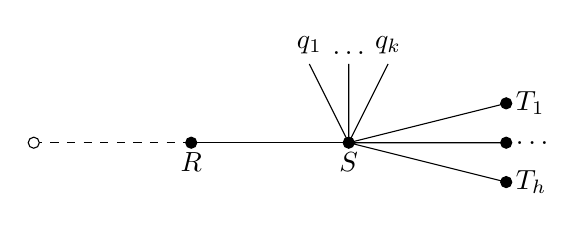
\begin{tikzpicture}
  \draw[dashed] (-2,0) -- (0,0);
  \draw (0,0) node[below]{$R$} --(2,0) node[below]{$S$};
  \draw (2,0) -- (1.5,1) node[above]{$q_1$} (2,0) -- (2,1) node[above]{$\ldots$} (2,0) -- (2.5,1) node[above]{$q_k$};
  \draw (2,0) -- (4,.5) node[right]{$T_1$} (2,0) -- (4,0) node[right]{$\ldots$} (2,0) -- (4,-.5) node[right]{$T_h$};
  \draw[fill=black] (0,0) circle(2pt) (2,0) circle(2pt) (4,.5) circle(2pt) (4,0) circle(2pt) (4,-.5) circle(2pt);
  \draw[fill=white] (-2,0) circle(2pt);
 \end{tikzpicture}
\end{center}
 
Let us now consider $d_S=1$. We stick to the notation above; furthermore, there may be a number $k$ of $q_i$, $i\in\{(1,)2,\ldots,m-1\}$ in case $I\!I$ (resp. $I$), lying on $S$. Then, again by adjunction,
 \[\deg(\mathcal L_{|S})= -2+d_R+\sum d_{T_i}=0.\]
 so either $d_R=2$, $h=0$ and $k\geq 1$ arbitrary, i.e. $S$ is adjacent to $\overline{C\setminus Z}$; or $d_R=1$, $h=1$, and $d_{T_1}=1$ (with $k$ arbitrary). In the latter case, though, by repeating the same argument on $T_1$ etc., we would find an infinite chain in $Z$. 
 \begin{rem}\label{rmk:ignoring_1-trees}
  More generally, an analogous computation shows that, when balancing a component $A$ of multiplicity $d_A$, all neighbouring components of multiplicity $d_A-1$ can be safely ignored.% (at the same time, the number of such components is bounded only by $m$, due to the semistability of $Z$).
 \end{rem}

 We now prove that $d_R>d_S$ holds in general for $S$ on a rational tree. The preceding paragraphs deal with the cases $d_S=0,1$; we may therefore assume $d_S>1$ (which in particular implies $0\leq k\leq 2$). We have
 \[\deg(\mathcal L_{|S})= -2+d_R-(d_S-1)(h+k+1)+\sum d_{T_i}=0.\]
 By proceeding inductively from leaves to root, we can assume that $d_S>d_{T_i},\ i=1,\ldots,h$. We may therefore rewrite the previous equality as
 \[d_R=(d_S-1)(h+k+1)-\sum d_{T_i}+2\geq(d_S-1)(k+1)+2=d_S+1+k(d_S-1)>d_S.\]
 
In fact, we can prove as on \cite[p.893]{SMY1} that $d_R=d_S+1$, unless $d_S=3$ and $q_m\in S$ (type $I$), or $d_S=2$ and either $q_1$ or $q_m$ (or both) are on $S$ (type $I\!I$). We introduce some terminology to describe the weighted dual graph of $D$.

\begin{definition}
 A $t$-chain is a weighted graph that is a chain and such that the weight of two adjacent vertices differ by $t$. We call $t$ the \emph{trend}; the vertex with highest (resp. lowest) weight is called the root (resp. leaf) of the chain. An $(a,t)$-chain is a $t$-chain with leaf weight $a$. The chain $C_1$ can be attached to the chain $C_0$ by identifying the root of $C_1$ with a vertex of $C_0$ having the same weight. A $1$-tree is obtained by attaching a number of $(1,1)$-chains among themselves.
\end{definition}

Let us now look at a component $S$ with $d_S=2$ and at least one of $q_1$ and $q_m$ attached to it (case $I\!I$). The balancing equation is
\[\deg(\mathcal L_{|S})= -2-(h+k+1)+d_R+\sum d_{T_i}=0,\]
with $k\in\{1,2\}$. The preceding discussion implies that $d_{T_i}=1$ for all $i=1,\ldots,h$, so $d_R=3+k$. If $k=2$, i.e. both $q_1$ and $q_m$ are on $S$ - in which case they are indeed equidistant from the core -, then $d_R=5$, and it can be shown inductively that the trend on the chain connecting $S$ to the core is $3$. The same holds in case $I$, with $q_m$ attached to $S$ and $d_S=3$.

Finally, say $d_S=2$ and only $q_1\in S$. Then $d_R=4$, and the trend along the chain that connects $S$ to the core is $2$, unless there is a component $S^\prime$ at which two $2$-chains meet, in which case the trend becomes $3$ after $S^\prime$.

\begin{definition}
 A $2$-tree is obtained by attaching a number of $(1,1)$-chains to a $(2,2)$-chain. A $3$-tree is obtained by attaching a number of $(1,1)$-chains either to a $(3,3)$-chain, or to a weighted graph which is itself obtained by attaching two $(2,2)$-chains to the leaf of a $3$-chain.
\end{definition}

From the preceding discussion, it is clear that the weighted dual graph of $D$ is obtained by attaching a number of $1$-trees, and either (a) one $3$-tree or (b) two $2$-trees to the dual graph of the core $K$, weighted in an appropriate fashion.

Finally, let us look at the core $K$. Consider it as a one-pointed (case (a)), resp. two-pointed (case (b)) curve of genus two, by ignoring all the attachment points of the $1$-trees (it does not alter the balancing equation along $K$ by Remark \ref{rmk:ignoring_1-trees}), and let $\bar K\in\oM_{2,1}$ (resp. $\oM_{2,2}$) be its stable model. The following can happen:

\begin{enumerate}[leftmargin=.6cm]

 \item $K$ is a smooth curve of genus two. In case (a), let $R$ be the component adjacent to the core along the $3$-tree, and let $x=R\cap K$; then $d_K=d_R+3$ by balancing $R$. Balancing $K$ gives \[\omega_{\mathcal C/\dvr}(d_RR+d_KK)_{|K}=\omega_K(d_Rx-(d_R+2)x)\simeq\OO_K,\]
 which admits a solution if and only if $K$ is Weierstrass. Similarly, case (b) can be balanced if and only if $K$ is conjugate.
 
 \item\label{E_E} $K$ contains two distinct subcurves of genus one $E_1$ and $E_2$. We start by solving the balancing equation on one of them, say $E=E_1$.
 If all but one of the neighbouring components have multiplicity $d_E-1$, then the last one is forced to have multiplicity $d_E-1$ as well (by degree reasons). The case that all but two neighbouring components have multiplicity $d_E-1$ occurs when either one $2$-tree or one $3$-tree (and exactly one) is attached to $E$ at $x$; let $F$ be the other component with undetermined multiplicity, which lies between $E_1$ and $E_2$ (possibly $F=E_2$), and let $E\cap F=\{y\}$. The case of a $2$-tree forces $d_F=d_E$ by degree reason, but then we are left to solve $x\sim y$ in $\Pic(E)$, which is impossible; on the other hand, the case of a $3$-tree imposes $d_F=d_E+1$ and $2x\sim 2y$ in $\Pic(E)$, i.e. $K$ is Weierstrass. By the same token, the two $2$-trees have to hit the same genus one curve, say $E_1$, in points $x_1,x_2$ such that $x_1+x_2\sim 2y\in\Pic(E_1)$ and $d_F=d_E+1$.
 
 Assume now there is a chain of rational curves $S_i$ between $E_1$ and $E_2$ in $K$, and one of the special trees cleaves to one of the $S_i$; in case (b), then, both $2$-trees must connect to (possibly different) $S_i$, by the previous paragraph. Moreover, the trend along the rational chains at $E_1$ and $E_2$ has to be $1$. This in turn implies that the trend along the chain separating the two $2$-trees is $0$ (case (b)). In particular, the two $2$-trees are attached to components with the same multiplicity for $D$, so $q_1$ and $q_m$ are equidistant from the core. See the examples in Figure \ref{fig:E1E2}.
 
 %\begin{figure}[h]
 %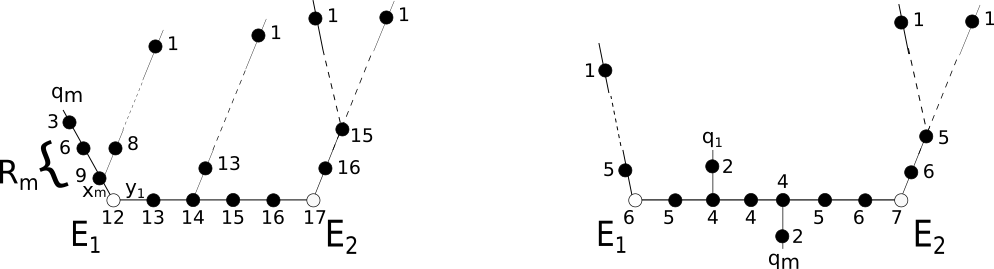
\includegraphics[width=\textwidth]{E1E2example} 
 %\caption{Examples of $Z$ with two genus one components (the white dots). The numbers indicate the multiplicity of $D$. On the left, one $3$-tree attached to $E_1$; on the right, two $2$-trees attached to the rational chain separating $E_1$ from $E_2$.}\label{fig:E1E2}
 % \end{figure}
  
 \item\label{KinDirr} $K$ contains an irreducible subcurve of arithmetic genus one $E$, with two points $y_1$ and $y_2$ on $E$ that are joined in $K$ by a (possibly empty) rational chain. We see as above that either a $3$-tree is attached to a point $x\in E$ satisfying $2x\sim y_1+y_2$ in $\Pic(E)$, or two $2$-trees are attached to $x_1,x_2\in E$ satisfying $x_1+x_2\sim y_1+y_2$ in $\Pic(E)$, or the rational chain is not empty and all the distinguished trees are attached to it. In this case, solve the balancing equation on $E$: let $d=d_E$, $d_1$ and $d_2$ be the multiplicities of the rational components attached to $y_1$ and $y_2$ respectively; then either $d_1=d_2=d-1$, or $d_1=d-1+k$, $d_2=d-1-k$ and $r_1-r_2$ is $k$-torsion in $\Pic(E)$. But, by chasing the balancing equation along the rational necklace, we find that, if $k\geq 1$, then the trend increases when passing through a distinguished bead, so that ultimately $d-1-k=d_2>d_1=d-1+k$, contradiction. So the only possibility is to have a rational chain symmetric with respect to the distinguished beads, namely: in case (a) the two portions of the rational chain lying between the special bead and $E$ have the same length, and in case (b) the distance of the shortest path between a special bead and $E$ is the same for the two special beads. Compare with Remark \ref{rmk:necklace_symmetry} and Figure \ref{fig:ER}.
 
 \begin{figure}
    \centering
    \begin{minipage}[b]{0.48\textwidth}
        \centering
        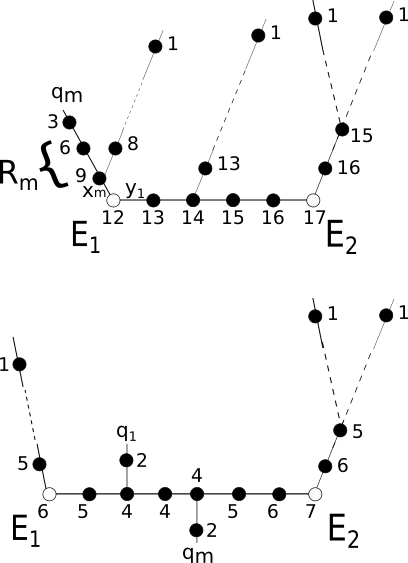
\includegraphics[width=0.7\textwidth]{E1E2example_v} % first figure itself
        \caption{Examples of $Z$ with two genus one components (the white discs). The numbers indicate the multiplicity of $D$. Above, one $3$-tree attached to $E_1$; below, two $2$-trees attached to the rational chain separating $E_1$ from $E_2$.}\label{fig:E1E2}
    \end{minipage}\hfill
    \begin{minipage}[b]{0.48\textwidth}
        \centering
        \includegraphics[width=\textwidth]{ERexample} % second figure itself
        \caption{$K$ is a genus one curve $E$ with a rational bridge $R$. Left column, one $3$-tree; right column, two $2$-trees. Above: the special trees connect to $E$; below: they connect to $R$ - note that $R$ is necessarily symmetric in this case.}\label{fig:ER}
    \end{minipage}
\end{figure}

%  \begin{figure}[hbtp]
% \includegraphics[width=.5\textwidth]{ERexample}
% \caption{$K$ is a genus one curve $E$ with a rational bridge $R$. Left column, one $3$-tree; right column, two $2$-trees. Above: the special trees connect to $E$; below: they connect to $R$ - note that $R$ is necessarily symmetric in this case.}\label{fig:ER}
%  \end{figure}
 
 \item Finally, consider the case of geometric genus $0$. There are two trivalent graphs of genus two.
 \begin{center}
  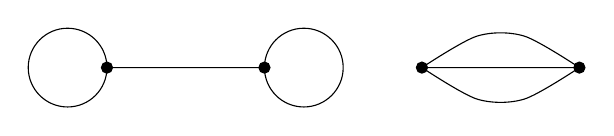
\begin{tikzpicture}
   \draw[fill=black] (-4,0) circle(2pt) -- (-2,0) circle(2pt);
   \draw (-4.5,0) circle(.5) (-1.5,0) circle(.5);
   \draw[fill=black] (0,0) circle(2pt) -- (2,0) circle(2pt); 
   \draw plot [smooth] coordinates {(0,0) (.7,.4) (1.3,.4) (2,0)};
   \draw plot [smooth] coordinates {(0,0) (.7,-.4) (1.3,-.4) (2,0)};
  \end{tikzpicture}
 \end{center}
The graph on the left can be dealt with as a degeneration of cases \eqref{E_E} and \eqref{KinDirr} above; note that if only one of the $2$-trees cleaves to a rational bridge, the balancing equation admits no solution, and, furthermore, if the special trees cleave to a rational loop, then the latter needs to be symmetric (Remark \ref{rmk:necklace_symmetry}).

The graph on the right is the union of two stable components along three semistable chains. It is easy to see that, if a special tree cleaves to a stable component, the only chance that the balancing condition may be satisfied is that there are two $2$-trees and they cleave to different stable components; the semistable chains have arbitrary length and $D$ has the same multiplicity along every component of the core; see the upper left corner of Figure \ref{fig:Krat}. There remain three possibilities for the dual graph, according to how the distinguished components (denoted by $R$) and the other stable components (denoted by $A$ and $B$) distribute themselves.

  \begin{figure}[hbtp]
 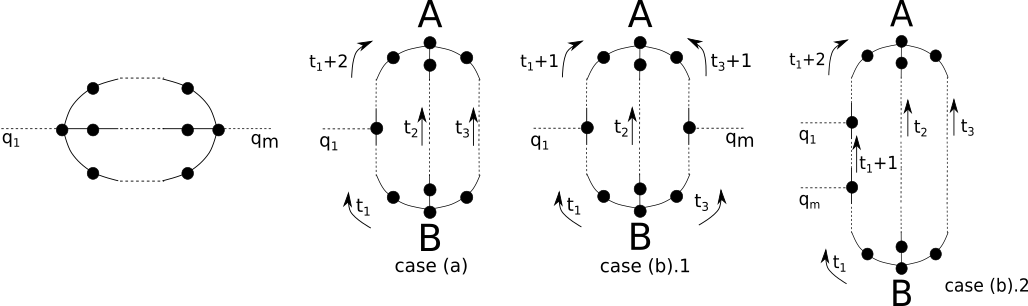
\includegraphics[width=\textwidth]{rational_pretzel_h} 
 \caption{When $K$ consists of rational curves.}\label{fig:Krat}
  \end{figure}
  
 Denoting by $t$ the trend along various rational chains, we find that in case (a) and (b).2 balancing along $A$ or $B$ is equivalent to $\sum_it_i=1$. Assume $t_1\geq0$; then $d_A>d_B$, therefore $t_2,t_3>0$, which contradicts $\sum_it_i=1$. Similarly, if $t_1\leq -2$, then $d_A<d_B$, therefore $t_2,t_3<0$, which makes $\sum_it_i=1$ again impossible. We find only one solution with $t_1=-1$ and $t_2=t_3=0$ - notice that it is a degeneration of case \ref{KinDirr} above.
 In case (b).1, we find $\sum_it_i=1$ when balancing $B$, and $\sum_it_i=-1$ when balancing $A$, which is a contradiction.
\end{enumerate}
This concludes the proof of Propositions \ref{prop:tailI}(2) and \ref{prop:tailII}(2).
\end{proof}
\begin{rem}\label{rmk:extra_conjugate}
When the special trees cleave to a rational component $R$, solving the balancing equation imposes no restriction on the relative position of special points on $R$. In case they do not satisfy the Weierstrass condition (see Section \ref{rmk:Wandconj}), we may still find an effective $D$ such that $\omega_{\mathcal C/\dvr}(D)$ is trivial on $Z$; we wonder whether this line bundle might not be semiample though.
%There is a stable $2$-pointed curve that arises as a solution of the balancing equation, yet is not conjugate, namely:
%  \begin{center}
% 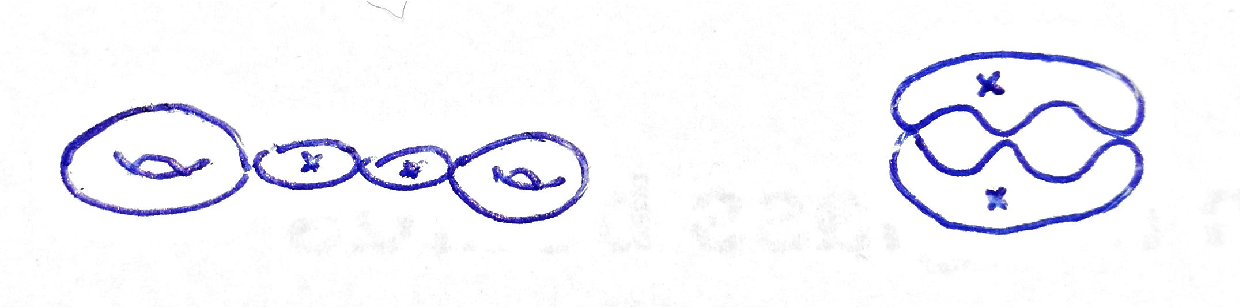
\includegraphics[width=.6\textwidth]{extra_conjugate}  
%  \end{center}
%In this case, the line bundle $\omega_{\mathcal C/\dvr}(D)$ trivial along $Z$ might not be semiample.
\end{rem}

\end{comment}

\begin{proof}(of Proposition \ref{prop:contractionI})
 By blowing down some rational tails outside $Z$, we can assume that $\mathcal C_0\setminus Z=\sqcup_{i=1}^m T_i$ with each $T_i\simeq\PP^1$. The image of $p_i(0)$ and $p_j(0)$ might now coincide for $i\neq j$. The total space of the curve can still be assumed to be smooth by the Castelnuovo criterion. By abuse of notation, we denote the resulting family of pointed curves by $(\mathcal C,p_1,\ldots,p_n)$. By assumption on the shape of $Z$, we can find an effective Cartier $\pazocal Z$ supported on $Z$ such that $\mathcal L=\omega_{\mathcal C/\dvr}(\pazocal Z+\sum p_i)$ is trivial on $Z$ and relatively ample elsewhere (both on $T_i$ and on the generic fibre). Consider a second line bundle $\mathcal L^\prime=\OO(2p_1+\sum p_i)$ (resp. $\OO(p_1+\bar p_1+\sum p_i)$). Since we assumed $p_1$ to be Weierstrass (resp. $p_1$ and $\bar p_1$ to be conjugate), $\mathcal L_\eta\simeq\mathcal L^\prime_\eta$. On the other hand it is easy to see that the multi-degrees of $\mathcal L_0$ and $\mathcal L^\prime_0$ coincide, as $Z$ is unmarked and each rational tail is isomorphic to $\PP^1$; it follows from the separatedness of $\Pic^0_{\mathcal C/\dvr}\to\dvr$ (see \cite[p. 136]{Deligne-Gabber} or \cite[\S 9.4]{BLR}) that $\mathcal L$ and $\mathcal L^\prime$ are isomorphic line bundles, so that, in particular, $\mathcal L$ is trivial \emph{on a neighbourhood of $Z$}. Observe now that 
 \[R^1\pi_*\mathcal L(-{\pazocal Z})= R^1\pi_*\omega_{\mathcal C/\dvr}(\sum p_i)=0\]
 by semistability, hence $\pi_*\mathcal L\twoheadrightarrow \pi_*(\mathcal L_{|{\pazocal Z}})=\pi_*\OO_{\pazocal Z}$, which contains the constants, showing that $\mathcal L$ is semiample along $Z$; that it is along the $T_i$ is easier.
 
 We therefore have a well-defined  morphism:
 \[\mathcal C\xrightarrow{\phi}\overline{\mathcal C}=\underline{\operatorname{Proj}}_\dvr\left(\bigoplus_{n\geq 0}\pi_*\mathcal L^{\otimes n}\right)\to\dvr\]
 associated to $\mathcal L$. The proof that $\overline{\mathcal C}\to \dvr$ is a flat family of Gorenstein curves goes along the lines of \cite[Lemma 2.13]{SMY1} or \cite[Proposition 3.7.3.1]{RSPW1}. It is then clear from the classification that it contains a type $I_m$ (resp. $I\!I_m$) singularity.
 
 %The proof of Proposition \ref{prop:contractionII} is entirely analogous.
\end{proof}

\begin{rem}
 It follows that genus two Gorenstein singularities are smoothable.
\end{rem}

\begin{caveat} Given a family of semistable curves $\pi\colon\mathcal C\to\dvr$ over a discrete valuation ring, and a line bundle $\mathcal L$ on $\mathcal C$ that is trivial on a higher genus subcurve $Z$ of $\mathcal C_0$ and $\pi$-ample elsewhere, is $\mathcal L$ $\pi$-semiample? is it relatively generated by global sections? In positive characteristic, a positive answer follows from results of S. Keel \cite{Keel-bpf}. If $\operatorname{char}(\k)=0$, the answer depends on the family; this should not come as a surprise, since we have seen how it relies on the tropicalization.

We construct a counterexample using the theory of limit linear series (l.l.s.): we produce a linear series that can be smoothed while having basepoints along a Weierstrass tail.\footnote{It was pointed out by F. Carocci that a similar computation can be carried out for a genus one tail as well. This shows that the regularity assumption of \cite[Lemma 2.13]{SMY1} is necessary.} For any such smoothing, the corresponding line bundle $\mathcal L$ is not globally generated along $Z$ - though we do not know how powers of $\mathcal L$ behave, so we cannot conclude that $\mathcal L$ is not semiample.
 
 Let $X_0$ be the nodal curve obtained by attaching $R\simeq\PP^1$ to a Weierstrass point $q$ of a smooth genus two curve $Z$. Choose $d\gg 0$ ($d\geq5$ is enough), and let us study the moduli space of complete linear systems of degree $d$ on (smoothings of) $X_0$; with $r=d-2$, the Brill-Noether number is $\rho=2$ (the dimension of the Jacobian). On the other hand, assume that the $R$-aspect of the l.l.s. has $\mathcal L_{Y|Z}\simeq\OO_Z$; then the $Z$-aspect has $\mathcal L_{Z|Z}\simeq\OO_Z(dq)$, whose vanishing sequence is $\alpha_Z(q)=\{0,1,\ldots,d-5,d-4,d-2,d\}$, from which we deduce for the complementary aspect $\alpha_R(q)\geq\{0,2,4,5,\ldots,d-1,d\}$. We want to show that all such aspects are smoothable, by appealing to the Regeneration Theorem \cite[Theorem 5.41]{HM}. If $t$ denotes a coordinate on $R$ near the node, we have a choice of a two-dimensional subspace of $\langle 1,t,t^2,t^3\rangle_\k\subseteq H^0(\PP^1,\OO_{\PP^1}(d))$ meeting the subspace $\langle t^2,t^3\rangle_\k$ non-trivially; this can be described as the locus of lines in $\operatorname{Gr}(1,\PP^3)$ meeting a fixed line $\ell$: a Schubert cycle of dimension $3$. The Regeneration Theorem needs:
 \[\dim(\pazocal G^r_d(X/B))=\dim(B)+\rho.\]
 We therefore have to put $X_0$ in a family over a base $B$ of dimension $1$ at least.  We shall do so by considering the family $X$ obtained by attaching $R$ to a moving point of $Z$, so that $X_0$ is the fibre of $X$ over $q\in Z$.
 
 Let us start by examining the other possibilities for $\mathcal G^{d-2}_d(X_0)$: the $R$-aspect can in fact restrict to any line bundle of degree $0$ on $Z$, which we are going to write as $\OO_Z(p_1+p_2-2q)$ for two moving points $p_1,p_2$ on $Z$ (think of them as coordinates on $\Pic(Z)$). Then $\mathcal L_Z=\OO_Z((d-2)q+p_1+p_2)$. In the table we collect: restrictions on $p_1,p_2$ (together with the dimension of the locus they cut in $\Pic(Z)$) determining a fixed behaviour of $\alpha_Z$ (of which we record only the two largest values), the restrictions on $\alpha_R$ this imposes, and the corresponding locus of sections over $R$ (in $\operatorname{Gr}(1,\PP^3)$, together with its dimension). We care about the sum of the two dimension terms.
 
 \begin{center}
 \begin{tabular}{lc|c|c|cr}
  $\subseteq\Pic(Z)$ & dim & $\alpha_{Z;d-3,d-2}$ & $\alpha_{R;0,1}$ & $\subseteq \PP H^0(R,\OO_R(d))$ & dim \\ \hline
  $p_1+p_2\sim 2q$ & $0$ & $\{d-2,d\}$ & $\geq\{0,2\}$ & $\{\ell^\prime\in\operatorname{Gr}(1,\PP^3)|\ell^\prime\cap\ell\neq\emptyset
  \}$ & $3$\\
  $2q\nsim p_1+p_2\geq q$ & $1$ & $\{d-3,d-1\}$ & $\geq\{1,3\}$ & $\PP^1$ & $1$\\
  $p_1+p_2\ngeq q$ & $2$ & $\{d-3,d-2\}$ & $\{2,3\}$ & pt & $0$\\
 \end{tabular}\end{center}

 Letting $q$ vary in $B= Z$, we may generically assume that it is not Weierstrass. The first column labelled ``dim'' now also accounts for the varying attaching point. We find:

 \begin{center}
  \begin{tabular}{lc|c|c|cr}
  $\subseteq\Pic(X)$ & dim & $\alpha_{Z;d-3,d-2}$ & $\alpha_{R;0,1}$ & $\subseteq\PP H^0(R,\OO_R(d))$ & dim \\ \hline
  $p_1+p_2\sim \omega_Z$ & $0+1$ & $\{d-2,d-1\}$ & $\geq\{1,2\}$ & $(\PP^{2})^*$ & $2$\\
  $p_1+p_2\sim 2q$ & $0+1$ & $\{d-3,d\}$ & $\geq\{0,3\}$ & $\PP^2$ & $2$\\
  $\omega_Z,2q\nsim p_1+p_2\geq q$ & $1+1$ & $\{d-3,d-1\}$ & $\geq\{1,3\}$ & $\PP^1$ & $1$\\
  $p_1+p_2\ngeq q$ & $2+1$ & $\{d-3,d-2\}$ & $\{2,3\}$ & pt & $0$\\
 \end{tabular}\end{center}
 
 We conclude that $\mathcal G^{d-2}_d(X/B)$ has pure dimension $3$. The Regeneration Theorem implies that all l.l.s. with $\mathcal L_{R|Z}\simeq\OO_Z$ - in particular those containing $Z$ in the base-locus - are smoothable.
\end{caveat}


\section{The new moduli functors}\label{sec:stability}
The following is a slight generalisation of \cite[Definition 3.4]{SMY1}.
\begin{definition}
 Let $(C,p_1,\ldots,p_n)$ be a reduced curve, marked by smooth points. For a nodally attached subcurve $D\subseteq C$, we define its \emph{level} as \[ \lev(D)=\lvert D\cap\overline{C\setminus D}\rvert+\lvert\{p_1,\ldots,p_n\}\cap D\rvert.\]
\end{definition}
In what follows, we impose a level condition only on nodally attached curves, hence we may remain agnostic as to how components attached along worse-than-nodal singularities should be counted towards the level.


We omit the proof of the following lemma; compare with \cite[Corollary 3.2, Lemma 3.5]{SMY1}.
\begin{lem}
 Let $(C,p_1,\ldots,p_n)$ be a pointed \emph{semistable} curve of arithmetic genus two, with minimal genus two subcurve $Z$. For every subcurve $Z^\prime\subseteq C$ of genus two, we have an inclusion $Z\subseteq Z^\prime$ and $\lev(Z)\leq\lev(Z^\prime)$.
\end{lem}

\begin{definition}
We say that a point \emph{cleaves} to a component of a curve if it is connected to it by a possibly empty chain of rational curves. 
\end{definition}

We finally come to the definition of $m$-stability for curves of genus two.
\begin{definition}\label{def:m-stability}
 Fix positive integers $1\leq m<n$. Let $(C,p_1,\ldots,p_n)$ be a connected, reduced, complete curve of arithmetic genus two, marked by smooth distinct points. We say that $C$ is $m$-stable if:
 \begin{enumerate}[leftmargin=.7cm]
  \item\label{cond:sing} $C$ is Gorenstein with only: nodes; elliptic $l$-fold points, $l\leq m+1$; type $I_{\leq m}$, type $I\!I_{\leq m}$, and dangling $I\!I_{m+1}$ singularities of genus two, as singular points.
  \item\label{cond:lev2} If $Z$ is a connected subcurve of arithmetic genus two, then $\lev(Z)>m$.
  \item\label{cond:lev1} If $E$ is a nodally attached subcurve of arithmetic genus one, $\lev(E)>m+1$.
  \item\label{cond:aut} $H^0(C,\Omega_C^\vee(-\sum_{i=1}^n p_i))=0$.
  \item\label{cond:p1} If $C$ contains a singularity of genus two, or an elliptic $l$-fold with a self-branch or a genus one branch, $p_1$ cleaves to one of the special branches (see Remark \ref{rem:special}). If $C$ contains two genus one subcurves sharing a branch, and $E_1$ has level less than $m+2$, then $p_1$ cleaves to $E_1$.
 \end{enumerate}
\end{definition}

\begin{rem}
 The definition is not $\mathfrak{S}_n$-symmetric. In the argument below, we exploit the asymmetry to write the dualising line bundle of a genus two (sub)curve $Z$ as $\omega_Z\simeq\OO_Z(q_1+\bar q_1)$, where $q_1$ is the point of $Z$ closest to $p_1$, and $\bar q_1$ its conjugate, sometimes depending on a one-parameter smoothing. Compare with the situation in genus one, where the dualising line bundle of a minimal Gorenstein curve is trivial (all smooth points are non-special). We also use refer to $p_1$ when deciding which genus one subcurve to contract first in case there are two of the same level.
\end{rem}

\begin{rem}\label{rmk:lev1solev2}
 If there is a nodally attached subcurve of genus one, condition \eqref{cond:lev1} and condition \eqref{cond:aut} jointly imply condition \eqref{cond:lev2}. Indeed, from Corollary \ref{cor:explicitnoaut} we have $\lev(Z)\geq\lev(E)-1$. The only cases (up to relabelling) in which the level drops by one are: when $Z=(E,p_1,\ldots,p_{l-2},q_1,q_2)\sqcup_{\{q_1,q_2\}}(\PP^1,q_1,q_2,p_{l-1})$; and when $Z=(E_1,p_1,\ldots,p_{l-1},q)\sqcup_q(E_2,q)$, where all the $E$ have genus one.
\end{rem}


\begin{lem}[boundedness]
 If $(C,p_1,\ldots,p_n)$ is an $m$-stable curve of genus two, the $N$-th power of $A=\omega_C(\sum_{i=1}^np_i)$ is very ample for every $N>2+8(m+1)$.
\end{lem}
\begin{proof}
 It is enough to show that, for every pair of points $p,q\in C$ (possibly equal):
 \begin{enumerate}
  \item \emph{basepoint-freeness}: $H^1(C,A^{\otimes N}\otimes I_p)=0$;
  \item \emph{separating points and tangent vectors}: $H^1(C,A^{\otimes N}\otimes I_pI_q)=0$.
 \end{enumerate}
By Serre duality we may equivalently show that $H^0(C,\omega_C\otimes A^{-N}\otimes(I_pI_q)^\vee)=0$. Let $\nu\colon\tilde C\to C$ be the normalisation, and let $\nu^{-1}(p)=\{p_1,\ldots,p_h\}$, $\nu^{-1}(q)=\{q_1,\ldots,q_k\}$, with $h,k\leq m+1$. It follows from Proposition \ref{prop:classification} (and \cite[Proposition A.3]{SMY1}) that $\nu_*\OO_{\tilde C}(-D)\subseteq I_pI_q$ for $D=4(\sum_{i=1}^hp_i+\sum_{j=1}^kq_j)$ (note that $\deg(D)\leq 8(m+1)$); furthermore, the quotient is torsion, therefore, by applying $\hhom(-,\OO_C)$ and adjunction, we find $(I_pI_q)^\vee\subseteq\nu_*\OO_{\tilde C}(D)$. It is thus enough to show that $H^0(\tilde C,\OO_{\tilde C}(D)\otimes\nu^*(\omega_C\otimes A^{-N}))=0$. Finally, $\nu^*\omega_C$ has degree at most two, and $\nu^*A$ has degree at least one on any branch of $\tilde C$, hence it is enough to take $N>2+8(m+1)$.
\end{proof}

\begin{lem}[deformation openness]
 Let $(\mathcal C,\sigma_1,\ldots,\sigma_n)\to S$ be a family of curves over a Noetherian base scheme with $n$ sections. The locus \[\{s\in S|(\mathcal C_{\bar s},\sigma_1(\bar s),\ldots,\sigma_n(\bar s)) \text{ is } m\text{-stable}\}\] is Zariski-open in $S$.
\end{lem}
\begin{proof}
 Having connected fibres which are Gorenstein curves of arithmetic genus two is an open condition (see for example \cite[\href{https://stacks.math.columbia.edu/tag/0E1M}{Tag 0E1M}]{stacks-project}). Only singularities of genus zero (nodes), one (elliptic $l$-folds), and two may then occur.
 
 The case $m=1$ deserves special attention. In this case, that condition \eqref{cond:sing} is open follows from acknowledging that $I_1=A_4$, $I\!I_2=A_5$, while tacnodes, cusps, and nodes are $A_3$, $A_2$, and $A_1$-singularities respectively, and from Grothendieck's result on the deformation theory of ADE singularities (see Theorem \ref{thm:ADE} above).
 
 The case $m\geq 2$ simply follows from upper semicontinuity of embedded dimension and the fact that we have exhausted all possible Gorenstein singularities of genus $\leq 2$, and embedding dimension $\leq m+1$.
 
 Condition \eqref{cond:aut} translates to: the locus where the automorphism group is unramified is open in the base. Homogeneity can be used to prove that being unramified, which is open in the source, is also open in the target, for the structural morphism of a group scheme; see the end of the proof of \cite[Lemma 3.10]{SMY1}.
 
 The other conditions are topological, hence constructible. With Noetherian assumptions, it is enough to check their openness over the spectrum of a discrete valuation ring. Assume that the geometric generic fibre $C_{\bar\eta}$ contains two genus one subcurve $E_{1,\bar\eta}$ and $E_{2,\bar\eta}$; their closures $E_1$ and $E_2$ in $\mathcal C$ are then flat families of genus one curves over $\dvr$. If $E_{1,\bar\eta}$ and $E_{2,\bar\eta}$ are disconnected, then so are $E_1$ and $E_2$, by local constancy of the number of connected components (from the Zariski decomposition and \cite[\href{https://stacks.math.columbia.edu/tag/0E0D}{Tag 0E0D}]{stacks-project}). If $E_{1,\bar\eta}$ and $E_{2,\bar\eta}$ are joined by a disconnecting node $q_{\bar\eta}$, then so are $E_{1,0}$ and $E_{2,0}$; indeed, the unique limit of $q_{\bar\eta}$ must be a singular point of the projection, but cannot be any worse than a node (because we have already used up all of our genus allowance). Finally, if $E_{1,\bar\eta}$ and $E_{2,\bar\eta}$ share a branch, then so do $E_{1,0}$ and $E_{2,0}$; on the other hand, if $E_{i,\bar\eta}$ has more than one branch, then so does $E_i$. Similarly, if $C_{\bar\eta}$ contains only one subcurve of genus one, with two nodes joined by a rational chain, so does $C_0$. To summarise,
 \[\lvert E_{i,\bar\eta}\cap\overline{C_{\bar\eta}\setminus E_{i,\bar\eta}}\rvert=\lvert E_{i,0}\cap\overline{C_{0}\setminus E_{i,0}}\rvert.\]
 The number of markings on $E_i$ is also constant. Hence we can deduce condition \eqref{cond:lev1} for $C_{\bar\eta}$ from the same condition on $C_0$. Condition \eqref{cond:lev2} follows in this case from Remark \ref{rmk:lev1solev2}; it can be proven analogously when there is no subcurve of genus one.
 
 Finally, suppose that $C_{\bar\eta}$ has a genus two singularity, then so does $C_0$. The (union of the) distinguished branch(es) $E_{\bar\eta}$ of $C_{\bar\eta}$ is a genus one singularity, and so is its limit $E_0$ in $C_0$. It has to contain the distinguished branch(es) of $C_0$, because any subcurve not containing them has genus zero; therefore, by assumption, $E_0$ contains $p_{1,0}$. Then also $E_{\bar\eta}$ contains $p_{1,\bar\eta}$, because the markings are contained in the non-singular locus of the curve. Similarly, if $C_{\bar\eta}$ has a genus one singularity with a self-branch, the limit of such a branch is a genus one subcurve $E_0$ of $C_0$; the latter may very well acquire a genus two singularity, but $E_0$ will contain the special branches of it, so it will be connected to $p_1$. We conclude as above. The case that $C_{\bar\eta}$ contains a genus one subcurve of low level is analogous. We have thus proved that condition \eqref{cond:p1} is open.
\end{proof}

\begin{definition}
 We shall denote by $\oM^{(m)}_{2,n}$ the moduli stack of $n$-pointed $m$-stable curves of genus two.
\end{definition}

It follows from the previous lemmas and standard arguments that $\oM^{(m)}_{2,n}$ is represented by a Deligne-Mumford stack of finite type.

\begin{prop}[Valuative criterion of properness for $\oM^{(m)}_{2,n}$]
 Given a smooth $n$-pointed curve of genus two $C_\eta$ over a discrete valuation field $\eta=\operatorname{Spec}(K)\hookrightarrow\dvr$, there exists a finite base-change $\dvr^\prime\to\dvr$ after which $C_\eta$ can be completed to an \emph{$m$-stable} curve over $\dvr^\prime$. Two such models are always dominated by a third one.
\end{prop}
\begin{proof}[Existence of limits]
  By the semistable reduction theorem \cite[Corollary 2.7]{DM}, we may find a finite base-change $\dvr^\prime\to\dvr$ and a semistable curve $\mathcal C^\prime\to\dvr^\prime$ with regular total space, such that its generic fibre is isomorphic to the pullback of $C_\eta$. By Castelnuovo's criterion, we may further assume that the central fibre contains no rational tails.
  
  We check whether $p_1$ is Weierstrass or not: in the former case, change base with $\pi^{\prime\prime}\mapsto(\pi^\prime)^3$ and resolve; in the latter, mark $\mathcal C^\prime$ with an extra section $\bar p_1$ given by the closure of the conjugate point $\bar p_1(\eta)$ (it might coincide with one of $p_1,\ldots,p_n$; if it coincides with $p_1$, we have a Weierstrass point indeed), then change base with $\pi^{\prime\prime}\mapsto(\pi^\prime)^2$ and resolve. We drop the primes from notation. $\mathcal C_0$ is now marked with a(n extra) smooth point $\bar p_1$. The base-change is a technical expedient we find useful in the forthcoming construction.
  
  We claim there is a unique genus two subcurve $Z$ of $\mathcal C_0$ that satisfies the shape requirements of Proposition \ref{prop:tailI} (resp. \ref{prop:tailII}) - or consists of two disjoint balanced subcurves of genus one - such that the curve we obtain by contracting $Z$ has bounded-above singularities and bounded-below level as in \eqref{cond:sing},\eqref{cond:lev2}, and \eqref{cond:lev1} of Definition \ref{def:m-stability}.
  
  We think of this process as drawing a family of expanding circles on the dual graph (except, they are not exactly circles), as we have learned from \cite{RSPW1}. Note that we may at any point blow the curve up at a marking on the central fibre, and consider the strict transform of the corresponding section; thus markings can effectively be considered as infinite legs in the dual graph - this is important for all the valence considerations below. We are going to contract the strict interior of the circle; note that the number of branches of the resulting singularity is determined by the inner valence of the circle, and the level by the outer valence.
  
  For simplicity, we start by examining the case that the core of $\mathcal C_0$ is irreducible, and $p_1$ is Weierstrass. Step $0$: if the core $K$ has level $\geq m+1$, then the curve is already $m$-stable. Otherwise, draw a first circle comprising $K$, and reaching every second closest rational component along any rational tree attached to $K$, except for the tree containing $p_1$. Note that the inner valence is exactly $\lev(K)$, thanks to the base-change we have performed earlier, and in particular it is no larger than $m$; on the other hand, semistability implies that the outer valence is non-decreasing: if it is $\geq m+1$ we stop, otherwise we repeat the process. Calling $K_1$ the union of the components strictly inside the first circle, $\mathcal C_0$ is the union of $K_1$ and a number of rational trees; if the outer valence at the first step is still $\leq m$, we enlarge the circle by reaching one step further along the rational tree containing $p_1$, and three steps further along every other. Because a circle of very large radius has both inner and outer valence equal to $n>m$, by increasing the radius step by step we will eventually reach level $m+1$ or higher. If we stop at the $l$-th step, the line bundle we will use to perform the contraction is
  \begin{multline*}
  \mathcal L=\omega_{\mathcal C/\dvr}(3l K + \sum_{R\in [p_1,K]}[3l-3\dist(R,K)]_+R +\sum_{R\notin T_1}[3l-\dist(R,K)]_+R +\\
  \sum_{R\in T_1,R\notin [p_1,K]}[3l-3\dist(T_1\wedge T_R,K)-\dist(R,T_1\wedge T_R)]_+R+ \sum_{i=1}^np_i)
  \end{multline*}
  where $T_1$ is the rational tree (connected component of $\mathcal C_0\setminus K$) containing $p_1$, $T_R$ the one containing $R$, $T_1\wedge T_R$ their common component furthest from the core, $\dist$ is the distance on the dual graph, and $[k]_+=\max\{0,k\}$ for any integer $k$. If we write $\mathcal L=\omega_{\mathcal C/\dvr}^{\rm{log}}(D)$ for an effective vertical divisor $D$ whose support is $Z$, the shape prescription being satisfied by construction, it follows from Proposition \ref{prop:contractionI} that $\mathcal L$ is $\pi$-semiample, and the associated contraction yields a singularity of type $I$ with $p_1$ cleaving to the special branch. Note that $\mathcal L$ contracts as well the semistable rational components that are disjoint from $Z$, hence the resulting curve has no (infinitesimal) automorphisms. The level condition is satisfied by construction, therefore $\overline{\mathcal C}_0$ is $m$-stable.
  
  The case that the core is irreducible and $p_1$ is not Weierstrass is dealt with in a similar fashion. Remember that in this case we have constructed a conjugate section $\bar p_1$; this is an auxiliary marking that will be forgotten in the end, \emph{and should not be taken into account when computing the level}. At every step we draw a larger circle by including one more component along the trees containing $p_1$ and $\bar p_1$, and two more along every other tree; the inner valence of the new circle is the same as the outer valence of the old one, thanks to the base-change we performed at the beginning. At the $l$-th step we are going to use the line bundle
  \begin{multline*}
  \mathcal L=\omega_{\mathcal C/\dvr}(2l K + \sum_{\substack{R\in [p_1,K]\\ \text{ or }[\bar p_1,K]}}[2l-2\dist(R,K)]_+R +\sum_{R\notin T_1,\bar T_1}[2l-\dist(R,K)]_+R +\\
  \sum_{\substack{R\in T_1,R\notin [p_1,K]\text{ or} \\ R\in \bar T_1,R\notin [\bar p_1,K]}}[2l-2\dist(T_1\wedge T_R,K)-\dist(R,T_1\wedge T_R)]_+R+ \sum_{i=1}^np_i+\bar p_1)
  \end{multline*}
  to contract the strict interior of the circle. It follows from Proposition \ref{prop:contractionII} that $\mathcal L$ is $\pi$-semiample, and the associated contraction contains a singularity of type $I\!I$ with $p_1$ cleaving to one of the twin branches. Note that a $I\!I_{m+1}$ singularity will occur only if the level is exactly $m$ and $\bar p_1$ does not coincide with any other special point, so that one of the twin branches remains dangling after forgetting $\bar p_1$. Again, the stability condition is satisfied by construction.
  
  \smallskip
  
  Suppose next that the minimal subcurve of genus two $Z$ contains two subcurves of genus one; call $E_1$ and $E_2$ the minimal such, and assume that $p_1$ cleaves to $E_1$ in a point that is $2$-torsion with respect to the node separating $E_1$ from $E_2$. We start by drawing expanding circles around $E_2$ until the level condition for it is satisfied, and then we do the same for $E_1$, so that \eqref{cond:p1} holds; observe, though, that as soon as the two circles touch, the contraction will not have two distinguished genus one subcurves anymore, therefore we need to check \eqref{cond:lev2} rather than \eqref{cond:lev1}. Here is a more detailed description of the process.
  \begin{itemize}[leftmargin=.4cm]
  \item If $\lev(E_2)\geq m+2$ is attained before the circle around $E_2$ gets to touch $E_1$, take the next $l_2\equiv 2  \pmod 3$ (thus ``undoing'' the $3:1$ base-change, which was unnecessary in this case), then contract the inner disc by the line bundle \[\mathcal L_2=\omega_{\mathcal C/\dvr}((l_2+1)E_2+\sum [l_2+1-\operatorname{dist}(E_2,R)]_+R+\sum_{i=1}^n p_i).\] Smyth's contraction lemma \cite[Lemma 2.13]{SMY1} applies; $E_2$ is contracted to an elliptic $l$-fold point $q_2$ ($l\leq m+1$). Consider now $E_1$. If $\lev(E_1)\leq m+1$, start drawing expanding circles around it. Either level $\geq m+2$ can be reached before touching the singularity at $q_2$, or contracting the maximal balanced subcurve of genus one containing $E_1$ and not $q_2$ yields a curve with two genus one singularities sharing a branch. Note that $p_1$ cleaves to the only genus one subcurve that may have level $\leq m+1$.
  \item Otherwise, one step before including $E_1$, we may contract the disc around $E_2$ to yield a genus one singularity with a genus one branch. If $\lev_2\leq m$ at this point, we need to contract a genus two subcurve. At this \emph{critical step} the multiplicity of $D$ along $E_1$ grows from $0$ to $3$, hence $D$ will be supported three steps further along each rational tail departing from $E_2$. Since the critical step occurs at $\equiv 1\pmod 3$, the length of the rational tails is and remains $\equiv 2 \pmod 3$, hence we perform only one ``meaningful'' step forward, thanks to the preliminary base-change. See Figure \ref{fig:critical}. In particular, the inner valence of the disc will be $\leq m$.
  %\begin{figure}
  % 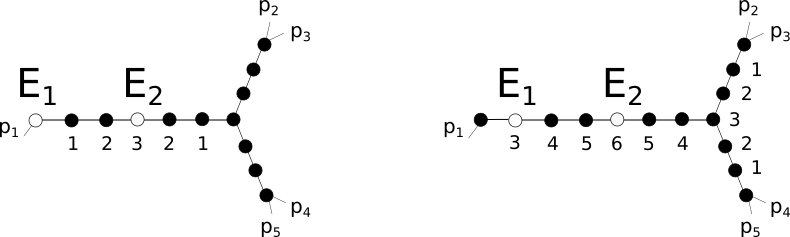
\includegraphics[width=.8\textwidth]{critical_step}
   %\caption{An instance of the critical step, when we pass from contracting the two genus one subcurves separately, to contracting the genus two subcurve as a whole. On the left, the contraction produces a tacnode with a genus one branch, having $\lev_2=3$. On the right, the contraction produces a singularity of type $I_3$. Note that in the meantime we performed a blow-up at $p_1$.}\label{fig:critical}
  %\end{figure}
 We proceed now as in the irreducible case, expanding the circle by $1$ along $T_1$ and by $3$ along all other rational tails.
 \end{itemize}
 
 \begin{figure}[h!bt]
    \centering
    \begin{minipage}[b]{0.45\textwidth}
        \centering
        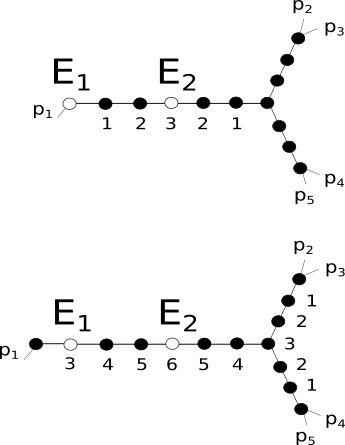
\includegraphics[width=0.7\textwidth]{critical_step_v} % first figure itself
        \caption{An instance of the critical step, from contracting the two genus one subcurves separately, to contracting the genus two subcurve as a whole. Above, the contraction yields a tacnode with a genus one branch, having $\lev_2=3$. Below, the contraction yields a singularity of type $I_3$. Note that we had to blow-up at $p_1$.}\label{fig:critical}
    \end{minipage}\hfill
    \begin{minipage}[b]{0.45\textwidth}
        \centering
        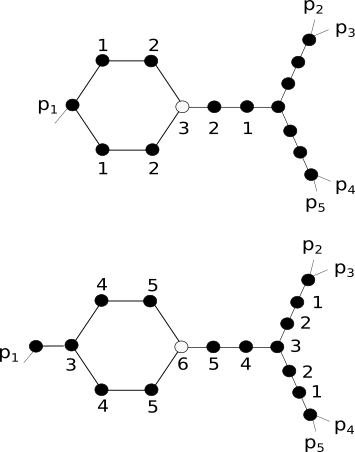
\includegraphics[width=0.7\textwidth]{critical_step_ER_v} % second figure itself
        \caption{Another instance of the critical step, from contracting a genus one subcurve, to contracing a genus two subcurve. Above, the contraction yields an elliptic $3$-fold point with two coinciding branches, having $\lev_2=3$. Below, the contraction yields a singularity of type $I_3$. Note that in the meantime we  have performed a blow-up at $p_1$.}\label{fig:crit_step_ER}
    \end{minipage}
\end{figure}
 
 The case that the central fibre contains two subcurves of genus one, and $p_1$ cleaves to a non-Weierstrass point, is analogous: it is enough to replace the number $3$ by the number $2$, and $2$ by $1$, in the previous argument. The only novelty is, it can happen that $p_1$ is equidistant from $E_1$ and $E_2$, cleaving to the rational chain joining them. In this case we start by expanding a circle around the one with the lowest level; if they have the same level, expand them simultaneously. If at a later stage $p_1$ becomes closer to one of the two circles, we proceed as above, namely by enlarging the circle furthest from $p_1$.
 
 \smallskip
 
 When the core consists of an elliptic curve $E$ with a rational bridge $R$, and $p_1$ cleaves to a Weierstrass point - either on $E$ or on $R$ -, we have noticed above (see the end of Section \ref{rmk:Wandconj}), that $R$ comprises an odd number $k=2h+1$ of rational components. We start as above by enlarging a balanced circle around $E$ in order to establish the level condition \eqref{cond:lev1};  there is a critical step (after which we contract a genus two subcurve, and have to satisfy \eqref{cond:lev2} instead) when the circle touches itself along $R$. This happens after the $(3h+2)$-th step, therefore extending the circle by $1$ along the tail containing $p_1$, and by $3$ on all the other ones, only performs one meaningful step. See Figure \ref{fig:crit_step_ER}. The case of a non-Weierstrass point on the elliptic bridge is analogous.
 
% \begin{figure}
%   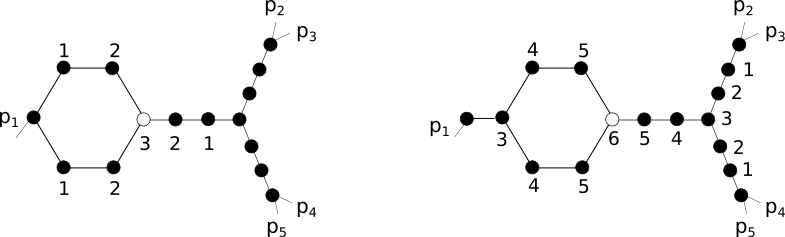
\includegraphics[width=.8\textwidth]{critical_step_ER}
%   \caption{An instance of the critical step, when we pass from contracting a genus one subcurve, to contracting the genus two subcurve as a whole. On the left, the contraction produces an elliptic $3$-fold point with two coinciding branches, having $\lev_2=3$. On the right, the contraction produces a singularity of type $I_3$. Note that in the meantime we performed a blow-up at $p_1$.}\label{fig:crit_step_ER}
%  \end{figure}
  
 \smallskip
 
 Finally, the case that the central fibre has geometric genus zero can be seen as a degeneration of the previous ones, since we only contract a genus zero subcurve when it is a semistable chain.
 \end{proof}
 
 \begin{proof}[Uniqueness of limits] Up to a further base-change, there is a diagram
 \bcd
 & \mathcal C^{ss}\ar[ld,"\phi" above]\ar[dr,"\phi^\prime" above] & \\
 \mathcal C\ar[dr] & & \mathcal C^\prime\ar[dl] \\
 & \dvr &
 \ecd
 extending the isomorphism between the generic fibres, where $\mathcal C^{ss}$ has semistable central fibre and regular total space, by the semistable reduction theorem.
 
 \begin{claim}\label{claim1} If $\mathcal C^\prime_0$ has only singularities of genus $\leq i$ ($i=0,1$), then so does $\mathcal C_0$.\end{claim}
 
 First, assume that $\mathcal C^\prime_0$ has only nodes. If $\mathcal C_0$ has a singular point $x$ of genus one, $E:=\phi^{-1}(x)$ is an \emph{unmarked} subcurve of arithmetic genus one and level $\leq m+1$ of $\mathcal C^{ss}_0$. Then so is $\phi^\prime(E)$: indeed, $\phi^\prime$ being a contraction, it has connected fibres, which bars $\phi^\prime_{|E}$ from being a finite cover of a $\PP^1$. This contradicts the $m$-stability of $\mathcal C^\prime$. We may argue similarly if $x$ is a genus two singularity with $\leq m$ branches. On the other hand, if $x$ is dangling $I\!I_{m+1}$, there is a $-1$-curve $R$ adjacent to $\phi^{-1}(x)$; $\phi^\prime$ must contract $R$ by DM stability of $\mathcal C^\prime$, hence $\phi^\prime(\phi^{-1}(x))$ is again a genus two curve of level $\leq m$.
 
 Assume now that $\mathcal C^\prime_0$ has at worst singularities of genus one, while $\mathcal C_0$ has a singularity $x$ of genus two; the case of a dangling $I\!I_{m+1}$ can be excluded as above. Then $\mathcal C^{ss}_0=Z\cup R_1\cup \ldots\cup R_l$, with $Z=\phi^{-1}(x)$ and $l\leq m$. If $Z$ has geometric genus two, or is irreducible of geometric genus one, $\phi^\prime(Z)$ violates the $m$-stability of $\mathcal C^\prime$. If $Z$ contains a unique subcurve $E$ of genus one, with a rational bridge $R$, then at least one of $R_1,\ldots,R_l$ must be connected to $R$, otherwise $\mathcal C^\prime_0$ - which is obtained by contracting a balanced subcurve around $E$, not including the entire $R$ - would have a positive dimensional automorphism group (scaling a semistable component of $R$). Therefore $\lev(E)\leq (l-1)+2\leq m+1$. Similarly, if $Z$ contains two subcurves of genus one $E_1$ and $E_2$, then $(\lev(E_1)-1)+(\lev(E_2)-1)\leq l$, hence at least one of the two has level $\leq m+1$. In any case, $\phi^\prime(E)$ contradicts the $m$-stability of $\mathcal C^\prime$.
 
 \begin{claim}\label{claim2} We may assume that $\mathcal C^{ss}$ contains either no $-1$-curve, or only one, which is contracted by neither $\phi$ nor $\phi^\prime$.\end{claim}
 
 If there is a $-1$-curve contracted by both, $\phi$ and $\phi^\prime$ factor through a smaller regular model. Assume there is a $-1$-curve not contracted by $\phi$. Then, by condition \eqref{cond:aut}, its image has to be one of the special branches of a genus two singularity; on the other hand, by condition \eqref{cond:p1}, the only special branch of a singularity of type $I$ must contain some special points; therefore we conclude that the singular point $x$ of $\mathcal C_0$ is dangling of type $I\!I_{l+1}$, $l\leq m$. If we let $Z=\phi^{-1}(x)$, we may write $\mathcal C_0=Z\cup R_0\cup\ldots\cup R_l$, with $R_0=R$, and $R_1$ the tail containing $p_1$. 
 By Claim \ref{claim1}, $\phi^\prime$ has to contract a genus two subcurve $Z^\prime$ as well. If $Z^\prime$ is of the shape described in Proposition \ref{prop:contractionII} and it contains $R$, then $Z\subsetneq Z^\prime$ is easily seen, which implies $\mathcal C^\prime_0$ has a singularity of type $I\!I$ with more than $m+1$ branches, by the level condition \eqref{cond:lev2} on $\mathcal C_0$; on the other hand, if $Z^\prime\subsetneq Z$ were disjoint from $R$, then $\mathcal C^\prime_0$ would not satisfy condition \eqref{cond:lev2}. Similarly, if $Z^\prime$ were to be of the shape described in Proposition \ref{prop:contractionI}, then $R_0$ and $R_1$ would have to meet in a ``trunk'' $T$ attached to a Weierstrass point of the core of $\mathcal C_0^{ss}$; if $Z^\prime$ started down along the trunk closer to the core, then $Z^\prime\subsetneq Z$ (so $\mathcal C^\prime_0$ would not satisfy \eqref{cond:lev2}), while if $Z^\prime$ started at the top of the trunk or further away from the core, then $Z\subsetneq Z^\prime$ (so $\mathcal C^\prime_0$ would not satisfy \eqref{cond:sing}). We conclude that, if $\mathcal C_0$ has a dangling $I\!I_{l+1}$ singularity, then so does $\mathcal C^\prime_0$.
 
 \begin{claim} The exceptional loci of $\phi$ and $\phi^\prime$ coincide. \end{claim}
 
 If $\mathcal C_0$ has only nodes, then so does $\mathcal C^\prime_0$ by Claim \ref{claim1}, and we can conclude by the uniqueness part of the stable reduction theorem.
 
 If $\mathcal C_0$ has a genus one singularity $x$, it cannot have a genus two singularity as well, so neither can $\mathcal C^\prime_0$ by Claim \ref{claim1}. If $\mathcal C_0$ has a second genus one singularity $y$, let $E_1=\phi^{-1}(x)$ and $E_2=\phi^{-1}(y)$; they are disjoint balanced subcurves of genus one and level $\leq m+1$ in $\mathcal C^{ss}_0$, therefore $\phi^\prime$ must contract them. Enlarging the contraction radius of any one of them would yield a singularity with at least $m+2$ branches (by condition \eqref{cond:lev1} on $\mathcal C_0$), unless by enlarging we make them touch, in which case we would contract to a genus two singularity; but this is not possible, by Claim \ref{claim1}. The case of a single genus one singularity with a genus one branch, or with a disjoint subcurve of genus one, or with two branches joined by a (possibly empty) rational chain, is similar.
 
 Finally, the case that $\mathcal C_0$ has a genus two singularity, has already been discussed at the end of Claim \ref{claim2}. To summarise, writing $\mathcal C^{ss}_0=Z\cup R_1\cup\ldots\cup R_l$, with $Z=\phi^{-1}(x)$ and $l\leq m$ - the case of a dangling $I\!I_{m+1}$ was dealt with before -, $\phi^\prime(Z)$ must be a point $x^\prime$, by stability considerations. Call $Z^\prime=(\phi^\prime)^{-1}(x^\prime)$ and note that $Z\subseteq Z^\prime$. If $x$ and $x^\prime$ are singularities of the same type, $Z=Z^\prime$ is easily deduced by level/singularity (i.e. outer/inner valence) considerations, the key point being that the shape of the curve has only one parameter (the ``radius'' of the circle), which is determined by $m$-stability. On the other hand, if $x$ were of type $I\!I$ and $x^\prime$ of type $I$, the two special trees determined by $x$ would have to share a trunk attached to a Weierstrass point of the core, and $Z\subseteq Z^\prime$ would imply $Z\subsetneq Z^\prime$, which together with condition \eqref{cond:lev2} for $\mathcal C^\prime$ would make $x^\prime$ into a singularity with too many branches.
 
 The claim follows from observing that the exceptional locus of $\phi$ (resp. $\phi^\prime$) is the union of the fibres $F$ over higher genus singularities of $\mathcal C_0$ (resp. $\mathcal C_0^\prime$), and the rational components with only two special points that are disjoint from $F$.
 
 \begin{claim} The generic isomorphism between $\mathcal C$ and $\mathcal C^\prime$ extends over $\dvr$.\end{claim}
 
 Follows from \cite[Lemma 1.13]{Debarre}.
\end{proof}

Summing up, we have proved the following:
\begin{thm}
 For $1\leq m <n$, $m$-stability defines a proper Deligne-Mumford stack $\oM_{2,n}^{(m)}$ over $\operatorname{Spec}(\mathbb Z[\frac{1}{30}])$, containing $\pazocal M_{2,n}$ as a dense open substack.
\end{thm}
 The restriction on coefficients avoids ramification of the automorphism groups.

\bibliographystyle{alpha}
\bibliography{genus_two} 
 
\begin{comment} 
 
\begin{thebibliography}{AFSvdW17}

\bibitem[AFS16]{AFSGm}
Jarod Alper, Maksym Fedorchuk, and David~Ishii Smyth.
\newblock Singularities with {$\mathbb{G}_m$}-action and the log minimal model
  program for {$\overline{\pazocal{M}}_g$}.
\newblock {\em J. Reine Angew. Math.}, 721:1--41, 2016.

\bibitem[AFS17a]{AFS2}
Jarod Alper, Maksym Fedorchuk, and David~Ishii Smyth.
\newblock Second flip in the {H}assett-{K}eel program: existence of good moduli
  spaces.
\newblock {\em Compos. Math.}, 153(8):1584--1609, 2017.

\bibitem[AFS17b]{AFS3}
Jarod Alper, Maksym Fedorchuk, and David~Ishii Smyth.
\newblock Second flip in the {H}assett-{K}eel program: projectivity.
\newblock {\em Int. Math. Res. Not. IMRN}, (24):7375--7419, 2017.

\bibitem[AFSvdW17]{AFS1}
Jarod Alper, Maksym Fedorchuk, David~Ishii Smyth, and Frederick van~der Wyck.
\newblock Second flip in the {H}assett-{K}eel program: a local description.
\newblock {\em Compos. Math.}, 153(8):1547--1583, 2017.

\bibitem[AK70]{AK}
Allen Altman and Steven Kleiman.
\newblock {\em Introduction to {G}rothendieck duality theory}.
\newblock Lecture Notes in Mathematics, Vol. 146. Springer-Verlag, Berlin-New
  York, 1970.

\bibitem[AK16]{AlperKresch}
Jarod Alper and Andrew Kresch.
\newblock Equivariant versal deformations of semistable curves.
\newblock {\em Michigan Math. J.}, 65(2):227--250, 2016.

\bibitem[Arn72]{Arnold}
Vladimir~Igorevi\v{c} Arnol'd.
\newblock Normal forms of functions near degenerate critical points, the {W}eyl
  groups {$A_{k},D_{k},E_{k}$} and {L}agrangian singularities.
\newblock {\em Funkcional. Anal. i Prilo\v{z}en.}, 6(4):3--25, 1972.

\bibitem[BC20]{BC}
Luca {Battistella} and Francesca {Carocci}.
\newblock {A smooth compactification of the space of genus two curves in projective space (via logarithmic geometry and Gorenstein curves)}.
\newblock {In preparation}, Aug 2020.

\bibitem[BCM18]{BCM}
Luca {Battistella}, Francesca {Carocci}, and Cristina {Manolache}.
\newblock {Reduced invariants from cuspidal maps}.
\newblock {\em arXiv e-print} 1801.07739, Jan 2018.

\bibitem[BLR90]{BLR}
Siegfried Bosch, Werner L\"{u}tkebohmert, and Michel Raynaud.
\newblock {\em N\'{e}ron models}, volume~21 of {\em Ergebnisse der Mathematik
  und ihrer Grenzgebiete (3) [Results in Mathematics and Related Areas (3)]}.
\newblock Springer-Verlag, Berlin, 1990.

\bibitem[Bog99]{Boggi}
Marco Boggi.
\newblock Compactifications of configurations of points on {${\mathbb P}^1$} and
  quadratic transformations of projective space.
\newblock {\em Indag. Math. (N.S.)}, 10(2):191--202, 1999.

\bibitem[BS08]{BalSwi}
Elizabeth Baldwin and David Swinarski.
\newblock A geometric invariant theory construction of moduli spaces of stable
  maps.
\newblock {\em Int. Math. Res. Pap. IMRP}, (1):Art. ID rp. 004, 104, 2008.

\bibitem[Cat82]{Catanese}
Fabrizio Catanese.
\newblock Pluricanonical-{G}orenstein-curves.
\newblock In {\em Enumerative geometry and classical algebraic geometry
  ({N}ice, 1981)}, volume~24 of {\em Progr. Math.}, pages 51--95.
  Birkh\"{a}user Boston, Boston, MA, 1982.

\bibitem[CML13]{C-ML}
Sebastian Casalaina-Martin and Radu Laza.
\newblock Simultaneous semi-stable reduction for curves with {ADE}
  singularities.
\newblock {\em Trans. Amer. Math. Soc.}, 365(5):2271--2295, 2013.

\bibitem[CTV18]{CTV1}
Giulio {Codogni}, Luca {Tasin}, and Filippo {Viviani}.
\newblock {On the first steps of the minimal model program for the moduli space
  of stable pointed curves}.
\newblock {\em arXiv e-print} 1808.00231, Aug 2018.

\bibitem[CTV19]{CTV2}
Giulio {Codogni}, Luca {Tasin}, and Filippo {Viviani}.
\newblock {On some modular contractions of the moduli space of stable pointed
  curves}.
\newblock {\em arXiv e-print} 1904.13212, Apr 2019.

\bibitem[Cuk89]{Cukierman}
Fernando Cukierman.
\newblock Families of {W}eierstrass points.
\newblock {\em Duke Math. J.}, 58(2):317--346, 1989.

\bibitem[Deb01]{Debarre}
Olivier Debarre.
\newblock {\em Higher-dimensional algebraic geometry}.
\newblock Universitext. Springer-Verlag, New York, 2001.

\bibitem[Del85]{Deligne-Gabber}
Pierre Deligne.
\newblock Le lemme de {G}abber.
\newblock {\em Ast\'{e}risque}, (127):131--150, 1985.
\newblock Seminar on arithmetic bundles: the Mordell conjecture (Paris,
  1983/84).

\bibitem[Dem75]{Demazure}
Michel Demazure.
\newblock Classification des germes \`a point critique isol\'{e} et \`a nombres
  de modules 0 ou 1 (d'apr\`es {V}. {I}. {A}rnol'd).
\newblock pages 124--142. Lecture Notes in Math., Vol. 431, 1975.

\bibitem[Dia85]{Diaz}
Steven Diaz.
\newblock Exceptional {W}eierstrass points and the divisor on moduli space that
  they define.
\newblock {\em Mem. Amer. Math. Soc.}, 56(327):iv+69, 1985.

\bibitem[DM69]{DM}
Pierre Deligne and David Mumford.
\newblock The irreducibility of the space of curves of given genus.
\newblock {\em Inst. Hautes \'{E}tudes Sci. Publ. Math.}, (36):75--109, 1969.

\bibitem[Fed14]{Fedorchuk-hyperellipticAD}
Maksym Fedorchuk.
\newblock Moduli spaces of hyperelliptic curves with {A} and {D} singularities.
\newblock {\em Math. Z.}, 276(1-2):299--328, 2014.

\bibitem[FG18]{FedorchukGrimes}
Maksym {Fedorchuk} and Matthew {Grimes}.
\newblock {VGIT presentation of the second flip of $\overline{M}_{2,1}$}.
\newblock {\em arXiv e-print} 1805.08581, May 2018.

\bibitem[FS13]{FS}
Maksym Fedorchuk and David~Ishii Smyth.
\newblock Alternate compactifications of moduli spaces of curves.
\newblock In {\em Handbook of moduli. {V}ol. {I}}, volume~24 of {\em Adv. Lect.
  Math. (ALM)}, pages 331--413. Int. Press, Somerville, MA, 2013.

\bibitem[Gie82]{Gieseker}
David Gieseker.
\newblock {\em Lectures on moduli of curves}, volume~69 of {\em Tata Institute
  of Fundamental Research Lectures on Mathematics and Physics}.
\newblock Published for the Tata Institute of Fundamental Research, Bombay;
  Springer-Verlag, Berlin-New York, 1982.

\bibitem[{Hal}14]{DHLinstability}
Daniel {Halpern-Leistner}.
\newblock {On the structure of instability in moduli theory}.
\newblock {\em arXiv e-print} 1411.0627, Nov 2014.

\bibitem[Has03]{Hassettweighted}
Brendan Hassett.
\newblock Moduli spaces of weighted pointed stable curves.
\newblock {\em Adv. Math.}, 173(2):316--352, 2003.

\bibitem[Has05]{Hassettg2}
Brendan Hassett.
\newblock Classical and minimal models of the moduli space of curves of genus
  two.
\newblock In {\em Geometric methods in algebra and number theory}, volume 235
  of {\em Progr. Math.}, pages 169--192. Birkh\"{a}user Boston, Boston, MA,
  2005.

\bibitem[HH13]{HassettHyeon}
Brendan Hassett and Donghoon Hyeon.
\newblock Log minimal model program for the moduli space of stable curves: the
  first flip.
\newblock {\em Ann. of Math. (2)}, 177(3):911--968, 2013.

\bibitem[HL07]{HL-tricanonical}
Donghoon Hyeon and Yongnam Lee.
\newblock Stability of tri-canonical curves of genus two.
\newblock {\em Math. Ann.}, 337(2):479--488, 2007.

\bibitem[HL14]{HL-birational_contraction}
Donghoon Hyeon and Yongnam Lee.
\newblock A birational contraction of genus 2 tails in the moduli space of
  genus 4 curves {I}.
\newblock {\em Int. Math. Res. Not. IMRN}, (13):3735--3757, 2014.

\bibitem[HLN12]{HLN}
Yi~{Hu}, Jun {Li}, and Jingchen {Niu}.
\newblock {Genus Two Stable Maps, Local Equations and Modular Resolutions}.
\newblock {\em arXiv e-print} 1201.2427, Nov 2018.

\bibitem[HM82]{HarrisMumford}
Joe Harris and David Mumford.
\newblock On the {K}odaira dimension of the moduli space of curves.
\newblock {\em Invent. Math.}, 67(1):23--88, 1982.
\newblock With an appendix by William Fulton.

\bibitem[HM98]{HM}
Joe Harris and Ian Morrison.
\newblock {\em Moduli of curves}, volume 187 of {\em Graduate Texts in
  Mathematics}.
\newblock Springer-Verlag, New York, 1998.

\bibitem[JP18]{PolishchukJohnson}
Drew {Johnson} and Alexander {Polishchuk}.
\newblock {Birational models of $\overline{M}_{2,2}$ arising as moduli of
  curves with nonspecial divisors}.
\newblock {\em arXiv e-print} 1807.09746, Jul 2018.

\bibitem[Kee99]{Keel-bpf}
Se\'{a}n Keel.
\newblock Basepoint freeness for nef and big line bundles in positive
  characteristic.
\newblock {\em Ann. of Math. (2)}, 149(1):253--286, 1999.

\bibitem[KM97]{KM}
Se\'{a}n Keel and Shigefumi Mori.
\newblock Quotients by groupoids.
\newblock {\em Ann. of Math. (2)}, 145(1):193--213, 1997.

\bibitem[Knu83]{Knudsen}
Finn~F. Knudsen.
\newblock The projectivity of the moduli space of stable curves. {II}. {T}he
  stacks {$M_{g,n}$}.
\newblock {\em Math. Scand.}, 52(2):161--199, 1983.

\bibitem[LP17]{Lekili-Polishchuk}
Yankı Lekili and Alexander Polishchuk.
\newblock A modular compactification of $\pazocal{M}_{1,n}$ from
  $\pazocal{A}_{\infty}$ structures.
\newblock {\em J. Reine Angew. Math.}, 2017.

\bibitem[LZ09]{LZ}
Jun Li and Aleksey Zinger.
\newblock On the genus-one {G}romov-{W}itten invariants of complete
  intersections.
\newblock {\em J. Differential Geom.}, 82(3):641--690, 2009.

\bibitem[MFK94]{GIT}
David Mumford, John Fogarty, and Frances Kirwan.
\newblock {\em Geometric invariant theory}, volume~34 of {\em Ergebnisse der
  Mathematik und ihrer Grenzgebiete (2) [Results in Mathematics and Related
  Areas (2)]}.
\newblock Springer-Verlag, Berlin, third edition, 1994.

\bibitem[{Mor}11]{Morrison}
Ian {Morrison}.
\newblock {Mori theory of moduli spaces of stable curves}.
\newblock \url{http://www.projectivepress.com/moduli/moristablecurves.pdf},
  2011.

\bibitem[Pan99]{Pandha}
Rahul Pandharipande.
\newblock Hodge integrals and degenerate contributions.
\newblock {\em Comm. Math. Phys.}, 208(2):489--506, 1999.

\bibitem[{Pol}15]{Polishchuk-nonspecial}
Alexander {Polishchuk}.
\newblock {Moduli of curves with nonspecial divisors and relative moduli of
  $\pazocal A_\infty$-structures}.
\newblock {\em arXiv e-print} 1511.03797, Nov 2015.

\bibitem[RSW17a]{RSPW1}
Dhruv {Ranganathan}, Keli {Santos-Parker}, and Jonathan {Wise}.
\newblock {Moduli of stable maps in genus one and logarithmic geometry I}.
\newblock {\em arXiv e-print} 1708.02359, August 2017 (to appear in Geom. Topol.).

\bibitem[RSW17b]{RSPW2}
Dhruv {Ranganathan}, Keli {Santos-Parker}, and Jonathan {Wise}.
\newblock {Moduli of stable maps in genus one and logarithmic geometry II}.
\newblock {\em Algebra Number Theory} 13(8):1765--1805, 2019. 

\bibitem[Rul01]{Rulla}
William~F. Rulla.
\newblock {\em The birational geometry of $\overline{M}_{2,1}$ and
  $\overline{M}_3$}.
\newblock PhD thesis, University of Texas at Austin, 2001.

\bibitem[Sch91]{Schubert}
David Schubert.
\newblock A new compactification of the moduli space of curves.
\newblock {\em Compositio Math.}, 78(3):297--313, 1991.

\bibitem[Smy11a]{SMY1}
David~Ishii Smyth.
\newblock {Modular compactifications of the space of pointed elliptic curves
  {I}}.
\newblock {\em Compos. Math.}, 147(3):877--913, 2011.

\bibitem[Smy11b]{SMY2}
David~Ishii Smyth.
\newblock {Modular compactifications of the space of pointed elliptic curves
  {II}}.
\newblock {\em Compos. Math.}, 147(6):1843--1884, 2011.

\bibitem[Smy13]{SMY-towards}
David~Ishii Smyth.
\newblock Towards a classification of modular compactifications of
  {$\pazocal{M}_{g,n}$}.
\newblock {\em Invent. Math.}, 192(2):459--503, 2013.

\bibitem[Smy18]{SMY3}
David~Ishii Smyth.
\newblock {Intersections of psi-classes on moduli spaces of m-stable curves}.
\newblock {\em arXiv e-print} 1808.03214, Aug 2018.

\bibitem[{Sta}19]{stacks-project}
The {Stacks Project Authors}.
\newblock \textit{Stacks Project}.
\newblock \url{https://stacks.math.columbia.edu}, 2019.

\bibitem[Ste96]{Stev}
Jan Stevens.
\newblock On the classification of reducible curve singularities.
\newblock In {\em Algebraic geometry and singularities ({L}a {R}\'{a}bida,
  1991)}, volume 134 of {\em Progr. Math.}, pages 383--407. Birkh\"{a}user,
  Basel, 1996.

\bibitem[vdW10]{vdW}
Frederick van~der Wyck.
\newblock {\em Moduli of singular curves and crimping}.
\newblock PhD thesis, Harvard University, 2010.

\bibitem[Vis12]{VISC}
Michael Viscardi.
\newblock {Alternate compactifications of the moduli space of genus one maps}.
\newblock {\em Manuscripta Math.}, 139(1-2):201--236, 2012.

\bibitem[VZ08]{VZ}
Ravi Vakil and Aleksey Zinger.
\newblock {A desingularization of the main component of the moduli space of
  genus-one stable maps into {$\mathbb P^n$}}.
\newblock {\em Geom. Topol.}, 12(1):1--95, 2008.

\bibitem[Zin09]{Zingerred}
Aleksey Zinger.
\newblock Reduced genus-one {G}romov-{W}itten invariants.
\newblock {\em J. Differential Geom.}, 83(2):407--460, 2009.

\end{thebibliography}

\end{comment}

\end{document}
